%%%%%%%%%%%%%%%%%%%%%%%%%%%%%%%%%%%%%%%%%
% The Legrand Orange Book
% LaTeX Template
% Version 3.1 (February 18, 2022)
%
% This template originates from:
% https://www.LaTeXTemplates.com
%
% Authors:
% Vel (vel@latextemplates.com)
% Mathias Legrand (legrand.mathias@gmail.com)
%
% License:
% CC BY-NC-SA 4.0 (https://creativecommons.org/licenses/by-nc-sa/4.0/)
%
% Compiling this template:
% This template uses biber for its bibliography and makeindex for its index.
% When you first open the template, compile it from the command line with the 
% commands below to make sure your LaTeX distribution is configured correctly:
%
% 1) pdflatex main
% 2) makeindex main.idx -s indexstyle.ist
% 3) biber main
% 4) pdflatex main x 2
%
% After this, when you wish to update the bibliography/index use the appropriate
% command above and make sure to compile with pdflatex several times 
% afterwards to propagate your changes to the document.
%
%%%%%%%%%%%%%%%%%%%%%%%%%%%%%%%%%%%%%%%%%

%----------------------------------------------------------------------------------------
%	PACKAGES AND OTHER DOCUMENT CONFIGURATIONS
%----------------------------------------------------------------------------------------
\documentclass[
11pt, % Default font size, select one of 10pt, 11pt or 12pt
fleqn, % Left align equations
a4paper, % Paper size, use either 'a4paper' for A4 size or 'letterpaper' for US letter size
%oneside, % Uncomment for oneside mode, this doesn't start new chapters and parts on odd pages (adding an empty page if required), this mode is more suitable if the book is to be read on a screen instead of printed
]{LegrandOrangeBook}

% Book information for PDF metadata, remove/comment this block if not required 
\hypersetup{
	pdftitle={Title}, % Title field
	pdfauthor={Author}, % Author field
	pdfsubject={Subject}, % Subject field
	pdfkeywords={Keyword1, Keyword2, ...}, % Keywords
	pdfcreator={LaTeX}, % Content creator field
}

\addbibresource{sample.bib} % Bibliography file

\definecolor{ocre}{RGB}{243, 102, 25} % Define the color used for highlighting throughout the book

\chapterimage{Images/orange1.jpg} % Chapter heading image
\chapterspaceabove{6.5cm} % Default whitespace from the top of the page to the chapter title on chapter pages
\chapterspacebelow{6.75cm} % Default amount of vertical whitespace from the top margin to the start of the text on chapter pages

%----------------------------------------------------------------------------------------

\begin{document}
	
	%----------------------------------------------------------------------------------------
	%	TITLE PAGE
	%----------------------------------------------------------------------------------------
	
	\titlepage % Output the title page
	{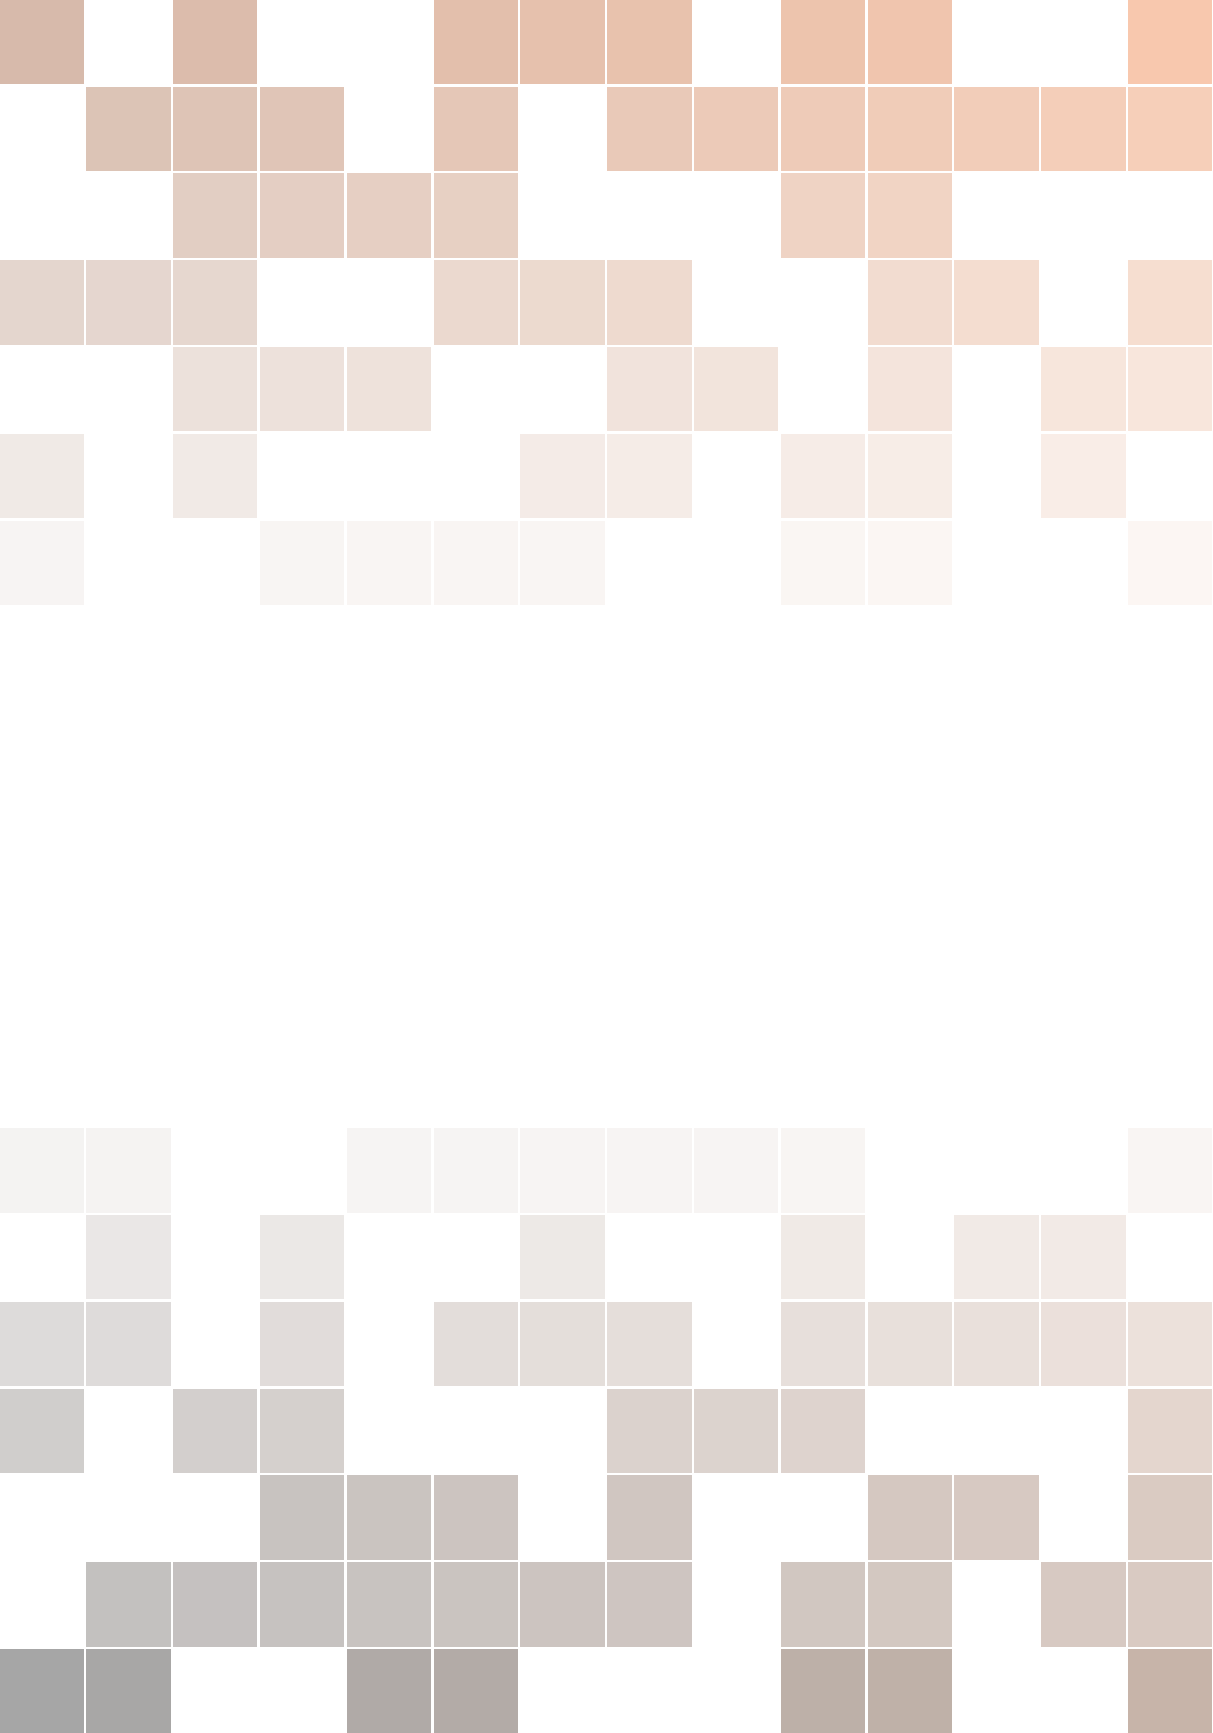
\includegraphics[width=\paperwidth]{Images/background.pdf}} % Code to output the background image, which should be the same dimensions as the paper to fill the page entirely; leave empty for no background image
	{ % Title(s) and author(s)
		\centering\sffamily % Font styling
		{\Huge\bfseries Micro and Nano Systems Track\par} % Book title
		\vspace{16pt} % Vertical whitespace
		{\LARGE A Micro Journey in a Nano World\par} % Subtitle
		\vspace{24pt} % Vertical whitespace
		{\Huge\bfseries Lorenzo Vergata\par} % Author name
		%\vspace{6pt} % Vertical whitespace
		%{\bfseries Whisper Large V3\par} % Author name
	}
	
	%----------------------------------------------------------------------------------------
	%	COPYRIGHT PAGE
	%----------------------------------------------------------------------------------------
	
	%\thispagestyle{empty} % Suppress headers and footers on this page
	
	%~\vfill % Push the text down to the bottom of the page
	
	%\noindent Copyright \copyright\ 2024 Lorenzo Vergata\\ % Copyright notice
	
	%\noindent \textsc{Published by John Doe}\\ % Publisher
	
	%\noindent \textsc{\href{https://www.latextemplates.com/template/legrand-orange-book}{book-website.com}}\\ % URL
	
	%\noindent Licensed under the Creative Commons Attribution-NonCommercial 4.0 License (the ``License''). You may not use this file except in compliance with the License. You may obtain a copy of the License at \url{https://creativecommons.org/licenses/by-nc-sa/4.0}. Unless required by applicable law or agreed to in writing, software distributed under the License is distributed on an \textsc{``as is'' basis, without warranties or conditions of any kind}, either express or implied. See the License for the specific language governing permissions and limitations under the License.\\ % License information, replace this with your own license (if any)
	
	%\noindent \textit{First printing, \today} % Printing/edition date
	
	%----------------------------------------------------------------------------------------
	%	TABLE OF CONTENTS
	%----------------------------------------------------------------------------------------
	
	\pagestyle{empty} % Disable headers and footers for the following pages
	
	\tableofcontents % Output the table of contents
	
	%\listoffigures % Output the list of figures, comment or remove this command if not required
	
	%\listoftables % Output the list of tables, comment or remove this command if not required
	
	\pagestyle{fancy} % Enable default headers and footers again
	
	%\cleardoublepage % Start the following content on a new page
	
	%----------------------------------------------------------------------------------------
	%	PART
	%----------------------------------------------------------------------------------------
	
	\part{Nanoelectronics of Graphene and Related 2D Materials}
	
	\chapter{Magnetostatics}
The course is trying to bridge the gap between a fundamental aspect of magnetism and the real application of magnetism in real life. And I was just making this example that's been between you as a student from my group who is really working to the redesign of the magnetic field sensors. But for doing this he needs all, I'll say, all the ingredients that I tried to explain during this course. That's the reason why he's attending the course because it's not coming from physics engineering. So this course was missing in his career. A friend of mine, who's not just a friend, he was the past president of the European Magnetic Association, the name is Burka Hillebrand, who is the father of Magnolian Westerners, who is used to say that Ricardo, you have a double soul. You are a physicist but also an engineer. Obviously it's true, my degree is in electronic engineering, but in the end my PhD is in physics and I'm giving a lecture in physics. But okay, what I try in my life is really to establish sort of a bridge between academia and companies and so on, because this is our real life at the end of the day. Mathematics is very beautiful, but what is the day-by-day implication of that? Now I will try during this course to make some example which really can be used to bridge the gap to show how quantum mechanics begins real application also in the field of back end of production.\\
Basic magnetostatics, which is now the topic of today's lecture. Understanding what happens in statics. Magnetostatics means state-stage system. We are not talking about in waves, permanent regression dynamics, static configuration of a magnetic bond. which means not just iron and an infinite crystal, but a piece of iron. It is shaped as a sphere, the film, the bar, the shape makes the difference. And magnetostatics deals with the static configuration of the magnetization, not the field created by the magnetization. In some sense, this is the physics of three magnets. Okay, when you have a three magnets, you can play with magnets. And you know, if you know this game, which is your mind. You're playing with German. Yeah, that's a good starting point for this. Get to play. So you understand the magnetic force magnetism. And what's your name? I sound good. That's the names of today. It's been so let's start with when you play with the German. I give Pearson is the right-hand pole, he is the left-hand pole, North, North, and South Pole. So we have to understand the physics of the geometry. Okay. First of all, let's review which are the main characters of this course and the basic equation that you have.
\fig{2}{lecture_1 basic magnetostatics.pdf}
So you have different characters and things. B, H, and L. Okay. Well, the three guys are feeling this one. B is the induction field. H is the magnetic field. M is the magnetic solution. Let me just review the meaning of this. Which is the difference? Sorry. I apologize. I apologize. M is the magnetization. What's the definition? It's the magnetic moment that you are holding. Magnetic moment that you are holding. So what does it mean? How do you measure a magnetic moment? Magnetic moment, you should always refer to the idea of the circuit, so the magnetic moment is measured in water. It's the intensity of the current multiplied by the area. And when we go to the magnetization, we need to realize that magnetization is measured in water. Current by surface divided by volume, to the current divided by a light. That's why in terms of units, it is measured in amps per meter. That's the unit of the magnetization of the International System of the Universe, in which we will live and be. I made this choice in the very beginning, not purely for the different systems that I'm using in physics. I'm using now the International System of the Universe. amps per meter. And then you have the induction field B and H. I ask you, what is the difference between B and H? I do not completely agree. the example for HF. Okay, the relation is this one. B is equal to 0H plus F. Okay, that's the definition. But physically, you have to say what is the difference between B and H. But for that, B is the vector appearing in the Lorentz field. So an electric charge is moving in a magnetic field with the Lorentz force, 2B cross B. and is B the field which determines now the force acting on the magnetic field? It is B. H is something slightly different because H is connected to what? The current. The connection is quite straightforward. You know that the curl of H is equal to J Not only this, but what should I have here? Maxwell equation, one hundred most beautiful things of every size, plus, plus root. Something is missing. Yeah. You can write in the free space or otherwise you can write in the derivative of D, with respect to the time. But for today, if you write in magnetostatics, you can also forget about this one. Magnetostatics means the states of the oscillation of the coordinates of the light and the field is not changing. But you immediately see that H is directly connected to the source of the magnetic field, which is usually connected to the current flowing in a wire. But this is not the unique vision of the story, especially magnetostatics, also because when the free space but their current amount, no. Obviously, the field is going to be better. And what is now the problem or the opportunity? The opportunity is here, B, as you see, the museum, EH plus M, okay? So, and the H can be reduced by the magnetization itself. So, what is the Fritz magnet? The Fritz magnet is made of an odd magnet, typically a cobalt, a boron, or a chloride, which displays a nice, realistic look. So, at zero, external field, you have a net Riemann magnetization. And so, this is the source of the H, okay, especially magnetostatics. In magnetostatics, when you say What does it mean? There are no currents of one in the center. That's the framework in which we are more. So the the derivative we expect to time are equal to zero and no current. So the sources of the magnetic field are not connected to cards, but connected to the presence of the body which is magnetized in remnants due to the fact that it's a full magnet due to exchange interaction with a remnant magnetization at zero external field. And that's the reason why when you move from there to this relation here, you usually find that B is equal to mu zero, HM plus M. And this subscript M is here just to tell you that this is the H field not produced by the current here. The J zero here, okay, is produced by the magnetization itself, okay? So no current means that the H is not produced by J. So this means also that the curl of H equal to zero. Okay? This is zero. And that's the reason why in magnetic structure, at values with the general framework of electromagnetic you can define what is gamma retention. The reason is quite heavy, it is immediately evident. If you see that you have a vector h whose curl is equal to zero, but this means that you can write h as the gradient of something else, a kind of field, exactly as in order as in order to start. So you can say that, okay, so if this is the story, I can write immediately H is equal to minus the gradient of a scalar potential U. Usually you cannot do that. So the kernel of H is equal to U, not because we are trying to use the vector equation. But this is not the case. Here you can use a standard equation. And there is another story which is also relevant here. In terms of units. I didn't feel completely stable here. M is the magnetization which must be expressed in m per meter. But according to this equation here, here, m and h, they have the same units, okay? This is quite evident. So h, again, in amps per meter, so if you want this magnetic field, and this is the induction field. and the magnetic field must be measured in m per meter and as you have this pointed here this constant which is near zero which is the back of the mobility 4, 5, 8, 10, 11, 17 units in the initial system it does all that it also has it's not dimensionless this one So then the unit for B is Tesla, okay? In the international system of units. B is measured in Tesla, M in the international system of units. Okay, so these are the three characters of magnetostatics. The basic equations are these two equations here, and from these you immediately realize that you can use the scalar potential, which is much easier for multiplication. Scalar potential. And now, what's the impact of this? Immediately you realize that you can apply the same mathematics over the rhythm of statics. So we have the scalar potential, h is minus the gradient of u, which is like the case of e, given to e, but minus the gradient of p. And so, okay, and so. And so what happens? You can say okay, but if you have this equation here, you immediately find that you can write down a Poisson or Laplace equation for the magnetic star hypotension. And how it goes out? So it's very simple. So do not forget that B is always true that the divergence of B is equal to zero. Because there are no magnetic monopoles. The divergence of B is always C. So essentially, you have it, okay? The divergence of B is equal to zero, but B is mu zero by H plus M. This means that the divergence of H is equal to minus the divergence of M. Okay? And then instead of H, you can replace minus the gradient of U, and this means minus the number of squares of U, which is equal to minus the divergence of M, and so your your language with this equation. The Poisson equation, okay? The Poisson equation is the number of squares of Q which is equal to the divergence of M. It's very similar to something that you know. Number of squares of B is equal to minus O divided by epsilon Z. Okay, it's again a Poisson equation. And so from the analogy that I started to tell you about, this seems to be related to sort of charge. And indeed we will see that it's exactly connected to the concept of magnetic charges. But okay, let's continue this discussion. So we are here, we have this equation here, It's a sort of Poisson equation. Inside the magnetic body, you have a diagonal. You have an M, okay? Don't forget that in general you have a magnetic body with a volume, surface, and the norm under the surface, N, according to this. And inside the body, you have a non-moon diagonalization, so you can have a 30-D-L. It can be zero or not, depending on the divergence of M. But you can have it. But outside the magnetic body, there is no M, M is zero, the divergence of U is zero, then you have not a Poisson equation, but a Laplace equation. now the square of u outside must be equal to zero. And now you have this Laplace equation plus some equation. That's a typical problem that we have seen in electrostatics, and so one can say it's the answer. Of course, we have some boundary conditions, because we have an equation inside, an equation outside, now without the boundary conditions. We will see afterwards that the boundary conditions for U at the surface are these two conditions. The continuity of the U is very similar to the continuity of the electric field. The electric field can admit this continuity, not the tension, otherwise there is a divergence. And there is another condition, which is this one, stating that if you calculate now the derivative, the direction of the derivative, the derivative of u with respect to the direction to the norm of the derivative inside, you subtract the same direction of the derivative outside, immediately inside, immediately outside, this is equal to m dot. We will see that this is exactly the same condition that you are used to, stating that the normal component of B must be conserved when you cross a little bit between the two points. But okay, you have this regulation, and you have this binary condition, and provided that you find a solution which is regular at infinity, which corresponds to this condition here, condition, a fantastic condition, a fantastic situation, so that if by inspection you find a solution, that the solution is not a second solution. This genus theory is an extremely powerful tool for solving magnetic static. And this is a very powerful method for solving the problem that we will see.
\fig{3}{lecture_1 basic magnetostatics.pdf}
Now, as I was telling you, this is a negative sign. That could be also an exact sign. That's exactly this one. So, demonstrate that the boundary condition that you are used to from general courses of the electromagnetic state in that when you cross an interface, the parallel component of H and the perpendicular component of B, not B, show that these are equivalent to the following conditions, exactly the conditions I told you about. So let's solve this exercise, just to work it out. So one could start with the condition for the conservation of perpendicular components of B. So what happens? Let's imagine that you have neutral states between two magnetic materials, different magnitudes. This is inside, so let's imagine that, okay, this is your body, okay, so you are here, and here it's outside, okay. So the typical story that you know is that inside and outside the perpendicular component of B must be equal. So B in perpendicular must be equal to B out, okay? This is B. But now what about B? B is mu zero by m plus h. Inside you have m, outside you don't have m. So this is your body, outside you have a vacuum, but it's no magnetic material. So inside you have to write down mu zero m plus h m. Okay, inside. So, outside you have what? Mu zero, h m, no longer there. So mu zero, you don't need it. And now you have what? Okay, m. But you have to take what? The perpendicular component. So this gives y. So you take the projection on the normal, the unit vector which is normal to the surface, which is n. So let's assume that here you have this n. So you take m dot m plus volt. Okay, let me say that this hm can be written like minus, what is it? H is minus the gradient of u inside. So you have minus the gradient of u in dot m, u in dot n, which is equal to h outside, same story, minus the gradient of u out dot n. But when you take now the scalar product between the gradient and the normal, what are you find? r is the direction of derivative along the direction of the norm. You project the gradient in the direction to find the partial derivative along that direction, to the So, in the end, you have m dot n. So what is this? Minus partial derivative of u in with respect to n, equal to minus partial derivative of u out with respect to n. And this is exactly the condition which is reported there. So in the end you find out that the discontinuity and the partial derivative from inside and outside is equal to m dot n. Okay? Good. First condition, which is demonstrated, so the equivalence is demonstrated. you have a cycle one just that concerning the fact that the parallel component h in parallel might be concerned but be equal to h out of that and here i say what you say it is automatically satisfied i told you that h is equal to minus the gradient of U but okay this means that the curl of H is 0 okay no way curl of H is equal to 0 if the curl of something is equal to 0 it's very easy to demonstrate that you take a path like this and you integrate the curl this means the circulation over this line must be zero, and this automatically brings you to the conclusion that the true pilot component must be equal. Automatically . And then, what's the origin for the continuity of the U inside and outside? It's not connected to a very simple show. As H is equal to minus the gradient of U, It's evident that if you have a discontinuity in the U, you will have a divergence in H. And you want to avoid this divergence, which is unphysical. It's exactly like an electrostatic. In electrostatics, you can have a discontinuity in the electric field, but not discontinuity in the potential. So if you are discontinuating the electric potential, there is a divergence of the electric field at that boundary. here is exactly the same thing. So when you write down these conditions, you ensure that H is according to which is well defined without divergence, and you are ensuring that the parallel component of H is conserved and what's the curtain in your component is conserved. Okay, so this is an exercise that I'm used to to solve. Are you okay? What's the name? You also fear that you won't qualify. Sorry, just trying to recognize the face. So, it's an exercise just to make some practice with Maxwell equations, which could be also nice for restarting a little bit at the beginning of this course. OK, but now what's the point? We found that we have an equation which is nice, which is an equation in which you are essentially look at this part here.
\fig{4}{lecture_1 basic magnetostatics.pdf}
It's a Poisson equation. This slide is meant to establish a full analogy between magnetostatics and electrostatics. Look, for the magnetic material, we have that B is equal to 0H plus M. For a dielectric, we have that D is equal to epsilon zero by E plus P. What is P? is the polarization effect is measured in two more room meters squared. And so you see that there are three characters with some correspondence. So B, the meaning of D, the electric field H, and instead of M, you have B. And those are physically you understand that the meaning is very similar the polarization that you can have in the material has the same function the functionality of the magnetic solution and as a matter of fact the equation described in ferroelectrics and true magnets are very similar the long dowel potential for both systems is exactly the same so the same properties can be you have a coercive field, an inferred magnetism, an electric field, you have saturation, remnants, you have a coercive field and also a loop, an integrated loop, anyway. Now, H is equal to minus, gradient of U, but E, the derivative is minus the gradient of H. One to one. There is a difference. The divergence of B is zero. That's a big difference. the divergence of E, the Gauss theorem, is equal to the density of charge divided by the density of E. But in terms now of the equation that you find, here you have the number square of U, which is equal to the divergence of M, and in that case, you have the number square of B is equal to minus 4 divided by absolute E. So, let's use now the thermo-centrifugal climate. The same equation has the same solution. How can you apply this central theory? Because, okay, what are you used to apply in eletrosclerosis to solve the problem? You say, okay, I have this equation. Now, forget about the left problem. Now, the density of charge that we put there is the sum of two contributions. We can have three charges, those appearing at the surface of the components, and polarization charges, those appearing in dielectrics, either at the surface or even in the volume, depending now on the condition of polarization of the volume. But what is the solution for the problem of the electrostatic? We can write down the expression for the potential, starting from the superposition principle and the solution for one charge. So that you can say that as the source for the electric field are water, the potential, the free charges on the conductor and the polarization charges, we can write down this equation saying that okay the road to be placed here is the sum of three row three density of charge minus the divergence of the example is the way you write down the density of polarization okay so let's assume that row three is see what you see. I'm not coming back to it. So I just left with a dielectric material which is polar. It's exactly what you have on this side for the main of the star. You don't have electric current here. The equivalence story is we don't have electric charges to the mass. So, the Poisson equation becomes the number squared of V is equal to minus by minus the state of space plus the divergence of space divided by epsilon. This is the equation, and the solution is something that you know very well. The solution is this one. V is equal to one divided by four pi f multiplied by one, the sum of two into one. The first one is the contribution to the electrostatic potential coming from the volume of the charge. C minus the divergence of P in the R-th parameter, divided by R minus R-th, contribution from the volume charges of polarization, plus the contribution from the surface charges of polarization, P dot n. Okay, this is the really the surface density of collision charges divided by r minus r prime integrated over x. This is the solution of the equation. But now you can say, okay, the density, the volume density of collision charges is minus the derivatives of p and the surface density of collision charges is p. Now you go back and say, okay, but here I have this equation and the other equation. So now you can say, okay, same equation, same solution. Strong parallelism, you say, okay, let me write down instead of v, u. Here you have 1 divided by 4 pi epsilon zero. Okay, here you have epsilon zero, here you don't have something at the denominator. So just 1 divided by 4 pi, multiplied by the sum of two integrals. The first integral would be a volume integral, same here. divergence of P, but P, in this case, is m, so minus the divergence of m, divided by r minus r prime, integrated over the surface. Then you move to the integral over the surface, that was here P dot m, what do you find here? m dot m, divided by r minus r prime, integrated over the surface. And that's the solution for U. You see the strong analogy between the two things, same equation, same solution. So you have found now the connection between the magnetization and the U. And the problem is solved once forever, because now if you know the distribution of M, you You can calculate the U and if you can calculate the U, H is equal to minus the gradient of U. End of story. You see my point? The problem is solved. And now there's another column. Do you have a question? Yeah. I'm not sure. Yeah. It's another idea. Right. Is the analogy so that when we are talking of charges in the dielectric field, the corresponding is the charges and the corresponding is current. Exactly. So, by analogy, volume and energy charges are current in this case. Are you referring to this slide? Yeah. So you're asking me something before I explain that. Just go. What is that? I have something. I have something. I have a signal. I have something. Okay, one neuron remains. It's a big issue. Sorry. Okay. Let me first make a comment and then probably the solution, the question, the answer to to your question should be quite clear. Let's now make a comparison between this solution for U and that solution for V. You immediately try to associate this minus divergence of M with the minus divergence of P. But as minus divergence of P is the density of polarization charges, You introduce this concept, which is a pure mathematical concept of volume magnetic charges. As you see, minus the radius of P is physically a volume density of the partition charges. Okay, so this term, BA, is like a volume density of something that I call by analogy magnetic charges. Do magnetic charges exist? No. It's just a pure mathematical concept that you are using in order to explore the analogy. Okay? They do not exist. So the divergence of B is equal to zero. Okay? only the Naomi dipole exists so far, okay? Who will demonstrate something else with the normal price, millions of dollars, for the time being, is pretty much equal to zero. So this means that it is just a mathematical term that is useful and can be helpful when you try to solve a problem, but it's a mathematical term and by analogy. What about m dot n? p dot n is a surface polarization charge density. So you say that m dot n is like a surface magnetic charge density. Okay? Why it's so relevant to your theory? not everybody loves this kind of approach. People say, okay, now you have to use the vector potential in a way, why are you running with the scalar potential? But in practice, you will see in a while that establishing a sort of parallelism, like the static problem, ending with a static one, is very powerful because it because it provides you with an immediate vision of what is going on in the magnetic field, starting from the concept of the electrostatic process. You know very well, you are not used to work with magnets, you are more used to work with electric charges, potential and so on, so you can now use what you know from the electrostatic and apply it to you. That's more or less the A very simple example would be this one, and then we will take a break, otherwise the lecture will become too long. So you know what's the origin of magnetism, of the name magnetism? You know the origin. You know magnetite. Magnetite there, okay, what is magnetite? It's a rock, okay. So magnetites come from magnetite, okay, but which is not the end of the story. to magnetize In iron free Is a rock but who gave the name magnetized to this rock With bricks they did they gave the name to her to everything They just they discovered everything and also the final that we were just making something final everything was done by greeks So yeah, the Greeks, which Greeks living in which city? Is he famous? Was he a philosopher? Okay, but he's connected to Magnetism. It's Magnesia, the city of Magnesia. Magnetism comes from the city of Magnesia, Magnetism comes from the city of Magnesia, in Italy, the station of Magnesia. And that magnetism came. They discovered the property of this rock around the 7th century B.C. And they were typically playing with this rock shaped in the form of a bar. Like in the German. For a reason that I will explain in a while, when you have a bar or a through-magnetic body, it displays a natural tendency to develop the remnant magnetization along its axis, Which means that you can imagine that M is uniform and is directed along the axis. But now let's imagine that you have a cylinder which is uniformly magnetic. Quite low. Do you have some magnetic charges inside or at the surface? Let's imagine that it is uniform. there are no volume magnetic charges, so the divergence of M is 0. No magnetic charges inside. Are there some surface magnetic charges? So you have to calculate M dot N. And now you have two possibilities. This is N here, but M dot N is 0. zero, you don't have magnetic charges on the surface, on the lateral surface of the cylinder. Nothing. Zero. But what happens here? Here you have N1 and here you have N2. And you discover that M dot N1 is positive and on the other side you have sigma 2 which is m dot n2 which is negative. So you can now say that mathematically you can think about some positive magnetic charges here, some negative can be charged there. And now let's imagine that you have a problem like this in a leg of a car. Which kind of field do you expect to see? You know the solution. The field lines are expected to be like this. Which is exactly the solution for the magnetic field produced by a valve end. That's the reason why he played with the German. Because if you have a cylinder which is uniformly magnetized along the direction of heat, Hartz's, you just have some magnetic charges concentrated at the two extreme portions, at these two phases. So these are the the north and south poles interacting differently, okay? Positive and negative charges. Two positive poles, they repel each other. Two poles with opposite sides. But, I think it's exactly this. And this is just a pretty simple example explaining why disposable magnetic charges can be very, very helpful. We will review his many, many facts, but from now on, we will leave it. quantitative and elegant way.
\fig{5}{lecture_1 basic magnetostatics.pdf}
So essentially we have the problem of an infinite cylinder with an axis along z in this x, y, z reference frame. And let's assume that the infinite is physically, unphysical, but it's a mathematical simple problem describing a long cylinder. It is the same that I just tried to solve here, in which we are putting the charges far and far away. Now M is uniform in size. It means you take the magnetic material, you shape it into a cylinder, you magnetize it in the Z-direction and okay, the problem is there. Which is now the magnetic field. The B is H, produced by this distribution of magneticization. So we know that the equation is always the same with the Poisson equation, but in this case, as M is uniform inside, We can't argue that there are no quantum magnetic charges, that the Poisson equation becomes a class equation. The number of squares of u is equal to zero. And the general equation of this is what? The number of squares of u is equal to the divergence of m. But as m is moving from the inside, the radius of m is 0, and we are left with a log-Nagel situation. Clearly, in this case, it is useful to work in cylindrical coordinates. The double-square assumes this form. When you are using rho, which is the radial coordinate, phi, which is dv, the azimuthal hangar here in the x-1 plane, and z, of course, which is the coordinate of the axis of the plane. So this is the representation of the Laplace equation, and what about the boundary conditions? Boundary conditions here are connected to the possible presence of modes of magnetic charges. But in this case, you don't have magnetic charges. reason is quite simple, because m dot n is equal to zero, m dot n, they are perpendicular. So there are no magnetic charges on the lateral line of the solution, okay? No charges there, and in this case, there are no magnetic charges at the top and at the bottom, because at the top and the bottom, they do not exist. They are an infinite cylinder, or they are put at infinite So boundary condition becomes this one. So there is a continuity in the partial derivative with respect to the n, which is the body of the constant. And you know that you must have a complete condition. How do you solve this equation? Don't forget that if the solution exists, it's unique. What is the trivial solution of that equation? Respecting the boundary. U equals the constant. Okay? Because if U is equal to the constant, perfect in the sense that, okay, the equation here is partial derivative equation, equation, the automatic density is zero. And, of course, the two partial derivatives equal to zero, and there will be a continuity of the U from inside to outside. So, immediately you find that this simple solution that you see by height, by inspection, is U equal to zero. Okay? And now what is the implication of u equals to zero? What are you looking for? You're looking for h. h is minus the gradient of u, which is equal to zero. So what's the implication? h is equal to zero everywhere. Okay? Everywhere. Does it make any sense to you? You have a material which is uniform and magnetized and if it is linear and H is equal to zero Is it possible that it makes sense? Or some Is Can you find any connection between this problem and that problem? This one. This problem transforms into that problem if you do what? If you put these two faces at minus infinity and plus infinity. But what's the impact? We have magnetic charges at infinite distances that do not create a magnetic field where we are. You see? But in case of the 11th time, if you have some elliptic charge that place at plus infinity and noise infinity, it will not produce a 5, it will be a ui. You see the point? So it makes sense. Here, it makes sense. So you have that H is 0 everywhere. What about B? Is it 0, B? No. So, B. So, H is equal to zero, but B is equal to mu zero H plus M. So, you have B is equal to mu zero M. So inside the cylinder, you have m and you have b, and they are parallel. b is equal to mu0, but we don't have h. So h is equal to 0, and h must respect the statement as the surface, there must be a continuity in the parallel to the point of h. If h is 0 inside, it's also 0 outside. But let's go back to the other. This is for an infinite cylinder. And in that case, in the previous one, this was H out. What about H inside? In the case of a finite cylinder, H inside. could be now the orientation, the direction of age inside? What's your name? Sorry. Eduardo. Eduardo. What do you mean? From right to left or from left to right? But so it all this proposed in like this age in Do you agree What's your name Why do you say the opposite you have to H parallel inside and outside, they must be equal. So it's impossible to add this. You see my point? That's impossible. Because this will violate the conservation of the tangent of the parallel component of H. So, H inside would be like this. And this is totally coherent with the analogy with electrostatics. Because in electrostatics, the electricity goes from positive charges to negative charges. And in magnetostatics, it's exactly the same. The magnetic field H goes from positive charges to negative charges, both inside and outside. So this is the unique possibility that you have. Pay attention to one fact. H inside here opposes the magnetization. That's the reason why it's called demagnetizing field. the fact that you create a surface, it creates some, so you're creating some magnetic charges at surface, and they generate a field which opposes the magnetization. It's a demagnetizing field, which tends to demagnetize your body. Okay? Okay. So coming back here, that's the reason why you say H in is also called H demagnetizing or HM or H in. Demagnetizing field, magnetostatic field produced by the magnetization or H inside. Just different names. But this is a very fundamental concept. So there is a demagnetizing field, which opposes the magnetization, due to the fact that you have some surfaces. You have a finite volume to be applied by the magnetization. In case of the infinite cylinder, there are no magnetic charges, so, the charges are plus infinity, minus infinity, they are not able to create a demagnetizing field here that's equal to Z. So then B is equal to mu zero by N. So in this sense, the maximum B that you can have is that for an infinite cylinder. Because you are during the demagnetizing field. Okay? And then, okay, there is a strange story here that we have to review in a while. Let's see, so EM, what is EM? EM stands for magnetostatic energy. Something that can be seen is that the magnetostatic energy in this case is equal to zero. I will try to review this concept afterwards, after explaining in more detail what is magnetostatic energy.
\fig{6}{lecture_1 basic magnetostatics.pdf}
Let's solve another problem. Just very, sorry. Yeah, this one is very similar to the previous one Jogging is exactly the same In your infinite cylinder that you're ready to are but now it's my it is magnetized along X direction to the right of it Big magnet and the other song and the top three it can be my reward the magnetizing on the x-axis. But now what's the field produced? Are these perfect or not? The question is completely, but now you expect to see some magnetic charges on the moon. Now same machinery and you say okay So this is the first case second case here Nothing changes here. Okay again M is uniform inside which means that the equation is always the same Yeah, then Navla squared of U is equal to 0 now the boundary condition So the equation is always the same but the boundary condition are different The boundary condition is the boundary condition are expressed like this So Let's me do something This X is Y and then this point towards you. Okay, so this is a cross-section In your circle radius are So it's not very good The magnetization is Pointing please This is m. Okay. And now, let's write down the boundary condition. Boundary condition is saying that the derivative of u in psi with respect to r does it... Let me say that, for instance, I'm taking this angle, which is the angle phi, the n as a normal, like this. Okay? And so when I take the partial derivative with respect to n, I'm taking the partial derivative with respect to the value of the insulated asymmetry. So it is the partial derivative with respect to n inside, minus the partial derivative outside, with respect to r, must be equal to m dot n, okay? What is m dot n? It's m by the cosine of the angle of 5. Okay? m by the cosine of the angle of 5. Now, we are left with this boundary condition, and And so one could say u equal to zero cannot be a solution. It doesn't respect boundary condition. You will have zero equal to something that is not zero, not everywhere, so it cannot be a solution. And by inspection, we can easily find that a solution could be this one. I understand that you have the light here is creating some problems, so let me provide solution, so the u, the function of r, can be written as ms divided by 2 with, okay, now, the nightmare for you, being kind of in here anyway, there's no problem. So ms divided by 2 by the cosine of the angle phi, okay? And now, if you are inside, inside the cylinder, you multiply by half, by rho, or by half, same story. Or, you have ms divided by 2, again cosine of phi by r squared divided by r. Okay, in case r is larger than capital R. And you find it's a solution, it's quite easy. If you replace this one inside the equation, you find that it is . equation, which has the previous substitution and so on. But now, if this is a solution, what is going on? First of all, you should recognize something which is very similar to an electrostatic problem. So if you try to plot this, you will discover that the u is a function of r. It's like this, okay? Something that you're used to with the equation. Okay, and after that, there is a continuity, so everything is respected in terms of the goodness of the solution. It's a good solution, this one. And so it's a unique solution, but what happens in practice, which is now the field that you have inside? Okay, now this is the u, so let's calculate now the h inside, okay? okay, and iterate it in the H inside. What you can say is that H inside should be what? Minus the gradient of the U inside, okay? Which means minus the gradient of this quantity here. But when you have this cosine of phi by R is exactly what? is the x coordinate of the point. It's x. You see, the projection of R on the x-axis. So, it's a gradient of ms divided by 2 multiplied by x. And this means that the field H in will be equal to what? Just minus ms divided by 2, multiplied by the unit vector of the x-axis. So there are no other components. So it turns out that m is pointing along the positive direction of x, h inside, which is also hd, the demagnetizing field, is pointing upwards And what's the reason of this? You want to apply now the analogy with the electrostatic? That's quite easy. What about the surface magnitude charges? m dot n here is positive And m dot n here Assume that your n is pointing this is negative. So the demagnetizing field, the magnetostatic field is pointing from positive charges to negative charges, both inside and outside. Inside, that's a very interesting property, I want you to notice this one. Inside, we have M which is neutral, also H is neutral. H is minus ms divided by 2. Okay? It's uniform. Outside, the story is different. Because here we'll have some field line, but we'll try to do something like this. This is outside. Of course, you have a symmetric situation here. But inside, the field is uniform, and its value is minus ms divided by 2. the minus 10 for the project, you have a different design in the world. You don't have that divided mind. That's a very pedagogic example. You have the same geometry in the city. You change the direction of the magnetization, and the physics is completely different. It's always high-voltage, it's always a very high-voltage, but the film produced is completely different. Start seeing the impact of the shape and the fact that you don't have an infinite crystal, you have a body with a shape. And of course, okay, there are no other components here, and we want to calculate this magnetic attraction, but I will do that afterwards.
\fig{7}{lecture_1 basic magnetostatics.pdf}
Third example, a sphere. A sphere. We are seeing very simple shapes, but you will see that the sphere, for instance, is not just an exercise. So far, there are just two examples of devices, commercial devices, exploiting magnetic spin waves, or dynamical processes in the magnetization. One of them is that of the reference oscillators used in the Gigahertz range by a company working with telecommunication and radio frequency application and so on. And the basic component of this is a sphere of Yttrium Iron Gun. The reason why it's a sphere is something that I will explain later on. Let's start from this regard, that is, the code here, which comes from the solution of the equation, the Poisson equation that we worked before on the black sphere. Of course, in a sphere, there is the full symmetry, which means you can rotate it as you want. Let's take now a reference frame like this one. Let's assume that M is pointing along the center. here uniform with micro-diameter. The story is always the same. If m is uniform, the divergence of m will be equal to zero, which means that you're left with the Laplace equation. The nabla square of u must be equal to zero. Everywhere, inside and outside. Outside because m is zero, inside because m is zero. The divergence of the uniform field is zero. Now you write down the equation, the Laplace equation in spherical coordinates, which has this form over there, and you put boundary condition. Now what about boundary condition? Now just to, quite simple, just to give you, to clarify the meaning of the angle here. X Y and Z now let's take this direction of the magnetization to the angle theta This is the angle phi. This is the polar angle theta, and this is the angle phi defining the direction of the magnetization. Sorry, the direction of n in this case, not of the magnetization, of the norm. m is always pointing along z. But n is pointing along whatever the direction. So when you write down the boundary conditions, the partial derivative of u in respect to n minus the partial derivative of u out respect to n must be equal to m dot n. And so you immediately realize that this is the polar angle theta which comes into play. So you have this is equal to m by cosine of the angle theta. This is the example of this equation. And then again by inspection, you find out that the U inside would be equal to ms divided by 3 by the cosine by r by the cosine of the angle theta. It is inside, okay? But r by the cosine of the angle theta, it gives you exactly the z coordinate of the point that you are considering. And so when you calculate now h inside, which is equal to minus the gradient of u inside, it turns out that you are selecting just the z component, and it will be equal to minus ms divided by 3 multiplied by uz. Okay? So again you find the concept of the demagnetizing field. Because M is pointing up here, along Z, and the demagnetizing field will be like this. Minus M s divided by three. Okay? And that's another example of application in this machinery of the megawatt static field, the epi charges and so on. Again, you can say that you have some positive charges there, not negative charges on the other side, and of course the density of surface magnetic charges will change at a different polar angle. It would be exactly equal to zero in the equatorial plane, and it will become positive in the north hemisphere, and it will become negative on the other side.
\fig{8}{lecture_1 basic magnetostatics.pdf}
Now, let's have a talk of generalization of what we have seen, and I have five minutes. Let me just introduce the story, which is that of the ellipsoid uniformly magnetized. The basic observation of what we have seen so far is that all the examples that we have For all the examples, we put M uniform, and we found that the demagnetizing field was uniform. In case of the infinite-cylinder magnetized along Z, H was 0. It was a uniform field. In case of the cylinder magnetized in the radial direction, it was minus MS divided by 2. In case of the sphere, it was minus MS divided by 2. So one could ask himself. So this means that for every body, every shape, if I magnetize it uniformly, H, when I magnetize it uniformly, the answer is no. F is no. There is a theorem stating that if and only if the surface of the magnetic body is of a second degree, what does it mean, a second degree? the linear is described by the equation of second degree, the sphere is described by the equation x square plus, y square plus x square equal to r square. So only if the equation described in the survey is of a second degree, in case of m uniform, you find that the female determinant is equal to r. But only if this happens, we say the a is of the sphere, and in general, it's a case of another sort. For the equation in this one, where a, b, and c are the all-axis along the different x, y, and z axis. Now, in this case, you can write in general that h is uniform and can be connected to m by this very simple equation in which you have this N, which is the tensor, so that H inside, or Ht, you might as well do this, is equal to minus N multiplied by M. But M is a minus. M is of course is a tensor, so it doesn't mean that both this, so it depends now how you put M, you find the direction of H. There is a theorem stating that if you properly choose the reference frame, the trace of n is equal to 1. And let's see now what happens in the three cases that we've seen. Two cases that we've seen. The tail of the sphere, in the case of the sphere, very, very simple. Here is an object which is fully symmetric under whatever rotation. What does it mean? That X, Y, and Z are interchangeable, are totally equivalent. If the trace of the three elements from the diagonal is 1, the unique possibility is 1 third, 1 third. And that is the demagnetizing that we receive. With this form, you immediately find that H is always un-divided to M. And Hb is equal to minus saturation magnetization, minus Ms minus M divided by H. Okay? It's the unique possible. In case of the sterling, it is slightly more complicated, because what we have seen is that... Let me use the blackboard. This is a sterling. So essentially what we are saying is that we have a cylinder, x, y, and z, and now you have your general relation, we say that the demagnetizing thing is equal to minus n multiplied by m. And n can be written like this, n x, n y, n z multiplied by m. nx, my, mz. Okay? Now you have to find the different value for nx, my, and mz. Sometimes you find nxx, ny, ny, and zz. We should be better than this. So let me write it the best way. Okay? We have to find these three values. but now you can use the result of our previous calculation is telling us that if I put let's imagine that we just have mx sorry we just have mz only mz different from 0 we know the solution which was the solution h equal to 0 inside hd equal to 0 But according to this formula, this means that nzz must be equal to zero. You see this? And then we know that if we have only mx equal to zero, different from zero, which was another case of our solution, we found that the demagnetizing film was equal to minus ms divided by 2 multiplied by ux, which means that this term here must be equal to 1-up. And the same old truth for y, so that form of the tensor, and it is called demagnetizing tensor, you easily understand what is demagnetizing. So this, the tensor connected to the magnetization field will be one out, one out, zero. And this is the tensor describing how the body responds in terms of demagnetizing field to a uniform magnetization. It has been set. And this brings me to the conclusion that the lecture is finished. We will go to the other lectures, but we will see tomorrow morning, is it morning or afternoon? We will see that this is the origin for the so-called shape unresolvable energy. is a fundamental aspect of the story of thermodynamics in case of finite bodies.
	\chapter{Lecture 2}
\section{Tight Binding 1D}
\fig{1}{TightBinding1DChain.pdf}
\fig{2}{TightBinding1DChain.pdf}
\fig{3}{TightBinding1DChain.pdf}
\fig{4}{TightBinding1DChain.pdf}
So let's start to address this new problem. So the problem we want to address is the following. Let's assume that I have a one-dimensional chain of atoms, which are spaced by a certain distance a, which would be the period of our lattice. So the potential of this system can be written down as simply as a superposition of the coulomb potential of the different atoms. So I can write it down as a summation over, say, this lattice periodicity r, which goes in principle to minus infinity to plus infinity over the atomic potential of a single atom displaced by r. So graphically this means that I am assuming that my potential is a superposition of this different atomic, atomically confined potential. Now I will simply extract from this row the central atom Of course the choice is completely arbitrary So here I will have plus r direction and here minus r And I will write down the potential as following superposition of the atomic potential of the central atom. So this would be V atomic R, which is because in this case of the central atom, R is equal to zero. And the superposition of all the remaining atoms, all the other atoms in the chain, but for the same term. So we have this other atom here, which will give the protection of this. So I will call this potential simply as delta U this would be the summation over R different from 0 over the remaining atomic potential so essentially my Hamiltonian the Hamiltonian of my crystal will be simply given by these three terms that we'll have the kinetic energy T plus the atomic potential of the central atom plus delta O okay so summation of these two elements is essentially our crystal potential now in the same way as I did with the FCIO approach I write down the solution of my problem, let's call it the wave function, sorry again I will assume that I know the solution of the isolated problem so for example I know the first wave function is the energy of S orbital and I Let me write down my solution, Psi as the summation over R minus infinite plus infinite of these different orbitals Okay, where R is essentially running over just the lattice site Well, r is a continuous variable and now here I need to put coefficients as I did before different weights of this wave function and I will show you later that the only possible coefficient which which fills the block theorem that allows this function so the final solution need to satisfy block theorem and this happens only if this coefficient takes this form okay it's phase factor running just over the lattice side so this is slightly different from the usual block function. Well, this r is a continuous variable, so here this is just taking the value of the position of the lattice site. as I will show you later if we do this we have essentially the tower solution translated by a lattice parameter r is equal to this which is essentially block theorem so and this happens only if I write it down in this way if I use this coefficient this will leave it for later to do as we did for the crystal potential that was divided in two contributions, one from the central atom and everything else we will do the same for our wave function psi so we will write it as the atomic function of the central atom So when capital R is equal to zero, this face term becomes one, plus the summation over all the left sides but the center one of the stem. Okay? So now our problem can be written down as follows. Our Schrodinger equation is the kinetic energy plus the atomic potential of the central atom plus delta U, which multiplies the wave function of the central atom plus the summation over the other wave function and this needs to be equal to the energy of my system in our case this will be the band structure of our system times the wave function which is this one Okay, so this is the solution we are looking for. And as we did in the last lecture, we simply multiply this equation by this wave action. . on both sides of the trillion. ok, so let's see which kind of terms arise from this integral and different multiplications So first we can multiply phi s times this times this. So this is very easy. So let's call this term 1. It will be... And this is essentially the energy of the isolated problem. with our epsilon. Then we have a second term where we multiply the gain by s r by delta delta u and this is again an on-site integral because essentially I multiplied the wave function sitting on this central atom by the contribution of all the other atoms by the protobium potential but in the original problem it was just the quantum well on the left hand for example now it's a summation of all the different atomic atomic moment of tension so we will call this again minus beta so the next term I need to multiply this time space So let's call it number three. Ok? Justo? Should be? So this I essentially take out the summation. and now we have a set of integral like this one and again now I will rely on the fact that I can make this wave function octagonal so if I use again the loading orthogonalization method all these wave functions are octagonal and t plus v is an Hermitian operator So if an operator is Hermitian, it is Hermitian in any base which is also orthogonal So this is essentially the base orthogonalizing VAT is this one, the original problem, the isolated atom problem But now if I make the matrix corresponding to this Hamiltonian in a different base if this base is also top-on-up the Hamiltonian will still be a medium so it means that essentially I can do this write down this element in this way which is just complex conjugate so these two will be equal Now this is clearly just epsilon times this, and so this is essentially zero because we function R of tau. So this term number 3 will be 0. So now we are left with the last term and I need to multiply this times this Okay, so it's number four. Maybe it's the other way around. It should work. Except that the world could be a mess. I'm wrong. That may be the same. Okay. So the last term is for me. Again, we can take out the summation from the integral. and we can see that this is now just the summation of a series of overlap intervals so I have a wave function of my central atom times this retorchic protection of the central atom so the sum of the coulomb interaction, coulomb potential, and all the other atomic sides multiplied by the corresponding wave function so we can essentially call this gamma and it will depend on R so we will have an overlap for the near neighbor, an overlap for the second near, and an overlap for the third near, and so on And of course as r increases, this gamma r is going to be smaller and smaller because they have less and less overlap. Okay? Actually this will be minus gamma as we did in the past, we always put this minus sign here. So this means that our thing, if we go back to our Schrodinger equation, this is the left-hand side of the equation, it would be given by the following quantities. be epsilon minus beta minus the summation over all the atomic sides d to the power zero of this gamma r. Okay, now the left hand side was the following. so let's also calculate it so I will have this times this times this this is easy, this is just the energy E capital and then I will have this times this times this one and we use the loading orthogonalization method all these overlap integrals are zero so essentially the left hand side the right hand side sorry this is following so we immediately get essentially without any further calculation we get our band dispersion so this will be given by epsilon minus beta minus the summation of this over the So now to write this expression down in a more understandable way, we could see the just near-neighbor interaction which means that in this summation we only consider r equal to plus a, one lattice parameter on the right hand and r equal to minus t from our central atom we just move one step to the right and one step to the left so energy becomes epsilon minus beta minus Of course, since our system is symmetric, gamma A and gamma minus A are the same value. okay so we just call it gamma or if you want to call it gamma a you do the same for both sides of the crystal because being a crystal is symmetrical now we can do the following and write this two complex exponential simply as minus two gamma cosine k a okay so eventually we get this midband dispersion so let's compare this with some proper band structure calculations.
\fig{5}{TightBinding1DChain.pdf}
Now for example let's look at the band structure of silicon and gemelium. And for example if you look here this bottom band we say should come from the s-orbital and it actually shows a value which is similar to the cosine of k ok so this, let's say, resembles cos k okay moreover if we make a step further and we make a this approximation so we consider k a for zero so i go towards k pointing at the gamma point so under this approximation i have a the cosine of kA becomes 1 minus 1 half kA squared. So around gamma my bend dispersion takes a parabolic shape and the curvature of this parabola will essentially depends on the sign of gamma. So if gamma is positive, I will have a smiling parabola with a curvature pointing upwards, and if gamma is negative, I will have a sad parabola with a curvature pointing downwards. As we discussed in the last lecture, gamma is actually positive for s states and t is negative for p states so again if I take my very simple calculation and I compare it with this more complicated calculation of mass structure of silicon and germanium as example I see that here I have a positive curvature so I can immediately tell that this band will come from s orbital so it is formed mainly by the overlap of these s orbitals Instead, if I look at the top of the balance band, I have a negative curvature, and so I can immediately tell that these bands are coming from P states. So the balance band comes from the superposition of P states. Then if I look at the conduction band, I can see that there is a kind of difference between these two semiconductors. for G-manion around gamma we have again positive curvature which means that again I have S-state while for silicon I have two bands essentially touching and one is again G-like and the other one S-like And this explains the kind of plotting that we were using in the past lecture. Exactly this one. So you remember that when I have the overlap of this kind of semiconductor molecule and they have the overlap between S state and P state. Each one of them forms a bonding and anti-bonding state, but then if I try to fit with electrons in bonding state, I have two electrons here and six electrons here, so if you have four electrons, I am available for forming one. And so we say, okay, in those little electrons, the bulk of the band is banded to P-type, And now we can recognize it in the band structure by the sine of the curvature. Because a negative curvature at gamma means I'm coming from the B body. Instead, then we pointed out that you can have, depending on the lattice parameter, two different structures of the conduction band. So in one case, in the case of geranium, the conduction band was also S-like at gamma. This is what we found today. While in the cynical, it was . And this is what we found today. So now we can better understand this plot using a simple 1D atomic chip. Another kind of conclusion we can get from our model is the following.
\fig{6}{TightBinding1DChain.pdf}
So we have seen that around gamma, so when k is equal to zero, our band dispersion is essentially the following. It's gamma k a squared. this is what we derived here k2, a2 so this is essentially a parabolic behavior that we can discuss in the framework of an effective mass approximation So you know that whenever I have a minima or a maxima in the band structure, I can write it down as if this was the energy of the electron, of an electron that doesn't have the electron free mass but the effective mass. okay and so based on this I can essentially write down that gamma if I simplify these two points must be equal to h bar squared divided by 2 m star a a square and so I get the gamma should scale as 1 over a square which is Okay. So choose scale like 1 over a square, which is what we use in this plot. And again, we can try to be quite bold and compare our super simple calculation with some experimental data. And what I did here, I just dropped a band gap, which we associated to the difference the balance of the conduction band over 1 over a squared and you can see that for elements belonging to the same category, so group 4 or group 5, we actually get a very nice agreement between this result and the reality and experiment. So even though our 1D chain was a problem that was extremely simple, we only considered one orbital, we considered one atomic chain, we got immediately, we got some results that can actually help us in reading more complicated calculations. So the first result is essentially that we can actually understand the origin of the state giving rise to a certain band by looking at the curvature around the counterpoint and you will see that this is extremely relevant for example for optical transition you know that in optical transition I need to change the parity between the initial and final state in the dipole approximation so it means that this optical transition between the balance band and the conduction band will be relatively strong because they go from the P to S while this one from this state to the The other one, the other P-state will be instead weak because I have the same parity. Ideally it would be zero, if I should run away from gamma, this approximation is phenomenal. It would be bad mixing, so I would have some optical transition where that would be weak. And the second result we obtain is this scaling factor with the overlap integral with the inverse of the square of the lattice parameter. So the stronger is the overlap parameter. The closer are the atoms, the larger is this value, so the stronger is the overlap parameter. So, everything was, we get this nice agreement between our simple model and some experimental tests but there is this so called elephant in the room, a big problem that we are not looking at and actually some of you spotted this problem and the problem is a problem, for example you can see it from here.
\fig{7}{TightBinding1DChain.pdf}
Our calculation can be easily moved from a one-dimensional chain to a three-dimensional situation. So I can, of course, instead of considering capital R just a number, have it as a vector, and now we get exactly the same kind of solution. So the only point is that even when I go to near-near calculation this R should run on three different vectors and for example I can consider in an FCC lattice which is similar to the model of silicon conductor I can consider these three different linear neighbors and if you work out all the math you get an equation like this one which is plotted here so the result of our s-like in our combination of s orbitals in a lattice which is fcc will be like this and this is pretty much similar to what we found with this lower path So if you compare the point that the critical point indicated there is not exactly the same but if you go from L to gamma you go down like this, then you go to gamma up to X and say this one and so on. But the main problem with the elephant in the room is that in this way we have a path. We do not have a path gap. we have one band and the width of this gap is essentially proportional to 2 times gamma so we give an indication of how strong is this overlap integral but we don't have a band-band So in my previous consideration also on this plot, I was actually a bit fishy with you because sometimes I was... so gamma is essentially this value, but sometimes I was confusing it with this other value which is the difference between the balance and the conduction value because this is a value. So we have something which is not clear and it's actually an important problem. This way we got bands, so a band structure but we don't have a semiconductor, we don't have separation with the balance band which is completely filled and the conduction band which is completely empty. And in the first lecture I was pointing out how relevant is the tetragonal coordination. So the fact that the central atom needs to coordinate with four neighbors to get four extra electrons to fill the atomic shell and this gives a condition where I completely fill my balance band level and I have a completely active conduction band that is to say I have a simple combative and even in the 3D structure that I have here this technique is missing so this is a simple FCC lattice but it's not a diamond lattice which is an FCC with a double base so we need to actually address the problem with the right structure to get the right answer to get the not just the band dispersion but also the band gap and so this is what will be done in the next set of slides.

\section{Tight Binding 3D}
\fig{1}{TightBinding3DChain.pdf}
\fig{2}{TightBinding3DChain.pdf}
So essentially the problem we want to solve is this one. It's a crystal where I have the central atom here I use a zinc blender structure to distinguish better the two atomic sides So for example this can be gallium arsenide, so cation is the one from group 3. This can be gallium, as I said in our example, and the anion will be arsenic. Of course, in the case of silicon or germanium or dynamo itself, this would be in the same atomic species, silicon or germanium or carbon or aluminum. Okay, so now we need to take into account two more things as compared to our previous example. The first thing we want to take into account is we want to really consider the diamond or zinc lambda lattice. which means that we want to properly take into account coordination, the target coordination. And the second point is that we have seen that this of having 4 extra electrons filling the atomic shells requires that we take into account all the orbitals which are playing along in this case. So we need to consider S and P orbitals. While in all the examples before we were considering one orbital at a time, we were considering a chain of s orbitals and we say the curvature is upward if you do the same example with the chain of p orbitals you get downward curvature but we never had them all at the same time now we will need to do this okay so again let's write down which is the Hamiltonian and which is our solution So we have our crystal lattice. and we want to find the solution of psi to this problem now we will actually no longer really distinguish what's inside HC before we consider it as a superposition of the atomic one, of the central atom and the perturbation terms in this case we may not need to go into this detail so this will just be full crystal of the atomic one and we will concentrate on the shape this wave action has to take. So as before, this will need to be the summation of a different atomic site of a wave function. Let's call it Ki and it will indicate A which stands for the anion. So these are the atoms sitting in the anionic position. position. For example, this one. So again, this will be the same wave function translated in the position of the data. So this is a vector, both things are vector. From now on I will not add this extra aside. know we are considering the full problem in a free space and then I will need so this R will run through all the crystal at a I will need to do the same on the atoms you know the orbitals refunction will sit on the cation side and there will be displayed not only by capital R but also by d which is for example this vector here okay so t is a vector which for example can take this value it's It's along the 1, 1, 1 direction, the diagonal of our cube and its dimension is a quarter of the lattice parameter. OK? And so this displacement by a factor t will also need to be added here. Okay, so writing down a function like this, I've taken into account the first requirement, that is to say, we need to consider a double base, so we have now two orbitals, and these two atoms stay in a very specific geometric condition, which is essentially they are displaced by this term D, which is the separation between the two atoms in the unit cell. So the second requirement was that I need to have all the orbitals involved. So essentially each one of these orbital kA will not just be given by, it will not be an s orbital or a p orbital, but it will be the summation over a different orbital. so with a certain component of the S wave function of atom A a certain component of PZ wave function of atom A and the same will be for p and for p and the wave function sitting on the cationic side will be something similar so we'll call this coefficient Cs and so this way I will consider S of eta network and free different p of eta. So this is also the reason why in this model we are using this code SP3 type binding. Okay, because I consider the free field the answer is 1. So this is the full problem. Now we can make the following simplification. Let's use only the near neighbor interaction. This means that in my psi solution, my summation will run only through the different d vectors connecting one central atom to the other. So for example, let's take this as a central atom. Of course, taking one or the other, it doesn't make any difference. So interaction, my summation will run over this value, this value, this value, this value. So we have four different vector, d1, d2, d3, all with the same modules, which is a4, pointing in different directions in real space and the summation will be just over this 4 because these are the near and equal to my system and so my solution will be essentially like this I will like for example the Q A function which is the summation over the different parameters and then I will sum over d taking this value d1 d2 d3 and d4 and I will have something like this in phase term multiplied by the other combination of atomic ornithol or the other element of our central bed structure. Okay? Okay, so this is what is summarized here. I think I used some lightly different, you know, we'll correct it later, but this is essentially what we call KIN. which is the simulation of orbitals and now what I can do is write down again the Hamiltonian of my system in the matrix formulation okay and in this case so I have essentially four orbitals for each atomic side one s and two p I have two atomic sides I will end up with an 8x8 matrix so essentially I can write down something like this that we check to put it in the same in the right order so we have a matrix where one column will be labeled as Phi A s so this is the s-orbital sitting on the atomic side of the anion then we have the one sitting on the C atomic site then I will have the PZ orbital sitting on the atomic site A the PZ orbital sitting on the atomic site C and so on for all the different PY and PZ So 1, 2, 3, 4, these are 8 elements, so we have 8 rows and 8 columns, and I can write down the matrix. Now we will not do it step by step, I will show you how this matrix looks like, and we and we will try to understand the difference between the two.
\fig{3}{TightBinding3DChain.pdf}
\fig{4}{TightBinding3DChain.pdf}
First we point out which are these three different d values So if the epicentrum is in this direction 1, 2, 3, 4 our extension is indicated by this different combination of the previous two so d1 is the diagonal pointing out in this direction d4 is the same just with negative x and y properly you get out these are values for different d vector which are running running on our solution. So the matrix you get looks like this. So let's try to understand which is the meaning of the different elements. So let's start from the one I have highlighted in black. You see this from the diagonal of our matrix. So this means that we are taking the superposition of our crystal Hamiltonian with the same orbital. So, this third term will be something like P s star of crystal Hamiltonian, like this. So this will be the first element. So this is essentially really a value, a single number, putting together what we call the energy of the original atomic site and some kind of whole site integral. So the physical meaning is something like epsilon minus beta. But as you can see, we won't really care about separating these two parts. Because what actually happens is that these different constants that you have in this matrix, they are not obtained from a numerical calculation, but they are fitted to some extent because essentially if you count the number of different overlap integrals that comes out of these matrix there are only nine values so you need nine constant that you can get for example from absorption measurements or protective mass measurement and then and you can fit your calculation to this nine constant and calculate your field band structure so we have nine in the case of the zinc blend structure where we have two different atomic sites if we consider a group four element where the onion and cattle are actually the same element we get only six this number, this parameter that we need. So the physical meaning of this diagonal curve is essentially this. It's what we called in the previous hour epsilon, the value of the amplitude of the atomic orbital plus some on-site energy. Okay, let's now look at the out of diagonal gaps. You see that you have many zeros and we always like to have zero value because you have to use the right terminating basis to solve the problem. And you see that this zero, which I highlighted in yellow here, takes place whenever you have the matrix element between one orbital fitting on atom A, for example, and different orbitals fitting on the same atom. Okay? So every time we have this, we have zero. How does it count? So let's consider for example the first case we have a VAS star times the crystal Hamiltonian times VAPZ for example. And let's imagine how this overlap of different quantities would look. So let's consider our central atom. We know that this crystal Hamiltonian is for sure symmetric because we have a crystal. So in 1D, let's say, it will look like this, the full crystal Hamiltonian. And now we are taking the overlap between S-orbital, which is a function, which is always positive, and the p-orbita which is that is a function which is equal to the s-orbita and the function which is ordered which is the p-orbiter so you can see that now we have something which is either which is a protection which multiplies something which is even, which is odd. So it's clear that the integral must be zero. And so this is the case for all the zero-tel certified in this matrix. So it's essentially different orbitals sitting on the same atomic site. Now let's have a look at all of the remaining elements. I've highlighted a few of them. So this one, this one, this one and this one. One thing about this element is that they are all multiplied by a factor G. Which can be G0, G1, G2, G4. G4, so you can take four different values. So this G times is essentially given by the possible phase combination I can have with the different vector d1 to d4. So G0 corresponds to the situation where I have always plus sign, g1 we have plus plus minus minus, g2 plus minus plus minus, and g3 plus minus minus plus. OK, so why do we need this factor? Let's, for example, take into account the first overlap integral here, which is VSSg0. So you see, this is the overlap between the atomic s-level cyclinome atom A and the atomic s-level cyclinome atom C. So to visualize this overlap, I have drawn here these green boards. These are essentially the s-orbitas, which are even, so they are always positive. And now I need to consider the overlap between this one and this one, this one and this one, this one and this one, this one and this one. You see that we all have the same kind of overlap. It will be four times the same thing. And in fact, this term here is multiplied by Jit zero, where all these different contributions are counted on the positive side. so I have this base term because we have a different location space but they do all overlap in the same way okay this is different from what happens in this overlapping integral so this overlapping integral is the integral between the s orbital on atom a and on p Here I draw Pz for example, three orbital for an atom C. So here the orbital will look like this. I have an even function in the middle and an odd function in the bottom. Now you see that the overlap between this central atom and one is identical to the one I had before. There is no difference. I always have this green positive lobe pointing downwards while atom 2 and 3 They have a red lobe, the negative one pointing upwards So it is clear that the overlap between these two will have opposite sign as compared to the one between these two So if you look now at what G3 is is G3 comes positively out of 1 and 4, these two, and negatively out of 2 and 3. And so we get that essentially we just need this number and we just change in the appropriate way the sign by adding the correct phase factor. so if I then use a px or py orbital, I will have a different value of g because the overlap will be different but I can still use the same value of this overlap integral which is essentially the one between this and this and just change the sign and the phase using the correct value of g. okay let's consider the other two relevant cases one is this vz-z so I'm considering the overlap between vz orbiters of course if I do with x or y it's exactly the same if I rotate the crystal I get the same situation. Here I get at least a positive negative node overlaps with a positive one of item y one and four and then the opposite happens that they have positive node here overlapping with two and three. So this means that when I add up the contribution of this four over an up integral but they are all counter-savvy, all at the same side. So again I have G0, which is the same function, same positive or negative contribution in this case, to all the others. Last example, we have BZy. So I consider the BZ orbital and the y orbital. Here we see that we have G1, which means positive, positive, negative, negative. So 1 and 2 give the same contribution because they have the red lobe overlapping and the green lobe overlapping. And 4 and 3 give the opposite because they have the opposite lobes overlapping. So it's a lot of work to derive the matrix, but you see that eventually it will depends only on a limited number of overlap integrals and also on just this phase factor so once I know the matrix here I can solve this eigenvalue eigenvector problem for every value of k point. So for every value of k, g will take a different value and that will have a different solution and this will be the energy of a different value at this k level. And so this can be done numerically very efficiently.
\fig{5}{TightBinding3DChain.pdf}
So these are the numbers taken from this the paper that proposed this method first, from Charlie Cohen. So you have the six elements that you need to solve the problem for group 4 elements, or dihedral, silicon, and germanium. And actually, since we are not interested in absolute values of energy, here, this value is 0, these numbers become 5. So you have 1, 55, because I'm not interested in absolute energy values, but in relative values. And this is the same for 3, 5, and 2, 6 elements. And in that paper, there are a few lists of elements that you can use. So let's see how this works. And now let me just try this. So this last year I was using the, let's say, to solve this Hamiltonian. And this year I moved to Python, in particular to Python, which is open source. I will give you an indication. I think you don't even need to install it, you can run it from the server. And the thing I like is that you can actually, say, put together elements of code. So we have this block where you can run block by block the code which is written in and also you can have a text with a LaTeX capability which is also nice. So this is essentially the LaTeX that you can derive from this Charlie Cohn's paper. So we have an 8x8 matrix. actually this program was written by Rick Muller I have taken it from the slides to Rick and essentially you have here so you need to run the code essentially one by one So these are the values of the relevant materials. This is one from the Charlie Cohen paper. In this block essentially build up your Hamiltonian. So you see these are the g factor. They are divided in real and imaginary parts for computational reasons. then these are the different elements of your Hamiltonian and eventually you define a function which calculates the uniformity and at the end you can plot your bands. So essentially you need to simply use this band operation. n is the number of k points and material is the material among this list so for example this is gemenium if i put five points So if I put five points I get a rather even bed structure with only a few key points. So if I put more, I get a more smooth bed structure. Okay? And so here you can see that if we have an 8x8 matrix, we should have eight beds. So we have 1, 2, 3, 4, here it means that essentially the bands are degenerate. So 1, 2, 3, 4, 5, 6, 7, and then there is 8 bands which is degenerate. So we have 8 by 8. And of course you can do the same for different material. So let's compare our calculation with some refined experimental data. So we go back to the presentation. And this is our Chanco and Lott compared to a more complicated calculation which is of self-motivation. And we can see that the balance band is actually corresponding to what we get with more complicated methods. even with a simple computer, let's say, open software, you can get the balance band to happen. Why? If we look at the conduction band, this is already completely different from this one. And in fact, the original paper was with the type-binding calculation of the balance band of diamond and zinc-blende crystals. because essentially what happens is that using only s and p orbital is not enough to get a sufficient description of the conduction band so it means that you need to put more orbitals so professional theorists they add d orbitals So in this case, we have five orbitals with a kind of more complicated symmetry. And so it went down with an 8 plus 5 matrix system.
\fig{6}{TightBinding3DChain.pdf}
The simpler approach is this one, what is called S between S star. Well essentially you see that we have the same element as before, as A, as C, Px, Py, Pz, A, Px, Py, Pz, C. And we have two, they fake S orbital, which are added just with the purpose of simulating the effect of the d orbital. So these are not real atomic orbital, because the next one will be the d. but it's more a calculation tool. So I have these two, S star A and S star C, of course, on the row and on the column. And in this case, I only get 10 by 10 maths instead of 13 by 14 that I would get by adding the t. And also, the shape of this overlapped integral is much simpler because we have a spherical distribution of charge or not. the weird angular distribution that we have in the other test. And so again you can use this S-star type binding method and do your calculation. And here, so these are the different values that you now need. so you need a bit more numbers for the different values. These are corrections from the authors, so they re-edited the paper a few weeks later, just by drawing a line, adding the new values for the right overlap integral. And this is what you get in the US. Maybe next time we will play a bit more with our code, the second application how to imagine a story.
\fig{7}{TightBinding3DChain.pdf}
\fig{8}{TightBinding3DChain.pdf}
And now you can see that the conduction band is described properly so the bottom of the conduction band is this light here and now we get exactly the same result as more complicated material and this is true for silicon of course for germanium and gallium arsenide. Okay? Let me continue next time because I want you to wrap up and give you a little more insight into this. What I wanted to point out is essentially that, what I want to point out is that this that this type finding approach is an approximation, is an approximated method. It's not the so-called ab initio method, where I only put in the orbitals of the original atoms and get out the lattice parameter, and then get it so. But the power of this technique is that essentially, with a few parameters, so basically you can count them on hand, you get the full band structure. So you can calculate the band structure any point of the river and so on, and so then with a bit of coding you can get effective math by fitting the curvature of the bend and so on. And these parameters are typically not calculated from the original approach of the lab. So these d are fitted with for example more experimental data or nowadays with more complex calculations. For example you can use that's the functional theory which works efficiently if I calculate the energy band at some symmetry point of the Brimelian zone but it will be very complicated if I want to calculate the full path structure in every point of the Brimelian zone so you can run DFT calculation to get the value of the band of the energy band different gamma, x, this relevant point you see here, so L, gamma, x and so on and you use this value to fit your experiment with your formula integral and your matrix and then of course you can assume the effective masses and so on. But once you have done this, you have access to the full equivalence. As a matter of fact, this kind of approach is used, for example, in modeling tools used by electronic engineers. The thing that you have a material that is changing, you know, you have in your device, you have a different alloy and you want to calculate for every point, which is the effective master of the curvature of the bandwidth so we take into account for example the mobile behavior you can run this as you see in my computer in a few seconds you can imagine in a proper local station and it's very easy to do it.\\
Okay, so let's try to recap what we did in these first few hours of lectures. So as I told you, the idea was going step by step. So we started with a very naive idea of why a material is a semiconductor or not, and we counted the electron in the valence band and find out that if I consider the hybridization essentially the overlap between, not the hybridization, the overlap between S and P states, I will have just the right number of field valence band state and empty conduction band state. So we associated this overlap of orbitas to the formation of a band gap essentially. we did this in a more qualitative way with just two atoms. We moved to a chain of atoms, so we put in the idea of a lattice of a periodic repetition of atomic size, and we already got some insights in the structure of real semiconductors, so So for example we associated the curvature of the valence band and conduction band state to, say, the overlap of S or P states. So we recommended this figure here. essentially to really get not just a band flow, distribution in energy and k-space of electronic states, we actually need to put in the real structure of a semiconductor and bring back this idea of four-fold coordination, so use a diamond or a zinc blender structure. And so this brought us to two different level of approximation, let's say. In one case we use this sp3 model which essentially uses s and p orbitals on the different atomic side, on the two atomic side of forming the base of the diamond or zinc-blende structure and we found that this is actually good enough to describe properly the dispersion of of the valence band but it actually gave a very bad result when I look at the conduction band. So we added two more orbitals, so this means also more say overlap integral, and we introduced this sp3 s star Hamiltonian which is essentially the one taken here from the paper by by the book. OK? And just one of the message was also to check that mean why at the time when this theory was developed, it was a job of theorists, essentially. Now, actually, with a common personal computer, we can easily solve the eigenvector and eigenvalue of this matrix and so find the bind structure. So we like to use the Python code that we introduced last week to do some example and compare the structure difference in conductors. So let me now share. Okay. Okay? So, as I said, this is the first example which was done in the order code that is essentially visible in this different cells, and we basically, so we have all the matrix, the different elements, eigenvalue and then I think here as I was saying the eight states of respect to each band and this is actually some of them are at least partially degenerate so you can really mount uh for sure but all the eight so today we will use the other approach of this paper by Vogue. Essentially we are businessmen. And here to make clear everything coding is added in this .tp file. So, stab and you open it. It's very open here. you will find a different function and the addition of a different material. So it's handy to deal with. For example if you tb.txt, tb means the critical function file, we can put for example silicon, so we have a different overlapping needed for the calculation. And then, the first number, the total number of n, so number one is n, and the other number is a point. So if I plot this with only a point, You will see that I have very dense structures. It really doesn't matter to me. It's okay. So we say that we have maximum answer. And so this will be the full result of our SP3 calculation. In here some generate 10 bands. However, what happens is that initial S star has been to get the description bottom of the conduction band. You cannot really rely on the upper bands. But with these devices, what is relevant is to adjust the top of the balance band to the conduction band. So it is actually more meaningful to adjust the first five bands. actually this band here, this one which is actually 2, you can see the degeneracy here, we are at 4 and with 5 we get the... with 5 I get the show of C. So you see for example, the unicorn has a minimal energy gap state, so the top part and this in the delta direction. So you can do the same with the E-Dialect to find that the E-Dialect gaps with the minimum is 0, or with the Luminomars E-Dialect, which is also E-Dialect, so the minimum of the energy is in this point. interesting thing it's also compared in the same band for a semiconductor. So here actually sub routine band point the number of bands is down to different it doesn't start from one band, but it goes to nine. So now the correction band is actually down. So for example here I calculate the band structure of two bands of silicon, which can be K. So diam, then we can do it for silicon, for germanium and for carbon. down as we did in the photo, you see, but if the behavior is physical by our tranquility. And then I just plot this different value. Run Excel, you will get a plot, see that diem, and one is all the valence bands are colloids, So the top is right to this energy. So this means the energy difference between the conduction pad and this line, row line. So this gives you an idea of the value of the energy gap. It's the minimum. It means that it's . So, Carburet, it's an indirect gas, so the energy gap is 5.7. Then we have Silicon, an indirect gap. We have Germenium, which is an indirect gap, but in a zone, so the minimum of Silicon is along this delta direction, which is in the L direction. we have thin, or do it's actually semi-minimum, negative band, so it's minimum. Minimum, where we have the minimum, and again, actually, okay. And another thing we can do, we can do the same. Now, do the other, well, use the other in the first. Kind of moving along. one column, we move along. So we take gemenium, galactomine, then we go and gallium arsenide, we bring one step to the left, zinc selenide, two steps to the left. So and we recommend, essentially you have this parameter, but you have and so that is actually easy because we have an ionic bond. So if you do this you recover the band gap of one of the tate, one of gallium arsenide, 2.5, one of zinc ID is 0.5 or so. We recover. And also like this general feature that we will further probably You see, as the band reduces, also in the curvature, this band is actually effective mass is lower. The lower is the band, the lower is the action band. But we will see actually the case experimentally. You have other regularities in the conduction. As a final thing you can use a very simple script to calculate the band depth. I made the case of the type. It's a nice to go from an insulator, a band-gap, and a material with a band-gap. Run this code, number, extract. Okay. Okay. So let's go back to our slides. So beside this, the analytical numerical approach that we did with this code, we can also understand something, say, analytically. So here, we also already commented it in the last lecture, this is a comparison between our calculations and one done with this code, and in more complex approaches for calculation, this is essentially our tight binding. sp3 star and this is a pseudo potential method. Okay, and we see that now we have a nice agreement between the behavior of both in the balance band and the bottom of the conduction band. And this is the same thing for germanium, and we have the same thing for gallium arsenide. We can also understand something by looking analytically at our solution. So now I go back to the sp3 approach, so there is no s star. You see we only have eight states, eight columns and eight rows in our Hamiltonian. And we can, I mean, understand something also on the eigenvector. So far we discussed just about the eigenvalues of the bank structure, but also we can grasp some physical intuition of what's happening to the eigenvector. So which means is given a certain state, which is a combination of the different orbitals forming this state. So the value of the different a and c coefficient that we use to derive, to solve our problem. So this is what happens to our sp3 matrix if I go, if I set k to zero. So you remember in the original matrix, we had a lot of this g factor here. This g1, g0 and so on, which are actually dependent on the vector of reciprocal space. So this is actually how and where the k vector, the reciprocal space vector, enters in our calculation, because eventually we get energy for every k point, and k enters only through this g phase factor in our matrix. So if I pick up a specific point in the Brillouin zone, I can write down this matrix for this specific point. So if you're doing for k equals zero, you essentially get that a lot of GAMs goes to zero because essentially only zero is different from zero in this case. And we can see now that our six by six, sorry, eight by eight matrix decompose in four matrices, each one is only two by two. So what does it mean that I have isolated this? for example, submatrix here, it means that the eigenvalue, sorry, the eigenvector associated to this matrix will contain only these states. So they will be made up only of A, of the s-orbital on the anion-cricutian side. So the p states will not enter in these energy values, okay? So this means that here I have a two by two matrix, which is similar to the one we got for the linear combination of atomic orbital. And so this means that some of the solution of the eight energy levels that I calculated solving the full matrix, two of them will be made up only of S state. state. So we'll have, say, bonding and antibonding band position at the gamma point, which is made only of s orbitals. So it will maintain, let's say, the symmetry and properties of this s orbital. And in the same way, the fact that I decompose here three different sub-matrixes, each one containing only px, pi, or pz, means that I will have three other couples of bonding an antibonding state which are made only of Px or Py or Pz orbital and the other states we know is entering the general solution. And so this is what happens again at the gamma point. So this is one of the S bonding state, this will be the sum of the P bonding state and this would be an S-antibonding state in the case of Dijon-Marcenai.
\fig{9}{TightBinding3DChain.pdf}
Now we can take another, make a thing a bit more complicated, and we decide that we do not really take one point in the reciprocal space, but we take one direction, which is this delta direction. So delta is essentially the direction along the It's a 0, 0, 1, whatever axis you can choose, 1, 0, 0, or 0, 1, 0. In the case of 0, 0, 1, so if you replace this value in your g function, you see that g1 and g2 become 0, and you only have g0 and g2. So now the H solution decomposed into two sub-matrices, so each one will give four energies, and the corresponding eigenvector. So this means that this first matrix you see will contain only S and Pz orbitals. So if I move along the delta direction, I will have a bonding and anti-bonding state, which is made up only of s and pz orbitals. And z is the direction that we choose to work with. So if you do the same for the 010 direction, you would have a combination of s and py orbitals. and if you take the 1, 0, 0, you will get the combination of S and Px orbital. Now you cannot say get this information from here, but actually what happens is, for example, that one of these bands is actually the bottom of the conduction band. So in the case of silicon, this band here is essentially the combination of s and p orbital. And which orbital, z, x, or y, depends on the direction I take. So if I move in the z direction, this would be pz. if I move in the y direction, it will be py and so on. Okay? While the other state, the other four states will be formed by bonding and anti-bonding states, which means only p-orbital, px and py, where we need two orbitals. Okay? And this will be essentially, mainly, one of the state is the balance band of our semiconductor. Okay. So now what I would like to do, so we use this S star approach to better describe the conduction band, I would like to focus a bit more on the structure of a valence band. And for doing this, let's consider in more detail the overlap integrals of a valence band. So one of these overlap integrals, what we call the ZZ here is essentially given by the superposition of two PZ orbitals which are displaced in this way. So this direction is a 1, 1, 1, or minus 1, 1, or whatever, in one of the four directions of the coordination. And actually, I can actually decompose this z orbital, this overlap integral, into different overlap integrals, which are similar to the ones that we obtain in chemistry. So in chemistry, when we have the superposition of two p orbitals this way, we call it pi overlap, and we have the formation to overlap in this way. This is for example the case of the state of in graphene, so where we have a non-saturated bond sticking out of the graphene plane and they form these pi bonds. And we can see that we can also have a contribution from what we call a sigma bond, which is actually where the two atom forms overlap in this way. And what we can see is that the discussion we did of the sign of gamma, so gamma is now essentially our BZZ, the discussion we did in the case of a single atomic chain, chain it's actually a bit more complicated because we see that for the Sigma bond we actually have that gamma is a negative value okay because we have that if I add here the perturbation potential the same I will have an even function, the perturbation was more like this, this is even, but now I have a superposition with two functions which gives a negative overlap and so I get the gamma becomes negative. But the pi component is actually, so let's call this gamma Sigma the pi component is actually positive because I have overlap between those of the p orbital of the same sign in so our nomenclature of time binding this gamma is actually called VPP sigma or VPP phi. Okay? And so our general VZ structure is actually a combination of these two. So why we have this trigonometric dependence of the square of cosine? Why they are overlapping this way? Well actually the answer is very simple, because essentially I'm doing the following. I'm taking this orbital, and I'm projecting it along this direction, so I need to multiply by cos theta. And then I am also projecting this in this direction, so I'm also multiplying it by cos theta. make the overlap integral I will have let's call this preset that the beat in P Sigma will be something like this is that costita times our say perturbation potential times again these z cos theta so this is how I have this square of cos theta in this overlap and to get actually the other component the pi component I need to project not in this direction but essentially in this other direction so instead of cosine I will have a sign. So it's a straightforward derivation. So this is just to tell you that in the overlap of the p states is actually a combination of these two different terms with different signs and different let's say physical meaning. We will see that this is extremely relevant when we will deal about strain in semiconductor, but this will happen with one month or so. But for the moment.
\fig{10}{TightBinding3DChain.pdf}
I would like to use this proposition to introduce a very simple model which describes the dispersion of the balanced band, which is fully qualitative, but is actually very helpful in understanding the band dispersion in the balanced band. So we will use it several times. So we will describe some of the properties of the balanced band, which is essentially the band dispersion and as a consequence, the effective mass, as if our crystal was just a cubic lattice of Px, Py, and Pz on them. So we have this simplified configuration. The main ingredient here is that, as in the more complicated case of the diamond lattice, Here we will have a combination of sigma overlaps and pi overlaps. So the main physical ingredients are both in this model. So we can consider some pi overlap, sorry, some sigma overlap. And then also some pi overlap. Now, so before, in the previous picture, I was actually using the red and green to indicate positive and negative quantities. This is no longer the case. So here I'm just, I don't really care about the sign of each node, but I'm only distinguishing orbiters in different directions. So let's try to understand why, if I move away from gamma, I have a certain dispersion of bands. so let's consider this frame of reference and let's say I want to move an electron in the z direction ok So this electron will move very easily in the z direction if it goes, if it follows this sigma bond, because actually the overlap between these different integrals is very good. And so easy motion means essentially a small effective mass. So the contribution of this overlap will give me a light band here in the z direction. Okay? But at the same time, if the same electron, which is in this orbital, wants to move in this direction, we'll have to jump from one orbital to the other using actually a tie bond. So this means that in the x or y direction, I will have actually a heavier mass. And so this orbital, Z, will contribute partly to one band giving a light mass and another band giving heavier mass. If you repeat the same thing with the red orbital, the one in X or Y, you will get an opposite behavior. So for the red one, we will get that in the z direction I have a pi overlap, so we have this, while in the x and y direction I will have a sigma overlap, so in this direction I have sigma, sorry, and this is more like this. And that's what we have, this thing. So in this description, my energy, my balance band is made of, I need to have three different bands. So one is the one along Z, and then we have two along X and Y. they will be fully degenerate in the center of the brain-wound zone. So here I will have three degenerate bands, and then the, say, this degeneracy is partially removed when I move away from gamma in these two branches. Okay? So this is what we get from our, say, various-level picture where we decompose the bonding and anti-bonding state, sorry, the overlap integral in the sigma and pi contribution, and we build a toy model, let's say, where we only have this effect in a cubic lattice. But still you see that this band structure closely resembles what we get from actual calculation where we have here full degeneracy and then this degeneracy is partially removed when I move away. However, these bands are not made only by one orbital, let's say, in one direction they are mainly the contribution of the pz for example and the other the contribution of the other two. So let's see if this is actually consistent with more detailed calculation. So let's focus more. on the conduction band. So what we discussed before was that essentially I have two degenerate states forming one band and one not degenerate state forming the other. But if I look at if I make a deeper, let's say, comparison between our calculation, the one we did with our models, and more refined models, we notice a relevant difference here. So let's focus on the balance band. You see actually the gamma point, the states are not really degenerate, so we have a separation here. So we have two degenerate states at the top of the valent band, and then we have here one state a bit below. So this is missing in our plot. And the second point is that these two states here remain completely degenerate in this region of the brillou and so on, while here we see that we have already partial removal of this degeneracy. So even the top two states are degenerate only at the gamma point, but they are not degenerate in the other direction. So this is the case also, for example, we look at the band structure of germanium and focus on the valence band. We have the same effect. So there is something missing in our picture, and so far actually we never discussed about spin, the role of spin in the band structure, and the role of spin-orbit interaction.
	\chapter{Lecture 3}
\fig{1}{spin.pdf}
So from the atomic physics, we know that spin-orbit interaction is essentially a relativistic effect. So the electron moving around the nucleus fills an electric field, essentially, which is related to its orbital motion, which is described by the quantum operator L. Sorry, So it fills a magnetic field, and this magnetic field interacts with the electron spin. So in atomic physics, this is described by this very simple Hamiltonian, where I have a, we know the energy of a dipole, magnetic dipole in a magnetic field is essentially be proportional to B dot the magnetic moment. Here we have something very similar where E comes from the orbital motion. So it's a relativistic effect of the orbital motion. Now in a solid, things are a bit more complicated because the angular momentum is no longer a good quantum number. So you know that in physics and particularly quantum mechanics, conservation laws are associated to symmetries. So in a Coulombian potential from an atom we have a perfect symmetry, circular symmetry, so L, the angular momentum is a good quantum number. In a solid actually this is no longer the case. So even if I am at the gamma point, which is the point where we have the highest symmetry, I should actually treat the problem in a cubic symmetry. However, if we make the approximation that this cubic symmetry can be considered also spherical, we can actually treat the problem relatively easily and you will see that we will get a lot of information also in this way. So we will use this, the same Hamiltonian, let's say, which is valid for atoms, also in a crystal. So this is called the spherical approximation.
\fig{2}{spin.pdf}
So essentially now we want to add to our picture this spin-orbit interaction, which will be proportional to some constant, which for example, contains the atomic number. So lambda is proportional to the atomic number for power. So we expect that this effect is stronger in heavier atoms and weaker in lighter atoms. And then we will have this dot product between L and S, L is here. angular momentum, atomic angular momentum and the spin. So we know that, how do we calculate this? So we can define the total angular momentum, which is essentially just the addition of these two contributions, orbit and spin, and if we take now We calculate the square of the modulus of this angular momentum, quarter angular momentum, we get something like this. we get this expression from which we can calculate L dot S just as one half J square minus L square minus S square. okay so if we apply now this to our valence band we know that L squared is essentially this expression, okay, where L is the orbital momentum quantum number which in the P state is is equal to 1. And for example, for s state, this will be equal to zero. So for s state, we won't have any spin orbit interactions. This is why when I was previously commenting these pictures, I will focus on the difference in the balance band, but not in the conduction band. So the conduction band, we don't have spin-orbit effects because there is no orbital angular momentum. So we perfectly know now that this state, this curvature indicates that here we essentially have only s orbital, so no angular momentum. So this is why we made all this discussion just for the case of the valence-bound state. Then we have that S squared will have a similar dependence. And we know that j square will have also a similar expression. And since we are combining l states and spin, the values that j can take are only a given subset. So J can be equal to L plus S, which in our case means 3.5, or L minus S, which means 1.5. And then this means that this J equal to 3.5 can have four different values of JZ. j z, so the projection along the quantization axis, which can be this, while in this case j one and a half so l minus s can take only two values which are one half and minus one half okay so let's go back to our Hamiltonian so we say that it is given by this expression and what you can do if you make this calculation you simply need to replace the expression with just pound. So this is capital J, and this is the J quantum number. Okay? and in this expression essentially L is always equal to 1, can only be 1, we are discussing about P states, and S can only be equal to 1.5.
\fig{3}{spin.pdf}
So essentially I will get some states which corresponds to J equal to 3.5 and some states which correspond to J equal to 1.5. And the difference between these two energy levels, so if you make HSO for the case of J equal to 3.5 minus HSO for J equal to 1.5, So I don't make the calculation, but essentially you get this value, 3.5 lambda h bar squared. So it means that we have a separation between states having j equal to 3.5 and j equal to 1.5, which is given, activated by this spin-orbit interaction. So this is actually the splitting that we were observing before. So what we have calculated now is essentially this quantity, 10 to 0. So in the use of spin-orbit interaction Essentially we moved from this picture where all the states are degenerate in gamma to a situation where we partially removed these degenerates. So we'll have essentially the states corresponding to j equal to three and a half at the top of the valence band and the states corresponding to J equal to 1 half separated by an energy delta 0. And this energy will depend on spin-orbit interaction. As in atomic physics we say that we know that this lambda factor depends on the force power from the atomic number. So we expect the attack to be larger in heavier semiconductor than in lighter one. So let's go back again to our let's say prototypical case. So we see in gallium arsenide we have this splitting. In germanium, the splitting is very similar because essentially all the average atomic weight is the same. So gallium is just germanium with one electron less, arsenic is germanium with one electron more. So average we expect is very similar in orbit interaction. If we go and look at the case of silicon, on this scale, we don't see any splitting. So spin-orbit interaction is much, much weaker because silicon is a very light element compared to germanium or gallium-1-synon. So if you go to tin, for example, we will have a very strong spin-orbit interaction. Okay, so our picture led us to following the conclusion for the Vanes band. we have a band which is on top here, a band which is below here, and they're separated by this spin-orbit interaction. And this state will correspond to J equal to one half, and this point will correspond to J equal to three and a half. So this also explains why this upper band will be four times degenerate, and this lower band will be only two times degenerate. Now in degeneracy I'm also putting spin, because essentially this three and a half value of J can take four different values of JZ. So as we said before, JZ can take four different projections along the quantization axis, so this will give our four degeneracy, while in this case JZ can take only two different projections along the quantization axis. Now I think we can make a break and then we will dig further into the relevance of the projection of the total angular movement. Okay, so we introduced this new term in the Hamiltonian of the valence band and explain why we don't need it for the conduction band. And we see that essentially now we have a splitting of energy between states with a total angular momentum of three and a half and the state with a total angular momentum of one and a half. Now I would like to do more and actually not just the energy dispersion but on the orbitals entering the state. So we move let's say from the eigenvalue to the eigenvector. And essentially, so far we discussed our tight binding approach using for example px orbital and now we need to add spin degree of freedom. So one reasonable candidate to describe this state would be to add to this px orbital spin up or spin down state to describe it. Actually this is not possible because we see that essentially we need a state which has a given value of j and also states which have a given value of jz. And if we look at how these px orbitals are constructed, we need to back to the fact that the solution of angular momentum operator are the spherical function. So px is actually a linear combination with this pre-factor of a spherical function with L equal to 1 and also M equal to 1. So just to be a bit more clear, so the solution of the L-square operator are the spherical functions which are leveled with two quantum numbers. So one One is the it's associated to the value of L square and the other one is associated to the projection along some direction. So the exorbital are a combination of state. that we have the same value of L but different values of M. So this leads to the situation that if I add now the value of spin, for example spin up, this state will be, let's say, a solution we will possess a good quantum number L, the spin, but not the total angular momentum, because these are two different projections, let's say. So to actually describe this state here, the one with different value of jz, I need a different combination of orbitals. So the derivation is actually quite... it's not straightforward, let's say. So as we did for the case of the Hamiltonian, I will show you the solution of this problem, and then we will try to get some physical insights from this solution. let's say that the procedure to obtain this is called the derivation of a Klebsch-Gordan coefficient. Okay, so the point is the following. We know that we have state with certain number, value of j, and we want them also to be, to have j z as a good quantum number. And this is again obtained by combining the different orbitals that we have.
\fig{4}{spin.pdf}
So let's write down the solution for the first set of states, both with j equal to three and a half and j z equal to plus three and a half. And these states can be written down as follows. Okay? And the state with the same value of j but the opposite projection of jz will essentially have this kind of expression. Okay? So this state will have all the ingredients we need. So we have a given value of L, which is always 1, given value of S, which is always 1 up, and then we also have J and JZ, well defined, which are essentially the values that I'm writing here. Okay? So we can then plot down This other state, in here the correct combination is the following. And We get the other two sets of states. So again, here you can notice that these states, they don't have the well-defined SZ. So the projection of the spin is not up or down, because they're the combination of up or down. Because again, the general idea is not to have states with the well-defined projection of the orbital angular momentum of the spin, but just the well-defined value of the total angular momentum and projection of the total angular momentum, okay? And the last set of states will be essentially this one. And again, here you see that we have a mixture of up and down states. So again, I haven't found yet the way to put it in a simple way, but essentially the correspondence between this state and the band dispersion is the one given in this table. So you have to take it as it is, but we will try to draw some conclusions and see what happens from this delegation. So essentially, what we typically call the heavy hole band, heavy means that the adaptive mass is larger and so we have a larger radius of curvature. It's essentially composed of states which has J equal to three and a half and JZ equal to plus minus three and a half. And one thing we can notice from the expression I wrote down here is that essentially these heavy-on states do not contain a component of the PZ direction. So if I choose Z as a quantization axis, say, I only have Px and Py orbitals. So we can say no p orbital along the quantization direction. Okay? The second band, which is degenerate with this one, gamma, is what you call the light holes, because the radius of curvature is smaller, so the effective mass is smaller. And actually, it corresponds to states where J equal to 3.5 and JZ is plus minus 1.5. And these states do contain the z-orbiter, and actually, it is actually, let's say, it has a relatively strong weight. So we have this factor of two here. And eventually, we have this band, which is separated by delta zero, the spin-off interaction energy that we calculated before, which is called split-off band, because it's splitted on the two original ones. And it has also similar properties, similar to the one of the light-on. And so this is essentially a summary of the expression. We have the I don't know them by heart, and you don't know, you need to know them by heart with expression, it will be meaningless. But you need to remember that, for example, that you will not need to actually make any effort because you make a lot of examples, and you will essentially, you can use a lot of effect that these states are actually not containing p-z orbitals while the others are dominated by these other orbitals. So this is a two dimensional picture of what happens in the balance band. And we say we obtain this in this spherical approximation. So assuming that actually that the potential seen by an electron in the center of the It's spherical, but we know it's actually, this is not the case, this is cubic. So if you do a more appropriate calculation.
\fig{5}{spin.pdf}
And you calculate, for example, the isoenergy surfaces of different semiconductors, you will see that they are not sphere, okay? And if we move from, you see this is the case of silicon. So silicon is extremely weird because the spin-oblique interaction is very small. So we see that we have what we call the heavy or valley sort of cube, but actually if you make a cross-section, if you cut it, you will see that this cube is actually has this shape. And then this, if you go to the light-on and ebio band, you have a very complicated symmetry. And it's also strongly dependent on the energy. So isoenergy, I can take an energy of one micro-electron volt, one milli-electron volt, one volt, and we get different isoenergy. So if you move, stay close to the center of the brillouin zone, the light-on and ebio looks, a split of band looks more like this. So we take a expression which is less strange. No, actually, sorry. So this is the evolution at different energies, okay? Of the first band. Sorry, it was mistaken. So here it's the, so this is the, let's say, heavy old band for silicon. And these are all heavy old bands, but at different iso-energetic energies. energy. So you see that in silicon you have this kind of star-like behavior, while in gallium arsenide and in inium etymolide you get a cubic shape of the isoenergetic surface. So it means that in any direction you will have a different effective mass actually, okay?
\fig{6}{spin.pdf}
So what we did in this lecture was to actually be able to label the generic structure of the semiconductor according to this table, which is summarizing the main different behavior that I can find in different semiconductors. So what we understood is that I can have a conduction band that can be either direct or indirect. from what we said at the beginning of this lecture, we understood that if I had a direct gap minimum, this is typically the symmetry of S orbitals, so it's even, while for example if I move along the delta direction of silicon, I have a mixture of S and P orbitals. This is what we see by decomposing the SP-3 matrix. And then We understood that actually the valence band is typically made of these three bands which we call the heavy or the light or the split off and from the point of view of the orbital component, they are essentially decomposable in this way. Here you can find essentially the decomposition also in terms of So this first wave function here is the spherical harmonic. While this is the same wave function of Taylor as the superposition of Px and P1. okay so this is a general behavior that the semiconductor can have now we will briefly go through some let's say prototypical semiconductor and see which is the difference between one and the other okay so first of all a bit of geography of a brino and zone of a FCC in the top of FCC crystal, so zinc blend and diamond. So we typically, so gamma as you know is the middle, the center of the brilliant zone, and then we typically use Latin letters to indicate points in the brilliant zone, so except gamma is the only exception, the same. So L is actually the point here along the one one one one one direction of the green zone so it's a point at the limit of the border of the green zone in the one more one direction why the one one one direction itself takes the name of a greek letter and its capital lambda The other direction we will look at is the other point, is the x point, which is at the limit of the brillouin zone in the and all equivalent direction. And the direction is indicated by the Greek letter delta. So we will mainly focus on these points.
\fig{7}{spin.pdf}
So silicon, if we look at the band structure, we see that they are not to scale. It's more for didactical purposes. It's a semiconductor with a minimum of a conduction band. It's not at the border or the center of the Brillouin zone, but it's in between the x point, which is this one, and the gamma point. So this is gamma, and this is x-point. So this direction is called delta, and this minimum here, which is called delta valley, is essentially more or less at 85\% of the Brillouin zone along the delta direction. So it's very close to the x point, but it's not at the x point. Why this is important? Because this has an impact on the degeneracy of this state. So delta is 1, 0, 0 direction. We have six of this direction in the cube, like the six phases of the cube. So this means that I have six of these delta valleys, which are all energetically equivalent, but are in different positions of the conduction band of silicon. So the way we will use to plot this valley is drawing these ellipses, which are ellipsoids, which are essentially the isoenergetic surfaces of this state. So in silicon you have six of these and you have the six-volt degeneracy, which is important for example in conduction. You can imagine that that from one electron moving from one valley to the other means essentially a process which requires zero energy because they are all equivalent and only momentum transfer. So it's a very efficient scattering mechanism. So for example, this can be a limit for MOSFET using silicon. Or on the other scale of devices, say if you want to build a quantum computer isolating a qubit, you'd say, isolating a single electron in silicon, well the problem is that now you have six of these states where this electron can sit, so this is already complicated your life if you want to address a single spin, a single state in the semiconductor. So another indirect gap semiconductor from group 4 is germanium and in this case you see that the minimum is along the SDL point, so along the 1, 1, 1 direction, so what we call the capital lambda direction. Okay, and then here you have all the other trends drawn, so this is just a minimum band here. So which is the degeneracy of this state? So again if we plot this ellipsoid along the one-on-one direction, we count eight of these states. But actually, what happens here is that since the minimum is exactly at the border of the Brillo and Zorn, we should only count half of them. So meaning that, let's say, this part, the state, is actually corresponding to the other side of the Brillo and Zorn. So the fact that the minimum happens really at the border of the Brillo end zone gives the fact that we have 8-fold degeneracy but only 4-fold degeneracy because half of the state of this valley here is essentially on the other side of the Brillo end zone. So this is why in Germania we have only 4 L-valleys. Okay, another characteristic of the medium that we will look at is the fact that, so the energy gap, the minimum energy gap is around 0.66 electron volt here. But actually, we have another gap which is only a few, 840 milli-electron volt above, which is a direct one. So for example, you can immediately understand that if I shine light on a piece of germanium, I will have a strong absorption from this transition, which is direct, the very weak absorption of this transition, which is indirect. And 0.8 electron volt corresponds exactly to 1.5 micrometer, which is an important wavelength for telecom applications. So, for example, gemium is used as a material that we can form detectors for telecom applications. Let's take another example.
\fig{8}{spin.pdf}
So this is gallium arsenide. Again, this is not to scale. And this is a simpler material in the sense that the So, the band now is direct, so we have the meaning of the gamma point, so we detect any degeneracy, we have only one state. Of course, the interesting thing in this plot is that we have also, let's say, the other values which do not disappear. For example, in a high power laser, if I want to have a high power, it means I need to have to put a lot of electrons in my valley and so we believe that at some point I can have also electrons in the other indirect valley and they are not participating to the laser action but they are simply increasing the threshold current and giving losses for flutary absorption. we will also in the future look not only at the say minimum energy gap but also the one close by especially if the energy difference is not very large and one thing you can notice here is what i was pointing out to you before uh when the case of silicon is not written in this plot but essentially this split of band in silicon is only 40 milli-electron voltage well as i was mentioning in germanium in 0.3 i know it's written here 0.29 0.044 was written, 0.044 and this is again of the order of 300, so as we were mentioning before. Another example that I would like to show to you is aluminum arsenide. So aluminum arsenide is a 3-5 material, but it's an indirect gap. So the gap is essentially between this state and now this is really the x-point, it's not the delta direction. So in silicon we have something like this, okay? So the minimum is here. In aluminum arsenide, we have exactly the minimum at the border of the brillouin zone. So for example, this reduces the degeneracy for the reason I was showing you before in the case of adjiminium. So we have here now that we don't have the six-fold degeneracy like in silico, but it's only three because half of the states are, let's say, outside the brillouin zone. So we would count them twice.
\fig{9}{spin.pdf}
3-5 semiconductor, sorry, 2-6 semiconductor are in most cases direct gap material. So we know the example of carbon-methyluride. And they are relatively strong spin-on interactions, so we see that we have the direct gap here. Just as an example, a final example, a material which is in the crystallizes in the wood side structure. So it's no longer cubic, it's an hexagonal symmetry. So it is a material with a very large diary gap. And here we see the interesting thing is that moving away from the cubic symmetry to the the hexagonal one, we completely remove the degeneracy of the balance band. So also at gamma, the central point of the green windsor, the heavy holes and light holes are separated in energy. And as I was mentioning before, this is a material at the base of white LEDs. So in 2014, the Nobel Prize was awarded to three scientists that actually were able to synthesize this material because it's not easy to grow, it doesn't have a proper substrate. And nowadays it's used also for power electronics. For example, my computer charger here, it's made with gallium nitride, because having a very large band gap can give a lot of power heat up without still maintaining this operational convention. Okay. So I had to introduce the structure of the valence band without a lot of explanation. Now we will try to use this expression and understand why I wanted you to know different combination of orbitals entering the balance band. And one thing where this combination of orbitals is important is the study of optical transition selection rules.
\fig{1}{sel.pdf}
So you have seen some of this thing already before, but not all of you have studied engineering physics, so in some sense we heard it for the second time. But I would like to add something new, which I think you didn't hear before, and how we show you how the symmetry and the combination of the state in the balance band can actually allow to inject spin polarized electron in a semiconductor. So there is a field of spintronics which doesn't include magnetic materials, where the spin is induced externally, for example, by using optical absorption with circular polarized light. So we go step by step. First we will see the impact of symmetry of the valence and conduction band state of selection rules, you will see what happens in the case of linearly polarized light, and then you will see what happens in the case of circularly polarized light, how we can use this to inject spin. Okay. So the starting point for discussing optical absorption is of course the famous golden rule, so which gives us the probability that the transition between an initial and final states take place in the dipole approximation. So we write down the complete expression. So which are the ingredients in this expression? So of course this delta direct function just tells us that we need to conserve energy. So the difference between the initial and final state is the photon energy. This is, let's say, pre-factor, where essentially E0 is the amplitude of the electric field. the main ingredient we will focus on is of course this matrix which will tell us how strong the transition is and if it's possible or if it is possible or not. So f will of course be the final state. P is a polarization vector of the electric field. E is a momentum operator. And I will be the initial state. Okay. So, in the case of, let's say, a crystal, we know that the final and initial state will share a common, let's say, formal aspect. So, they are, they need to fulfill block theory, if I'm considering a crystal. So there will both be functions like this. So the final state will have This kind of expression and the initial state we'll have this kind of expression.
\fig{2}{sel.pdf}
So, if we now want to calculate this matrix element, we can take out this polarization vector from this expression. So let's infinite this. Well, I will integrate over the whole space, okay? So this integral, because of this operator, will be split into two different integrals. in one case I will derivate this exponential part, in the other case I will derivate the other block function part. So we get something like this. So if I make this derivation, I will get essentially Ki, h bar Ki, which multiplies again this. This is essentially a vector now, I want to highlight it now because we have this dot product, so of course also before everything here was a vector, say. And this is, let's say, the first integral, and the second one will be the following. Okay, where essentially I'm derivating now the poetic part of the block function. So this first part of the integral, the one where I derivative the wave phase component of the block function is zero. Why it is zero? Because essentially we have this multiplication factor which I can take out of this integral And then I just add the overlap between two wave functions, the final and the initial wave function, which are the solution of the same Schrodinger equation problem, the solution in our case of crystal lattice. So they are two non-degenerate states, so essentially they are orthogonal. So this term is actually zero. So we see that this wave component, this phase component of the block fraction does not really enter into the selection rule calculation. So we are left with this other expression. now we can take the hard way and say let's consider a generic expression between any two points of the balance of conduction band which means that kf and ki are different it means that i need to add a phonon also in my picture the third particle giving the momentum to cluster from one state to the other we can take it a way which is a bit easier and we consider only direct transition. So kf is equal to ki, and if we do this, so this term here, this multiplication is essentially one. So we are left with the fact that our probability of having the transition or having it or not at all, it's given only by this time where we have essentially the block function of the final state, of course I can replace one state with the other because then we take the square of this matrix element, and the momentum operator applied to the other state. So what we will use now, we will make this step forward and consider for example that the final state, if we are dealing about the direct band minimum, is an S state, and the initial state comes from the conduction band, balance band, sorry, and can be heavy-old or a light-old or a split-off state. And we will see what happens in these three different cases, okay? So let's consider the case of a heavy-old. So we want to have a state like this, and then we have the momentum operator and then we have our Avio state which we can write down now in the using the Clebsch-Gordan coefficient okay now we we need to fix one thing here because here I have a spin, while here I didn't put any spin level. So putting up or down is equivalent. I mean if I put the spin down here, what happens is that this momentum operator is not going to act in any way to the spin, and so at some point we overlap between spin up and spin down state. So this transition is essentially forbidden. So the only possible case I can have is that I will go from a spin up state in the avial band to spin up state in the conduction band. Because the other one, this matrix operator is not going to change the spin part of the wave function, so there will be a torsion. Okay? So let's look in more detail how this matrix element is formed. So it's actually made up of different contributions. so let's look at what happens if I multiply my s state spin up and then I take the x component of my momentum operator so I do minus i h bar partial derivative with respect to x and then I need to derivate the px component or the py component. Okay? So here, let's go back to our simple picture of our withdrawal s and p like states, like just even or odd So S1 will be an even state, and the Px orbital will actually be the odd state, but the derivation along x will change the parity of my system. system. If you go, let's say, dipole approximation with this operator is substituted by R, the dipole distance between the two atoms, so you will have that this is another odd function. And so you see that this term is not actually zero, it's different from zero. So if I derivate the x-orbital along px, I go from an odd function to an even one, so the overlap between these two is not zero. So to make it shorter, in many books you find written something like that. px here means the px orbital, and px here is the x component of the p of the momentum operator. So it's rubber. Since one of the textbooks I recommend uses this notation, I wrote it down, but actually let's say we will call this term something like this and this matrix element is called PCD P momentum operator between conduction and valence span. Okay? So it means that this first term will look like this. We have eX, let's say, X component of the polarization vector, which multiplies minus 1 over square root of 2, PCV. Then I have an additional term, which is what happens when I multiply. I take the derivative of along X of the Y orbital. And in this case, we need to essentially notice the following, that if I take and I draw, let's say, an orbital like this, this orbital is ordered in this direction, but is actually even in this direction. So if I consider the symmetry along the direction perpendicular to the orbital itself, it's no longer odd, but it's even. And so this means that when I apply the partial derivative of x to py, I'm not going to change the symmetry. And so it means also that all the terms like this are actually zero. okay so it means that this momentum operator with actor and we've got no zero attempts only when operating the direction of the order time to see okay And so, eventually, my matrix element, in this case, so let's summarize it like this.
\fig{3}{sel.pdf}
So if I'm looking at the transition between the heavy oil and the S state of the balance the conduction band so this is a balance band and this is a conduction band my momentum operator will look like this will be minus root square of two to BCV, which is coming with this. Ex times this, plus Ey times this. Okay, because also, when I go to the radiation of the y direction, I will only have this step. if something is missing, which is this. And so, the first conclusion we can have is that if there is an EZ component in the light engine of my sample this will not be able to excite every old transition so every transition will not take place to a transition where the direction of electric field is the same direction of the quantization axis that I have chosen for to solve my problem. okay now since we need to basically consider the square of this matrix element. I need to take the square of these two, add up this and this. So I get for the every-all s-state transition, the square of my matrix element is essentially one half pcb square plus one half pcb square which gives pcb square. Let me check that this is correct. No, it's not correct, sorry. Let's keep it separated. So if I have a, I will have X polarized light, matrix element, which is one and a half BCD square and similarly for y polarized light I will have a similar absorption strength and for Z polarized light I will have zero. Okay? So now we can quickly do the same thing for the transition between the light hole and S state. So this will be much faster because we understand now how how to work with this matrix element. So the matrix element will be S times this, and now the catch coordinate coefficient is the following. Ok? Now again, I've left this space blank, but let's say if I put the spin up state, I will have a transition between these two states and the spin up, but if I put the spin down, I will have it on the other side. So eventually, if I don't care the spin that I inject in the S state, I will in any case have all transitions, because here I can have both. So the final state will have different speed, but again the transition will take place between the valence and conduction band. So I leave it in this indeterminate form, let's say, up or down, but in any case I have both possibilities to put an electron in the conduction band, so total probability of the transition will be the same. So what does it mean now that the x polarization will give me what? PCD between s and px multiplied by 1 over root square of 6 and I need to take the square so this will be 1 6 PCD square. y polarization will give me the same 1 6 pcd square and the z polarization will give me four divided by six pcb square which means two-third pcb square okay so in this way i can essentially draw a table like this. Well here I have a different polarization and the two different transition.
\fig{4}{sel.pdf}
\fig{5}{sel.pdf}
So for each polarization between every hole, as I told you, I have one half and one half and zero. And in the other case, I have one sixth, one sixth, and two thirds, okay? Now we need to make a check about what we derived here, because essentially the direction of quantization for defining the total angular momentum of every hole is completely arbitrary. So if I rotate my system, I work and choose a different one of the main axes, I shouldn't get any difference in my experiment. So the total absorption between valence band and conduction band needs to be independent from the direction I've chosen arbitrarily for quantization axis. And this is actually the case because if you add up the total strength, so 1 half plus 1 half, and you add up these two things, you exactly obtain the same value. So we at least checked that in all cases the total strength is the same.
\fig{6}{sel.pdf}

\fig{7}{sel.pdf}

\fig{8}{sel.pdf}

\fig{9}{sel.pdf}

\fig{10}{sel.pdf}

\fig{11}{sel.pdf}
	\fig{33}{Nanoelectronics of graphene and related 2D materials 2024}
Okay, so we finished with the plant structure graphing, and now it's time to discuss some physical properties before we switch to the challenge. So one of the main important properties of graphene is very high carrier mobility and now it's time to explain where does it come from. So from one point of view it's easy to understand why graphene should take high carrier mobility. If you take it outside of graphite you get the perfect crystal, right? Why? Because the covalent bonds in, because the in-plane covalent bonds are very strong, So they're very hard to break, and that's why when you get graphene outside of graphite, you get crystal lattice without any defects. And as you know, defects are one of the main reasons for reduction of carrier mobilic in crystals. So that's the first reason, because this is the standard column bond known to us, and therefore it's very hard to make defects in such lattice, and you get a high carrier mobilic. However, it turns out that there is another reason for high carrier mobility. Actually, as you understand already, because grafting is just a 2D material, if you want to make a device, like for instance electronic device to measure carrier mobility like a whole bag, you have to place grafting on something. And then you place it on substrate, and then it could be very much influenced by the substrate, because grafting does not have a valve. and therefore everything happens on this surface, so if you place it on a substrate, it will be influenced for instance from charged drops in the substrate, surface roughness of the substrate and so on. So therefore, even though graphene has a, you may expect because of its perfect crystal structure, that it has a very high carrier mobility, the problem is that its environment has a detrimental impact on its carrier mobility. However, even despite all this, the carrier mobility is very large. So for instance, I told you, if graphene is not influenced by the substrate or environment, for instance, if you encapsulate it in HBN, so you make HBN graphene, HBN sand, which you are going to get from temperature mobility in excess of 100,000 cm2 per volt-second, which is enormous. But if you place it on a silicon substrate, like silicon dioxide substrate, which is full of defects because it's a morpheus surface, full of travel straps. Of course, the carriers in Jaffin are going to scatter on those defects. But nevertheless, if you measure carrier mobility, it's going to drop to something like 4-5 thousand. But that's still much more than that in silicon. silicon is only 1500 in bulk, 500 in high field, less than 100 when silicon becomes below 2 nm. Therefore, there must be something else in addition which actually makes graphene to have such a very high mobility. And the main reason is actually it's a strange wave function, which is the reason I actually derived this question for the wave function last time. So in order to understand this, we should look at the transition from some initial state denoted by i from the initial to some final state denoted by f from final and calculate probability per unit time for a carrier to jump from the initial to the final state. Why? Because if you calculate this probability, this probability must somehow be related to be the carrier scattering right because if carrier jumps from the initial to the final state due to some scattering obviously the more intense the scattering when the carrier jumps from initial to the final state the lower the mobility the more scattering you have, the smaller the mobility. And obviously, if you would like to have a very high carrier mobility, it means that this probability of scattering from some initial to some final state must be very, very small. And if you remember when we discussed the derivation of the time structure of graphing, I told you there is one scattering matrix element, if you remember, with Hamiltonian in the middle, which I told you at that time we called it hopping energy, if you remember, but now you can see how this energy is actually related to the scattering probability. And that's given by this expression here, which is so-called Fermi's golden rule. So that's something which comes from quantum mechanics, I'm not going to go into detail on that. It's just important to note that here inside you will find out that the rate of this probability probability per unit time is proportional to the square of this transition matrix element, and this element is integral of this one. So basically what you would like to have is to minimize this one, where this Hamiltonian in the middle is this scattering Hamiltonian. So what these equations here describe is the probability basically of scattering on some scattering potential given by scattering Hamiltonian from some initial state to some final state. What we would like to have is that this expression here is as small as possible because that would mean that the mobility of scattering is very small and that's the video 5 k-ray mobility. So basically what we have to do here in case of graphing is to calculate this transition matrix element here which gives us from which we can then calculate the scattering probability per unit time. And of course we are not going to calculate it just everywhere, but we are going to calculate it next to the Dirac point. Why? Because we already discussed last time that everything happens around Dirac point. There is no reason to use this complete expression for the band structure of Gapin, we can just restrict ourselves to the expression for the band structure close to the Dirac point, and if it's close to the Dirac point, then we can easily find out the expression for the wave function, which is this bra here, sorry, this cat here, and this cat here is given by this. So what we have here on the right hand side is the eigen function we found by solving the Hamiltonian. You remember that was the vector with two components. So this kind of wave function which we just derived previously is also called spinner wave function because it has like two components, like two states, right? Of course these are not the spin states, but because you have two states, because of the two sublattices, this wave function is simply called spinner wave function. That's the vector we found previously, I'm going to write it very soon, and then of course because here we have also the position vector, you have to add the dependence on the position, but due to the translational symmetry of the lattice, you just have to add the block phase factor, which is E2jkR. Okay, and now let's calculate this transition matrix element. So this is the wave function here, okay, this psi of k, so this one here. psi of k is this vector here you remember we found that normalization gave us one over square root of two and these were the two components of this vector okay and now to get the total wave function we have to multiply it by the block phase factor which is given here so what you see here on the slide this part here that's actually this cat here okay and then in the middle we have the scattering Hamiltonian which is scattering potential if we assume that the carriers are scattered on some potential v then this will be in the entire scattering of the Hamiltonian but in this case that would be the the only component but as you know here we have two components so if you remember the Hamiltonian also was two by two matrix so that's why instead of scalar v we have actually this one, which is nothing but V multiplied by identity matrix of the dimension which corresponds to the wave function. Okay, you can just write it down as V times identity matrix. Okay, and then here we have we just have a brow this which is the permission. So you transpose, so this vector turns into the row, so this vector column turns into the row vector and then you have because this is Hermitian you have to take the complex conjugate you just put minus here and that's how you get it. Notice that here we have the initial state before scattering so that's why you have here i and also here i and here we have the final state after the scattering so here we have f and here we have f okay i hope this is clear right and now uh as i said because this is v times identity matrix you put v in front so one over square root of two one square root of two is one over two you have a v over two okay you have identity matrix when identity matrix multiplies this you just get the same uh you just get the same column so you basically end up with this exponential factor times this one which is given by here so you have e to j ki minus k fr which is this one and then you have this row multiplied by this column so it's one plus minus times plus minus is just plus and you have e to j qi minus ql so this is what you get so this is this uh scattering matrix element which gives you at the end through this formula here probability of scattering on the scattering Hamiltonian from the initial state i to the final state f. Okay and now if you look at this here you can take a half of this phase factor in front of the parentheses and what you get is e to minus this plus e to plus this. Basically you get this expression here and as you know this is two times cosine of this argument without j. So basically you get that this scattering matrix element is proportional to the cosine of the half angle difference between the initial and final state. So that's the only important thing here. I didn't write everything just enough to show that it's proportional to this one. And now why? Well the main reason I wrote it in this form is because you should understand that the main cause of reduction scattering this backscattering. So when the carrier goes into one direction and gets scattered to the final state, if this final state is in the opposite direction, if you're talking about backscattering, so carrier going like this and then backscattering, that's the main cause of the reduction of the carrier mobility-wise, because that means if the carrier goes from source to drain, it will not actually reach drain, it will just this head back and that's the main cause of the reduction of carrier mobility and why is this important well have a look now at this if the carrier goes in certain direction that direction is defined by its wave vector so let's say this is a QI this is the vector close to the of course we are talking about in the gear in the vicinity of the k point so the qi vector points in the direction of the movement of the carrier and then carrier gets back scattered so that means now the final qf vector is in the opposite direction because we have back scattering right and now what's the angle between these two vectors because if you remember these two were angles between the vector and the x-axis therefore the difference of these two, so you should go back, okay, so this is, this angle here is the, this angle here is the one of these, then the difference of these two, the difference of these two in case of the backscattering is simply equal to pi. That's the angle between the vectors, and that means the cosine, you have there cosine of pi half which is zero that's it that means that in graphene backscattering is forbidden it's forbidden because each spin or wave function does not allow backscattering which means in graphene there is no backscattering and that's the main reason why there is a very high carrier mobility in graphene of course you may argue that yeah that's true but but backscattering is not only a source of reduction of mobility. Here, if you for instance have a scattering at the angle of, let's say, 160 degrees, that's going to also reduce the carrier mobility, yes, but then you will have here cosine of 80 degrees, right, which is still pretty small. So basically you have a full suppression of backscattering and partial suppression of all angles which are close to pi and that basically suppresses reduction of carrier mobility which is the main reason for very high carrier mobility in graphing and that's it. That's the reason I derived the expression for the wave function because from here you can understand why graphing has high carrier mobility. For two reasons. First, perfect crystal lattice due to the very strong color and bond and then the second is the spinner wave function which totally suppresses any source of like scattering okay so now I hope this is clear yes no no no yes I mean any scattering reduces mobility but the scattering with the angles close to pi reduces the most. Understand? So for that reason, graphene does not have infinite carrier mobility, but finite, but it's very large. Understand? Because if you try to calculate the, let's say, contribution of each of the angles to the reduction of the carrier mobility, you will find that those with backscattering angle or close to backscattering angle has the highest weight. Okay? So that's why you have the high mobility. It's true that also under other angles you will get reduction of carry mobility, but most of the reduction is contributed to the very high angle flow to the pilot. Okay? Okay? That's the reason. Okay.
\fig{34}{Nanoelectronics of graphene and related 2D materials 2024}
And now I'm going to discuss a couple of more interesting physical properties of graphene. Some of the phenomena can be observed in graphene. And the reason why they are so interesting is simply because of this strange graphene band structure, which corresponds to relativistic malpouse particles, is that the physics of graphene is completely different with respect to conventional semiconductors. And that's why I picked up a few interesting properties which I think we should discuss to simply understand how graphing is different from other materials. So one interesting property I would like to discuss is so-called Klein paradox. So before I explain what is it, let me just discuss what we have in this picture here. So if you look at this picture here, you have a creation of the carrier, in this case, for instance, electron, doesn't have to be electron, but okay, electron impinging on a potential barrier with energy E0. I think in the original version of the slide it was written E0, so I put back E0 because E0 is the energy. You're going to use V4 electric potential to avoid any confusion. You see this is the old version, you have E0. I put E0, okay. So you have a carrier moving to right and impinging on potential barrier of the height e d. Now, in conventional physics, you know what's going to happen, backscattering. Because in the conventional physics, when the carrier faces a potential barrier higher than its energy, it must scatter back, it cannot go through the barrier. In classical physics, that's impossible, you know this. However, of course, we are talking about very small systems, very small objects like carriers, charged carriers, and therefore we should look at quantum physics, not conventional physics. Now in quantum physics you know that in theory a carrier can end up on the other side even if it doesn't have enough energy to go over the barrier, which would be the case in conventional physics, because in conventional physics the only way to end up on the other side is to jump over the barrier, to have energy higher than that of the barrier. However, as you know in quantum physics there's effect called quantum tunneling, which allows carrier to pass through the barrier if the barrier is thin enough and short enough. If these two conditions are satisfied you can get the certain transmission probability for the carrier ending up on the other side of the barrier, like tunneling through the barrier. Hence the name of the effect, tunneling effect. You know that the transmission probability in quantum physics is exponentially dependent, as I said, both on the barrier thickness and barrier height. How? The thinner the barrier, the higher the probability of tunneling, it actually exponentially increases with the thickness of the, it exponentially increases with decreasing barrier thickness. So the thinner the barrier, exponentially you get a higher transmission. And also with the height of the barrier, the shorter the barrier, again exponential increases the durability of tunneling. So that means that in quantum physics, if you increase this E0 to very high value, if you make it very very tall, there will be no tunneling through the barrier even if the barrier is thin because of this exponential dependence on the thickness. However it turns out that in relativistic physics if the barrier is too high actually transmission probability is equal to one which is totally counterintuitive. So in total contrast to quantum physics when the barrier height becomes very high transmission instead of dropping to zero actually increases to one and that phenomenon is called coin paradox i mean it's not paradox but it's called paradox because it's paradox in contrast to quantum physics because also you will expect that transmission goes to zero as the height of the barrier goes up but here in relativistic physics is the other way around. The barrier goes up and the transmission goes to one, which clearly makes no sense, but actually could be understood. Because if you remember the solution of the Dirac equation for relativistic particles, you remember that there are actually two solutions, one with positive energies and another with negative energies, which correspond to positrons. you remember this. So in relativistic physics, the minimum energy of the particle is m0 c squared, where m0 is the rest mass, and these are the possible energies. However, there is another solution down here with negative energies, which corresponds to positrons. So you have electrons here and you have positrons here, with negative energies. Okay? And now how do we explain this phenomenon? Well, in this picture, it's actually easy to explain why. Because, for instance, if this level here, 0, which I denoted by 0, if this is, for instance, M0C squared, that means that we have somewhere here from minus M0C squared, we have positron state. Okay? And now look, if you have a potential barrier which moves everything up, that means this band structure I put here will go up. and the higher the potential barrier the more band structure will move up and at some point positron states will end up here so basically what you get is that transmission is now suddenly possible because electrons can transmit through the barrier over the positron states which are below there, you understand? and that's the explanation for the Klein paradox because for a potential barrier high enough, positron state will end up here in the barrier and basically align with the energy mc squared of the relativistic particle which is strictly panel two of n over these positron states, available states. However, this effect, the other reason why this effect is called paradox because it has never been proven experimentally why. Because unfortunately in quantum, sorry, in relativistic physics, standard relativistic physics, to get this you need, so to push, because this rest energy m0 c squared is very large, you have to have extremely high potential barrier to put positron states here, which requires extremely high electric fields. So you basically We need electric fields in the excess of 10 to the 16 volt per centimeter to be able to get the position states aligned with the state of the electron. That is the first problem. So we need enormous potential to get this. And the other problem is that the barrier thickness must be on the order of Compton length, basically of the wavelength, which you can calculate as the h bar, Vera constant divided by mc. And then if you put these numbers, you get that because of the enormous speed of light, this is extremely short. So we are talking about, well, you can put in the calculator, you get something like one nanometer or something like this, very, very small. So you need, over the very, very short distance, extremely, extremely high potential barrier, which is not possible to practically obtain. And that's why this phenomenon hasn't been observed experimentally until the uping of the theory. And this can be also, why, okay, I think it's recording, right? Guys online, do you hear me? I suppose yes, otherwise you would be complaining already. I'm a bit confused by this, but it's blue, so I suppose it's recording. Okay, maybe they didn't hear me I think it's okay because this one is blue I think it's okay I don't know why it's showing here I think it's E, or the yellow gel. Well, okay. Anyway, so, alternatively you can look at the fine structure constant in quantum electrodynamics and say that this constant is extremely small, because you have, in case of electrons, you have electron charges, because of very large speed of light, this is extremely small, so that basically prevents you to find out this. However, the funny thing is that this can actually be observed in graphene. Why? Well, because the carriers in graphene, they carry out the relativistic masses of particles, and the consequence of that is that in case of graphene, you have here not speed of light but you have Fermi velocity which is 100 times smaller and that means when you calculate this value you don't get one nanometer you basically get something which is closer to 100 nanometers so it is more realistically possible to do and also other reason for this is that in case of graphene in case of graphene you don't need really enormous potential barriers. Why? Because the reason you need, in the case of a relativistic particle, this kind of enormous potential barrier is actually this very large gap here. Because basically you have to push this band structure by this much up to overcome this gap and to put positron states to align with the electron state. But in case of graphene, there is no such case, such thing. Why? Because the band structure of graphing looks like this. At zero kelvin, curvy level is here, right? Here is the empty conduction band and here is the field, the valence band, and there is no band gap in between, right? So in other words, if you look at this picture, Let me draw it here. If you, for instance, have this potential barrier, and let's say, for simplicity, this level here is the Fermi level, so you have something like this. Typically, band structure of graphene is drawn like this in 2D, because this represents two cones which touch each other. okay if you remember close to the Dirac point we have two clones, Dirac clones touching at the Fermi level and that's usually drawn like this and that means when you have a potential barrier this will end up here okay and now if the electron from the conduction band impinges on the barrier with this energy E here you have the cold state and if you'll be able to pass through okay that's it you don't have to really have enormous potential to overcome this huge gap which is 2m0 c squared or you can already understand from this picture because if you set if you set M0 to B0 for massless particles, these two will join together, right? So there is no gap. You get like a band structure of graphene. That's alternative explanation. And that means the higher the potential, the higher transmission probability. Why? Because the higher the potential, the more you move the Dirac point up and here you go deeper and deeper into the valence band right because if this band structure of graphene moves up at this level this level goes into deeper and deeper into the valence band and you remember density of states of graphene Looks like this. The deeper you go into the valence band, the higher the density of states. There are more states, and if you have more states, you have a higher contribution to the probability to get through. And for that reason, you get basically the same as in relativistic physics. Okay? And then people first calculated this, and then this phenomenon was then experimentally confirmed in case of gupping. So what you see here is the calculation of transmission probability for some quite reasonable parameters. parameters for instance if you look at the barrier height the barrier height is around between 0.2 and 0.3 volts 0.3 electron volts let's say so between 200 so so the actually not between what I'm talking about so the the red value 200 electron volts is not milli electron volt is electron volt is this one and and this 285 rho is this one so this is the potential barrier so up to 285 electron volts that's not really something which is unreasonable that means the voltage is up to 280 volts that will give you 200 electron volts and the barrier thickness as I told you is 100 nanometers which is again reasonable and the impinging energy is about 80 mEV above the Fermi level, okay? And what we have plotted here is the transmission probability as a function of the incidence angle. So, what you see here, these angles here, that's the angle of incidence under which carrier impinges on the barrier. So, in this picture here that I have here, when the carrier goes like this, angle is zero. Okay? Angle is zero. And if you look here at angle 0, transmission probability is how much? So you should look at these circles here. So here is the transmission probability and each circle is the isoline of transmission probability. So this is 1, this is 0.8 and so on. So if you look now at the angle 0, in both cases you have the point here, which means transmission probability is equal to 1. So if the carrying things with the barrier under these parameters if you simply pass through with transmission probability one okay it's very interesting and as I said it was experimental also confirmed in graphing and now because this is of course in partially physics partially electronics is this good or bad for electronics. What do you think? It's bad because you put potential barrier and carrier doesn't care, just goes through. So basically you can't cut the current through transistor. Okay, of course I have to say that this is a bit idealistic, but nevertheless you see the problem. Then you may argue, okay, hang on, but we can actually reduce the transmission probability. Why? Because you see that for different angles we have a smaller probability. So for instance if the angle of incidence is not zero but 30 degree, so if the carrier comes under angle of 30 degrees, then the probability will drop down. For instance in both cases dropped to about, you see, a 30 degree drops to about 60\%. This is better but still not good because for a transistor, if you would like to turn it off with the potential barrier, you want to get zero, or as low as possible to zero percent, right? And of course, the only way to do it is to come here, but then the angle of incidence is 90 degree, and then of course it's zero, because you totally missed the transistor. It means that if this is the potential barrier created by the gate, which is here, and this is source and drain, if the angle of incidence is 90 degree, then the carrier goes like this, so it doesn't go through the transistor, of course you get zero probability. So for any reasonable angle in which carrier goes from source to drain and keeps the gate barrier, you end up with a non-zero, non-zero transmission probability, which is a probability. That's another indication that with graphene we cannot really turn off transistors properly.
\fig{35}{Nanoelectronics of graphene and related 2D materials 2024}
Now it's time to explain how it was actually confirmed and the graphene was discovered in 2004 how it was confirmed because if you remember I told you I told you okay we will have ten minutes more because I started later but you calibrate them for you. So I told you that the problem was that when they showed first FM images of graphene, they couldn't actually confirm that this is a monolayer. They had to figure out other way how to understand whether they have a monolayer graphene or not. And it turned out that there is a way to do it and it goes via quantum Hall effect. But before I explain you why quantum Hall effect in graphene is different compared to other materials, other semiconductors. I would like to discuss the baryphase because they're intertwined. I mean, baryphase in graphene and integer quantum, sorry, quantum Hall effect, which is not integer in graphene, are actually intertwined. So the specific quantum Hall effect in graphene is directly related to the very phase. So what is the very phase? So if you have a carrier moving in a circular motion, so for instance carrier starts from this point and then moves in a circle and comes back to the same point, which is a typical situation you have in magnetic field, tense Hall effect, okay, quantum Hall effect. So if you have a carrier which moves in a circular fashion, in some materials like graphing, once the carrier goes back to the initial state, its wave function will pick up a phase. In other words, if you look at the wave function of carrier after, if you look at the wave function of carrier after carrier completes one circle, this function will have additional phase with respect to the original wave function, which means as if the new wave function you get after turning angle 2 pi is the old one multiplied by e to j pi by this factor. This phase that carrier picks up as it goes in a full circle is called Baryphase. You probably never heard of it because Baryphase in conventional semiconductors is zero. So basically once carrier comes back, the phase of the wave function is the same as it was before it started moving in a circle. However, in graphene, actually this space is not zero. And now the question is how to calculate this space. Well, this space comes from the time evolution of the wave function as the carrier goes in a circle. So basically we are talking about the transition from state kr, this initial state, back to the same state after making a time evolution. and therefore this space can be calculated as the total value proportional to this transition matrix element between the initial state, final state where the operator is the time operator because we're talking about the time evolution and what you have on the left hand side is j phi and you get that j phi this exponential term j5 is equal to this integral. So when you calculate phi, you divide by j and then you get minus j in front of the integral. The integral is calculated along the closed trajectory of the carrier, hence this sign for the line integral along the closed path. Okay? That's the only thing you have to know. I I mean, we don't have to go deeper into quantum physics to understand it. And as I said, in conventional semiconductors, this very phase is zero. That's why you probably never heard of it. However, in roughing, it's not zero. That's very interesting. And again, this comes from its strange spin-or-wave function. So let's calculate this. Basically, this calculation is similar to what we've done with scattering. when we calculated scattering, so we calculated very similar transition matrix element, the only difference is we don't have a scattering Hamiltonian here, but we have a time operator, del over del t, and notice the initial and final states are the same, because the carrier goes along the closed path and ends up on the same k-R state, okay? So we have k-R, k-R. And now to calculate that is just a simple map. You can do it. I will just give you the main tips. So this K R, this cat here is the wave function we had before, right? So this is the eigenfunction that we derived for graphing. Again, I'm calculating all this for the K point. Okay, so we have this expression for the wave function and then multiplied by e to jkR which gives out the, this is the block phase factor, so this is this ket here, it is this term here, then in the middle we have the time del over del t, and then here we have a commission of this which is again transposed and conjugated. And then, okay, you put these two square roots of 2 you put in front and okay we have this the problem is here we have this time operators we have to take the derivative partial derivative with respect to time so then the only way coming the easiest way to do it is to take this exponential term put inside the vector you get here e to j k R and you get plus minus e to j k r plus this one okay and then simply apply the partial derivative with respect to time to this vector here so you see this what was in front was just rewritten and here we have the derivative so derivative of the exponential function is the exponential function we have e to j k r times j is constant j and then we have a partial derivative of k r with respect to time and the same you do here, you get plus minus exponential function and then here you have j in front because it's constant and you have a partial derivative of this kr plus theta q with respect to time you get this, okay and then in the second step you multiply this row with this column so you get this, which is this term of course you can put this e to j kr in front and when you multiply e to minus jk r they will simply cancel out so there's this simplification but still so you get this term which comes from this one and then when this multiplies this also this will cancel out and you basically get this here or if you put two inside you get this one and now to calculate the to calculate very phase you multiply everything by minus j so minus j, j is 1 and you get the integral of these parentheses you get this one and then you split this into two integrals you have this one because dT delta T you get the integral of dKr and here you have 1 over 2 and you have just the integral of d theta cube so the first integral is the integral along the closed path of the differential of the scalar function, because kr is a scalar function, and because you calculate, because you come back to the same point, the value of this scalar function minus the value of the same point. So they basically cancel out. So the first integral is 0, and be careful because this is the angle, which is also a scalar. This integral is not 0y, because when the carrier goes along the circle, angle changes from 0 to 2 pi so although you start from 0 you don't add up with a 0 again with the same value because as you go around data increases to 2 pi so basically have integral from 0 to 2 pi so which is simply 2 pi divided by 2 pi that's it so you get the very faith in graphing not zero like in conventional semiconductors but pi okay so that was very easy to calculate right and now comes the question.
\fig{36}{Nanoelectronics of graphene and related 2D materials 2024}
This is a pi so what what's the consequence now of this and the consequence is the uh you can see the consequence if you look at the point of fall effect of course one to call effect is now lecture for itself, for which I have no time. And I hope you've helped somewhere in physics quantum Hall effect, maybe even in the previous part of the course if you took it. The point is I'm just going to go very very quickly through it and tell you that if you look at the so this is not really a crash course in quantum Hall effect this is really really compressed version so if you look at the integral of FDR along the closed path you know what is this this integral of the force along the closed path is work done along the closed path it actually corresponds to the particle energy along the closed path okay So basically that means if you calculate this integral along the closed path, it should correspond to a word, that is energy, right? And as you know from the, even the oldest quantum theory of Bohr, in which he explained the energy levels in hydrogen atom, when you have a circular motion, the energy which corresponds to this circular motion is quantized. That's how Bohr explained the spectrum of hydrogen, if you remember. that means that this value in quantum physics is quantized, and because the force is proportional to the momentum, it means that the closed line integral of the momentum dr must be quantized. And that's the simplest possible explanation I can give you for this. This is not really, you know, the main topic of this course, so I'm just giving you some sort of trivial explanation. that's why when you calculate this integral 1 over h bar times the integral of PBR along the closed path with the line integral along the closed path this value must be quantized okay and the quantization levels because this is by the way the angle the quantization levels are 2 pi times m m plus one over two. So for a moment don't look at this fly here. So if you look at the conventional semiconductors, it means that if you make a Hall bar and subject and measure a Hall effect, that is measure the Hall conductivity under the influence of the magnetic field where the carriers go in circular motion, you should get that the energy levels are proportional to this quantization here, n plus 1 over 2, where n is some integer. And that's why in quantum call effect, you get so-called Landau level proportional to n plus 1 over 2. Okay? That's all you need to know. I'm not going to go any deeper than this. However, you should also know that because of the circular motion carriers, there is also very phase involved, which I just calculated previously. And because this is the angle, this integral here divided by 8 bar is the angle, you should actually add also very phase, which is also an angle into the picture. But as I said, in conventional semiconductors, doesn't matter because this phi is very phase zero, and you end up that the energy, because you remember this is a energy this is proportional to energy energy is proportional to m plus one over two so these energy levels in such systems are called lambda level okay they correspond to like levels of energy hydrogen atom in simple board theory right so that's the same however in case of in the most general case you should also include this angle pi here and now you see the difference. In case of graphene, this is just this integral rewritten by writing down the expression for the momentum, but that's not important. You can totally neglect this. This is important because in graphene, phi is pi. If you look here, you have two pi divided by two, which is pi. So that means that this one over two and this phi in graphene will cancel out, and you end up that the energy in graphene, so the energy levels in such system if you make it out of graphene, should be proportional just to m, not m plus one over two. And that's why you end up with those quantized energy levels in graphene, lambda levels in graphene, are not proportional to m plus one over two, but proportional to m. Of course, you see also the square root that comes from the different band structures, because the band structure here is quadratic and in case of graphing is linear. If you try to repeat the derivation for quantum Hall effect, if you did it previously, and replace quadratic spectrum with linear, you will end up that lambda levels are proportional to the square root of n. And because n is integer, which could also be negative, you have to put also here absolute value. that's it. And now what does it mean? You see if you look at all other materials including bilayer graphene, so you should look at this inset here which is given for bilayer graphene but it's also valid for other semiconductors. If you look at the whole conductance sigma xy which is the conductance you know in the whole bar xy-conductance, xy-conductance, right? If you look at it, because of the lambda levels, which are proportional to n plus one over two, you will get that this is, you have, you have quantization of the call conductance, and the quants are integer. This is so-called integer quantum call effect. You see, you have one, level one, two, three, four, minus one, minus 2, minus 3, and so on. So this is the so-called integer quantile power factor, which you get in semiconductors and all other graphene derivatives, like bilayer, QL, and so on. The only material in which you don't get it like this is monolayer graphene, because you have a shift of the filling factor by 1 over 2. And because of the shift of the filling factor by one half in graphene you don't get integer but you get integer minus one half you get half integer so that's why in graphene if you repeat the same experiment this is now the domain plot here if you look at the levels they are not at integer but at half integers you see so it starts from one half and then you keep adding one so you get so called half integer quantum whole effect and that's a proof that you have grapheme basically the same group which published paper in 2004 in which they showed graphene, they actually published this paper in Nature a year later, and that's the paper for which they got the Nobel Prize, not the previous one. Because with this paper they managed to experimentally prove that the material they obtained by exfoliating graphene on a silicon dioxide substrate is indeed monolayer graphene because they got, they made a whole bar and measured the magnetic field they got the graph integer quantum core effect which is present only in graphene and nowhere else. Okay and it's also very interesting they then repeated this experiment two years later that you can actually see this effect even at room temperature because if you remember from solid state physics, you can't see this phenomenon at room temperature because the difference between lambda levels is simply too small with respect to thermal fluctuations. Because the thermal fluctuation energy, which is about 25 milli-electron volt, kVt over T, the Boltzmann constant times temperature divided by unit charge, it's 25 milli-electron volts. This energy is simply too large with respect to the difference between lambda levels, for that reason you cannot see this kind of quantization in at room temperature. However, in graphene you can actually see it, so what you see here is the measurement of 300 Kelvin in red, and you can still see the plateaus, so it's possible to see the quantization. Bear in mind that the scale is not the same. Here is E squared divided by H and here is 4 times this. Okay, that's why this appears at minus 2 and 2. These are the same levels are 1 over 2 and minus 1 over 2. Basically you can see it at 300 K. Why? Why in graphene it's possible to see at room temperature because if you look at the lambda levels in graphene as I said they are proportional to the square root of M by the way if you're interested I put here the expression for lambda levels you can calculate this by yourself if you know the quantum Hall effect you can take the bank structure of graphene and repeat the relation if you want a lot of work but you can do it basically these are the lambda levels you get for graphene. And now look what's the difference. The difference with respect to conventional semiconductors is that you have this square root. And because of the square root you actually see it. Why? Because if you remember, if you plot a square root of x, for instance, function. So this is function x and the square root looks like this. Here is 1. So the square root of x is actually larger than x for small x, right? That means that close to 0, square root of x, square root of n is larger than m and that means that here around 0 you can see here the lambda levels so m equals 0 is this level and this is now level for m equal 1 here should be m not n I made a mistake this is lambda level for 1 and this is lambda level for minus 1 because here you have a square root of m function this is rather large large. And that allows you to actually see the temperature. Of course, to get a large difference, you also need large B. So they had to use a very large magnetic field, almost 30 Tesla. That's not something you can get with a regular cryostat. You have to go to the high magnetic field lab, like in the mobile data search systems. And you can actually got as you can see here you can see even a temperature that's also like you can't do this with conventional semiconductors it's impossible.
\fig{37}{Nanoelectronics of graphene and related 2D materials 2024}
I hope this was interesting and now let's have a look at i'd like to mention just another interesting physical properties of graphene and that it's a very high strength. Now there is no much quantum theory involved but to understand this is very easy. Why? Because the graphene has a very strong column and bound thin plane and therefore it has a extremely high strength. This strength was measured like 16 years ago in this paper and it turned out to be enormous. it's about 42 breaking strength 42 newtons per meter which is enormous for a material which is just a monolayer and you see how it was measured they basically took a silicon wafer and drilled hole by reactive ion energy inside the wafer so these are the holes and then just placed graphene on top and then pressed it by the afm tip and measuring by the force pressing the graphene in in the hole, they could measure the breaking strength which comes from the pores when the finally graphing gets broken and also they measure the, this is young modulus, 1 terapascal is enormous. So you see the material is very strong. That's why people say that's the strongest material ever. And I have to say yes, why? Because this is the strongest material ever with respect to its thickness. So you should be very careful when you talk about the properties of graphene. People always say the best, I don't know, for this or that, but that mostly comes with because it's calculated with respect to its thickness, all I want to say. If you, for instance, when I organize this visit and you come to our lab in Como, we can show you graphene on our substrate. And if you just take like a plastic tweezer and just scratch it, you will destroy it. So how is this then the strongest material ever? well, its strongest with respect to its thickness. Thickness means if you will take any other material and thin it down to atomic monolayer, it will break before grafting that's it. As you know, what gives material strength is not only its column and bonds, not only chemical bonds and material, but actually defects. Because defects are those which determine eventually the strength of the material. And because graphene lattice is perfect, covalent, no defect, that's the reason why it's so strong. So, of course, if you take plastic freezer and heat this desk, you will probably destroy the freezer, not the desk. But you may think that this desk is stronger than graphene. Well, yes, in absolute terms. terms, but in relative terms, no, because if you would pin it down to a monolayer atomic, to the atomic monolayer, then graphing will be of course stronger. But that way you should always make a difference between the absolute property and the relative property with respect to the material thickness.
\fig{38}{Nanoelectronics of graphene and related 2D materials 2024}
And now, since we are finished with the pretty much physical properties of graphene, now we understand band structure, and we are about to start with electronics of graphene, I would like to make just one diversion, like maybe 20 minutes, not more, to explain you the properties of carbon nanotube. The reason why it's interesting to explain now is that we actually, hopefully, fully fully understood band structure of graphing and if you completely understand the band structure of graphing it's actually very easy to understand the physical properties of carbon nanotubes because properties of carbon nanotubes come directly from the properties of graphing and the reason for that is that tubes are obtained by rolling graphing sheet into a tube So, before I start with tubes, I would like just to, before I start explaining the properties of tubes, I would like just to point out the papers in which graphene was, sorry, which carbon nanotubes were for the first time demonstrated. I already told you there is still some confusion, because there was one very old Russian paper from 1950 something, I actually did this last time, in which they sort of discovered tubes, but typically people assume that they were discovered in 1991, mainly because the world was ready for nanotechnology this year. And the other one was 50 something, Nolan was talking basically about nanotechnology back then, and they published it, as I told you, in some obscure journal, so I don't want to get down to this discussion who was the first to discover it, but this is a paper which is usually referred to when people talk about true discovery of graphene, sorry, carbon nanotubes, because in this paper, these Japanese scientists in GIMA showed that there is actually another allotrope of carbon which looks like cylinder, because until that year, three allotropes were known, as we discussed at the beginning of the course. Graphite, diamond, and C60, or buckyballs. And then in 1991, he was looking at soot. Soot is what's left after burning materials. It is a carbon-based residue of burning. It would be chimney well, but they're not chimneys now. But if you have a fireplace with a chimney, a black material which fills everything with soot. I don't know Italian, but you know what I mean. Or if you burn the match, the black material which is left after burning that soot. So this scientist was looking at soot obtained from arc discharge. charge. And of course inside you get lots of garbage, basically lots of hydrocarbons, lots of amorphous carbon, things which are, you know, burned. But by looking at Zoot, he actually realized there is something which looks like a crystalline structure, a very ordered crystalline structure. And in this paper in 1991, he showed transmission electron images of carbon cylinder. So he basically realized by analyzing these structures that in this seemingly amorphous mass of burnt material you can find crystalline structure which is just in the shape of cylinder and fully made of carbon and these are the carbon nanotubes which is very interesting. So in this paper in 1991 he demonstrated so-called multi-walled carbon nanotubes which means cylindrical structure with several cylinders inside. Like this is like a so-called double-walled carbon nanotube. You have cylinder inside the cylinder, you can see here. And these are multi-walled carbon nanotubes with lots of cylinders, one inside the other. And then just two years later, he also demonstrated again that in the suit of arc discharge you can actually find also the single volt carbon nanotubes. So it's a cylinder entirely made of carbon and this one has only one cylinder so it's a single volt carbon nanotube. You see the size is extremely small. So why am I talking actually about this? Why am I talking about carbon nanotubes? Well the main reason I like to discuss carbon nanotubes briefly is because in contrast to graphene, carbon nanotubes can be semiconductor. It turns out that depending, and I'm going to demonstrate you this, because you can get carbon nanotube by rolling graphene sheet, depending on how you roll and connect the sheet, you can get tubes of different, that's called chirality, I will explain later what that means, and depending on the chirality of the tube you will get either metallic or semiconducting tubes. And if you can get semiconducting tubes that's great because that means you can actually make a transistor which can be turned off.
\fig{39}{Nanoelectronics of graphene and related 2D materials 2024}
And that's why people were super excited about carbon nanotubes since 1991 what did I say. for what was the year i think 1991 and 1993 right yes and that means that people immediately as soon as people realize that you can actually make you can get semiconducting nanotube that you can make a transistor and that seems like a nano scale a transistor because you've seen that a single-volt nanotube has a diameter of only one point something nanometer so it's really really a small object you can really make a small transistor and that's why these nanotubes have been investigated for the last more than 30 years also for applications in electronics however i have to say that initial excitement after the discovery was somehow damped by the fact that people realize that first synthesis of the tubes is not that trivial. Although you can easily get them in soup, the problem is if you use for instance arc discharge for the tube, you will get all sorts of nanotubes. Single-volt, multi-volt, semiconducting, metallic, you get a bunch of different tubes. And then if you consider their size, if you deposit them on on the substrate, how do you know which one is which? You have no way of telling whether this cube is metallic or it's semiconducting. That means you have to make the contact to figure out what is it. Is it just like a piece of metal or like a piece of semiconductor, which is a huge problem. And the second problem was that if you deposit them on the substrate, they basically get randomly distributed. Why? Because to extract them from arc discharge, we have to put salt in certain chemicals, do something with it. I mean, there is a purification method, I'm not going to go into detail. At the end, you get nanotubes dispersed in solution. And then you put solution on the wafer, you dry it, and you get a bunch of tubes, obviously, randomly distributed across the wafer and that's not the way to make electronic circuit yeah maybe if you connect this cube or that cube you get a semiconductor from conducting then you get the fpd but yeah i mean it's here and there but if you want to make a like a microprocessor with hundreds billions of transistors they have to be in exactly specific location that was a huge problem. So the first problem was the inability to distinguish which are semi-conducting, which metallic, and the second how to actually orderly distribute them on the substrate. So although people published interesting papers with carbon nanotubes, that is the huge problem. However, people never gave up of carbon nanotubes. Why? Because they also have a high mobility and that comes from the high mobility of the ducting. Although I have to say, high mobility, the highest mobility in tubes was measured in, as you can already guess, in metallic tubes. It's always like this. In semi-conducting tubes, the mobility is smaller but still high enough, still larger than that of silicon, and that's why people never gave up, gave up on nanotubes. And here I like to demonstrate one of the relatively recent, I mean, this is the paper from five years ago, in which people finally realized how to make something with tubes. So instead of, so there were two crucial advancements here. So the first crucial advancement was that purification of the tube would so much improve that now when you buy tubes, the producer can guarantee you the type of the tube, with the yield of 99\%. Basically, you can get a guarantee that 99\% of the tubes in solution are actually that type of the tube. For instance, semiconducting tubes of the certain parallel. The only problem is you get 1\% of something else. And that's not good because you'd like to make, again, complex circuits. You cannot have 1\% of transistors which don't work. you can't have 1\% of metallic channels, right? So that's why you have to use something which is also used by semiconductor industry, which is fault tolerant logic. You basically have to build a circuit in a way that you can tolerate certain percentage of faulty circuits. It's possible to do this. That's complicated. I'm not going to go into this. If you studied electronics, you probably know what I'm talking about. Faulty tolerant logic, right? but the other advancement was actually the idea to understand that instead of trying to precisely place tubes on a given place, which is never going to work if you do it from solution, instead, we should take those tubes and gently distribute them across the vapor until you get something which looks like this, like a homogeneous carbon nanotube film. Now this film is not very thick, because in most of the places, the thickness of the film is equal to the thickness of a single tube. Somewhere else, maybe you have two or three cubes, one on top of the other. So this looks basically like spaghetti, just pressed to be flat on the substrate. So what's the advantage of that? Basically what you get here is a thin semiconducting film. Here you have a 99\% of semiconducting cubes. If you put them like this on the wafer, you pretty much get continuous semiconducting film. You get some sort of semiconducting graphene. This is not truly graphene, of course, because you have bunch of cubes, which are individual objects just connected together. And you still have 1\% of unknown tubes, but still most of this film is semiconducting. And then you can treat it as any other basically film, thin film, thin semiconductor film. You just pattern transistors on top and you get semiconductor repetites. Okay, so that was the other basic idea, the other advancement that people realized, that forget about making individual tubes, you will never be able to do it like that, just make the continuous film and just pattern it on. Of course, this field, if you look at it, transistors made in this way, they don't have really the good properties as what you can get if you contact a single tube, but nevertheless, it's still good enough. So in this paper, what people realized was a 16-bit risk microprocessor. Of course, only about 15,000 transistors, but still a huge advancement if you look at what people did before, just contacting individual tubes and then trying to make some very simple logic circuit with the entire microprocessor. Not really with 100 billion of transistors, but nevertheless, that's a proof of principles. that's why the tubes are widely investigated now because this approach may actually help to build the complex circuits because in this field you can get actually mobility which is high enough. The only problem is of course if you look at this, here you can see the images so this is the die and then you can see of the larger and larger modification. When you come to individual transistor you see you have a multiple tubes so these yellow threads are tubes between source and drain and you see the transistor is rather long it's one micron it's not short but nevertheless this thing works you can't expect of course to get something like the US microprocessor from the first shot Also, when silicon was discovered, when the silicon transistor, actually when bipolar junction transistor was developed, it was not possible to make very complex circuits, so you should be very patient. You know, when Jack Kilby demonstrated the integrated circuit, you know Jack Kilby from Texas Instruments, he got, maybe it was 10 years ago, 15 years ago, Nobel Prize in Physics for the discovery of integrated circuits. he demonstrated first integrated circuit electrical engineer law. They didn't like it. Why? Because they said this is never going to work. Because at that time, and that was in 50s, so many many years after discovery of the bipolar junction transistor, still yield of working fats made of silicon was like 50\%. Basically you make two transistors, one works, another one doesn't. And then people, electrical engineers said, now imagine integrated circuits. Because when you make discrete components, we can measure all transistors, discard broken ones, and use only the ones which are good. But imagine now integrated circuits. You make two transistors, you integrate two transistors in a circuit. What's the probability of having circuits which work? If it's 1 over 2 for transistor then it's 1 over 4 for two transistors or 1 over 2 to the power of the number of transistors. So, as soon as the number of transistors in integrated circuit increases, the probability of working circuit drops basically to zero. That's why electrical engineers, many, didn't actually believe in integrated circuits. They thought it's better to just make discrete components and solder on the the PCB. But very soon, technology improved enough and it was possible to make interior circuits without the broken transistors. So never discard technology in advance. Anyway, so this is one of the interesting things I just wanted to show you regarding the nanotubes.
\fig{40}{Nanoelectronics of graphene and related 2D materials 2024}
And now how do we understand the properties of the tubes? How do we understand that some semiconducting, some are metallic. Well, to understand this we have to go back to graphene, because tubes are obtained by rolling graphene sheets. Now, of course, I have to tell you, when the tube is synthesized, when the carbon nanotubes are synthesized, they are not synthesized by rolling graphene sheets. You don't make graphene and then roll it into tubes. They simply grow like cylinder immediately, understand? But for the sake of understanding properties we are going to assume that we have a graphing sheet which is then the row. Okay, so how it's done? So coming back to graphing sheet, what you have here is graphing lattice that we investigated before. Here is the x y coordinate system we had before. Okay, here are our unit cell vectors in direct space a1 and a2. The only difference is that I didn't put orange and blue atoms because they're not important right now. So this is our graphing lattice. And now to understand properties of cubes we have to look at certain crystallographic direction in graphing lattice. So the first crystallographic direction I'd like to demonstrate to you is so-called zig-zag direction. If you draw graphing lattice like I did here, zig-zag direction is along the x axis. So this blue one, that's the zigzag. I think you understand already why the name zigzag, because it's simply zigzags, okay? Zigzag. Hence the name of the direction zigzag. Due to the hexagonal symmetry of graphing lattice, this direction exists every 60 degrees from this one. Why? Because if I just, if I rotate the lattice by 60 degrees, because it's hexagonal, I still get the same amount of steps. I will give you right now the number of the unknowns. Now wait, wait, we will come to that point. I'm just talking now about cryptographic directions and graphing. I will talk about youth later. We are still talking about graphing, okay? This is still graphing. So, if you rotate by 60 degrees, you get another zigzag. For instance, if you rotate 60 degrees clockwise, you will get again zigzag because of the symmetry of the line. If you rotate 60 degrees counterclockwise, you get another zigzag direction. So basically every 60 degrees you will get zigzag direction. Okay? Okay, that's zigzag. Then another important direction is direction which is exactly at the angle of half between two zigzags, which is called armchair direction, which is this one here, this red one you see. This direction here is called armchair and the only reason why it's called armchair is because this part here of the hexagon looks like part of the armchair which is drawn here. That's the best explanation I could come up with. So this armchair direction is exactly 30 degree between two zigzags. I have to say that in my image there is a kind of optical illusion you may think that this angle here is smaller than this and that's only because I used here to demonstrate armchair. If I draw it on the top you see then I think you understand that this is exactly in the middle. How can you actually calculate? Look at this hexagon here. You have this direction here and this direction here and there is a 60 degree and if you draw it here this must be exactly in the half, it's 30 degrees. And then again, you do the hexagonal symmetry of the lattice, every 60 degree you go from here there is another armchair direction so that means here there is an armchair exactly between these two and then if I keep going another 60 it's this one here because this is 30 30 30 that's exactly 90 with respect to for example which means that conclusion which is going to be very important to understand later to the tubes, for every zigzag direction there is another armchair which is perpendicular to it. Why? Because from one zigzag you go 60 degrees to the another zigzag and then another 30 for the armchair. You get exactly my idea. So for every zigzag there is a one armchair direction which is perpendicular to it and vice versa. For every armchair there is a zigzag perpendicular to it. These are the two special crystallographic directions in graphing lattice. In the most general case, of course, crystallographic direction doesn't have to be one of these two. Any other direction is simply called chiral. And chiral direction, for instance this one, is defined by the chiral vector ch, which is simply defined as the integer linear combination of these two lattice vectors. For instance, this kind of direction is defined by vector 4, 2. How do I know that this is really 4, 2 direction? That means 4a1 plus 2a2. Okay, let's go. 4a1. 1, 2, 3, 4, and then 2a2. 1, 2. That's it. That's vector 4-2. This vector points in the focal chiral direction 4-2. So that's another crystallographic direction, but because this vector is somewhere in between two neighboring zigzag and armchair directions, this is neither zigzag nor armchair. That's some chiral direction. That's it. Notice what are the chiral vectors of the zigzag and arbitrary directions. So, the chiral vector which corresponds to this zigzag direction, of course, points along this direction. So, what vector points along this direction? Any vector n0, you do it. If you take arbitrary number of A1 vectors, like 1, 2, 3, regardless of the number, and have 0 of A2, you will always get a vector which points along this direction. So the chiral vector of the zigzag direction, this blue one which I draw here, is N0. okay what's the parallel vector vector of the armchair direction this one this is any vector N N why look at the vector 1 1 a 1 plus a 2 is this vector so that's 1 1 if you now continue from this vector like another 1 1 vector this and this again the same so this will be 2, 2. This will be 3, 3, 4, 4 and so on. Understand? So that means that this untrained direction is simply described by any kind of vector n, n where n is arbitrary integer. And then for instance this one here, this zigzag which is now not important because we have the other one but okay this zigzag has a chiral vector zero n. why? because this is a1 this is a2 and this is 2a2 3a2 4 and so on so zero n yes so the chiral vector of this direction is zero n so you have a zero times a1 which is nothing plus n times a2 n times a2 is this why because this is a1 sorry what did I say a2 a2 2a2 3a2 4a2 so it's 0 n direction okay so I hope now you understood the directions in grabbing what is 0 n yes y n okay okay if you want to use M you can put here 0 M and here M M I just wanted to say integer but you're right doesn't matter okay I can correct do you want me to finish 45 minutes which should be in five minutes or to stop now because it's Can I continue for five minutes more? To have 45 minutes. Okay? Okay, so let me then finish this. Yes? Which one? The third one. Yeah, one which is n0. Yes? One is 0n. Yes? How about the third one? Try to calculate at home. Okay. So, I have to calculate at home. Okay. So, I have to calculate at home. Okay. So, I have to calculate at home. Okay. So, I have to calculate at home. Okay. calculate at home you go minus a2 plus a1 will give you this vector okay you go minus a2 so it's minus 1 plus a1 so it's 1 minus 1 2 minus 2 so it's n minus n actually n minus n must be the same number like here must be the same number so the person who complained who complained about n and u so what are you going to do here and an or MN because they must be the same you understand that's why I put and I agree here we can put zero and to be.\\
So I hope how you understand now you understand the directions in drop me what now it's time to make a nanotube okay so the nanotubes are defined by the corresponding chiral vector. So I'm going to construct you now I'm going to explain you how to construct carbon nanotubes for two. If someone tells you make me a carbon nanotube for two, this person tells you make me carbon nanotube which corresponds to the chiral vector for two. So what does it mean? Step number one you draw graphene lattice like I already have here step number two you draw the chiral vector for two this this is actually exactly this one we had here okay you draw the chiral vector for two okay clear step number two step number three take the scissors and cut graphene lattice perpendicularly to the chiral vector going at the beginning at the end so cut it along these orange lines you understand look at the beginning of the chiral vector and end cut graphene lattice perpendicularly to the chiral vector so here is the 90 degree angle going through the end of the vector and going through the beginning of the vector step number three throw away this thing that you cut out. So leave only thing which is inside the chiral vector. Final step to construct the tube. Roll it up now so that this point coincides with this one. That's carbon anodic 4-2. Do you understand? Wait, wait, wait. We will come to that. You just keep going in front.
\fig{41}{Nanoelectronics of graphene and related 2D materials 2024}
Let's construct zigzag carbon nanotubes. So here is the, for instance, let's construct zigzag carbon nanotube 5-0. So if someone tells you, construct me the carbon nanotube 5-0, it means use the chiral vector 5-0. The chiral vector 5-0 is this one. This is 5 times A1 plus 0 times A2. You see? 1, 2, 3, 4, 5. So this is the chiral vector 5, 0. Because chiral vector 5, 0 points in the direction zigzag, this tube is called zigzag carbonality. Okay? Let me know if you have a point of reference. Okay. So how do we construct? You remember what I told you. put the point at the beginning of the chiral vector at the end and now cut graphene lattice by scissors going perpendicularly on the chiral vector so that you pass through the point at the end of the vector so cut it like this and throw away everything outside ok and now in the last step what you do what you do you just, wait, this is too early to show, what you do you roll it up so that this point coincides with this so now when you roll it, what do you get? when you roll it, you get that the zigzag direction goes along the circumference of the tube and the tube direction is this one, perpendicular to the chiral vector which goes where? along the armchair direction. Why? Because for each zigzag, there is an armchair direction, I told you. And that's a... Okay, we are done. And that's a standard source of confusion with you. Because when someone tells you zigzag tube, it means the zigzag goes around certain parents, and the tube direction is actually armchair, not zigzag, you understand? Zigzag goes around, and armchair goes straight. And that's what I demonstrated here at the end.
\fig{42}{Nanoelectronics of graphene and related 2D materials 2024}
This is the end of the lecture. You can see one zigzag tube. Look. Zigzag is the blue one, you see? It zigzags along the circumference of the tube. So it goes around, cylinder. But the direction of the tube is this one. It's armchair.
	\chapter{Lecture 05: Effective mass in multivalley semiconductors: the role of anisotropy and valley degeneracy. Hole effective mass. The acceleration theorem in reciprocal space.}
\fig{1}{eff.pdf}

\fig{2}{eff.pdf}

\fig{3}{eff.pdf}

\fig{4}{eff.pdf}

\fig{5}{eff.pdf}

\fig{6}{eff.pdf}

\fig{7}{eff.pdf}

\fig{8}{eff.pdf}

\fig{9}{eff.pdf}

\fig{10}{eff.pdf}

\fig{11}{eff.pdf}

\fig{12}{eff.pdf}

\fig{13}{eff.pdf}

\fig{14}{eff.pdf}

\fig{15}{eff.pdf}

\fig{16}{eff.pdf}

	\chapter{Thermal Evaporation: Layout, Vapor Pressure, Evaporation Rate, Point Source}
\fig{3}{5-PVD.pdf}
Okay, so from today we move to the most interesting part in the course, which is the positional. We speak about position techniques and how you can deposit different kinds of tools. So, with respect to the other parts, in this case we make examples, we see application more directly. First of all, what is a deposition technique? Deposition technique means to comfortably transfer atoms from a source to a target. Source is the origin of the atoms. Target is where you want to put the atoms, the target. You want to transfer atoms from the source to the target. What does it mean? Contrarily, it wants to decide how many atoms, for example, per unit time, per second, or which is the angular expansion of the atom. All the atoms must arrive perpendicularly or doesn't matter. It's this idea. In this sentence, there is all the deposition. The question is how to deliver. So you understood what you have to do. You have understood how you can do. And you have two ways. The one is physical wave, and it's called physical vapor deposition. Why vapor? Because the way to transfer atoms from the source to the target is anyway putting them in a vapor phase. The reason for which I explain you what is ethanucleation and homonucleation. It is anyway the condensation of a vapor phase. So you start from a source that is solid or liquid. And then you arrive to deposit a film that is solid, of course. From here to here, you have vapor. So the source material is physically transferred from a condensed space evaporator to the target circle. What you have to do is to find a way in order to make atoms to be removed from this source, solid or liquid, liquid, put in the vapor phase, moved to all the substrates, and then deposited. It is a physical way because you physically move atoms, or physically you impart kinetic energy to atoms. The second way is the chemical vapor deposition. In this case, what you use is a volatile compound of the material to be deposited, chemically to produce a non-volatile solid, just graphically. In this case, you want to deposit, I don't know, silicon, so you start from silicon, you sell silicon, and you have silicon. In this case, you start with some compounds of a silicon that stays in the vapor phase, that's volatile. This will react with some other compound, for example, I don't know, in one deposit, for example, a gas of silicon, a vapor with a silicon, and another vapor, second vapor, when the two react, they will produce silicon solid and another gas. So, the gas that is produced will be waste, and the silicon will be positive. different in vector here the source is solid or liquid and you have to create a bubble starting from the source in this case the source is the vapor itself they are completely different we start with this and then we move to this here chemical reaction are involved here is just physical transfer there are also to some technique that has like a mix between the two but in general start with the two techniques separately these and these.
\fig{4}{5-PVD.pdf}
Choose the objective of the deposition technique this is a slide maybe i already showed the first lecture you have two objectives obviously the first is a teleprompter deposition because you have to start to use an interstitial Then we have the structure that is not part of the simple made by sex. Which is the task in this case? If you get high purity of the material, you want the quality of very pure material. Because maybe you have to exploit the transport property, the material must be pure. thickness i already explained this if you want to build a tunnel barrier or in general a layer you need a very precise signal uniformity means the layer must be uniform both by the point of view of the chemistry if it's silicon dioxide must be silicon dioxide everywhere not silicon oxide or dioxide and also uniformly means also by the point of view of the thickness Multi-layer doesn't mean that typically devices are not based by just one layer iron on MGO, but yes, a multi-layer, many layers. For example, if you want to build a magnetic tunnel junction, that is a system made by simply a magnetic material, an insulator with a magnetic material, and you want to build these on silicon, you need 12 layers. Why? Because you have, for example, to match the piece of steel, so you need many layers to match the piece of steel. Or you have other requirements. So in general you need multi layers. So you have to deposit many materials, one after the other, with a good uniformity, a controlled thickness that can range from few monolayers to microns, and high-publishing. This is the first task. The second task is during the water potations. Because I told you that you can have during the potations what they call additive processing. With the mask you deposit the resists on some plate, then you add material on everything, Then you remove the resist by chemical acting. This way you leave only certain regions of the material covered by water removal. For example, insulating layers. In order to insulate, imagine that this is insulating layer. It serves to insulate this part from this part, for example. Or to make electrodes. Electrodes are placed where you have to weld a wire. so you need the electrodes that are very thick but in this case you have different problems because in this case you have you need large area and no thickness well once you have a good instrument you need not more layers but microns all the same for later the purity thickness controller is not crucial why because it's enough the gold is conductive or silicon dioxide is insulating. It doesn't matter if you have some impurities if the electrical properties are correct. So you are not supposed to stay with these properties. Typically it's not a single layer. A single layer can be silicon dioxide, it's a typical insulator. If you want to make it better, you can use a layer of silicon dioxide and aluminum oxide. The same for the later with the latest made by gold or chromium gold. So the color completely different. In this case, you need maybe many evaporators in order to use many layers. In this case, just one or two are enough. In this case, you have to be sensitive to the single layers. In this case, it doesn't matter. But typically in this case, you are maybe depositing on a single device. Here you need a larger area. Why larger area? Because in this case, the test is ready, you can deposit the larger area, but due to lithography you can choose exactly where the material will attach, the other part will be removed from the area. But this part will be taken over by Daniele later. So these are the two main kinds of deposition, the main application of deposition. We will see now in detail, with our technique, which technique we can use for the first, which we can use for the second, or both.
\fig{5}{5-PVD.pdf}
Okay, now we focus from the first lecture on the physical rapid deposition technique. The question is, which is the physical mechanism for transferring material from the source the target through a vapor phase so essentially which is the technique that allows you to transform the solid or liquid source into a vapor you have two classes the first is evaporation evaporation is simply you heat the source you will start evaporating or sublimate sublimate from the solid state evaporate from the liquid So evaporation caused by absorption of thermal energy from liquid or solid sources. The second is sputtering by bombarding solid sources with energetic elements. We will enter in the case, but in this moment I just want to make you the classification. What does it mean? In the first case, you have your source, you heat the source like heating water, and we start to evaporate. So you just need electrical, sorry, you just need a way to heat. In the second case what you have, you have a gas of inert atoms like argon. They are accelerated, they bombard your source and by scattering they make the atom of the source to be ejected. In this case heating is not needed. You need just to have another gas bombard. So here you have to keep your sample, use the source to give a temperature. In this case, the sample can be used for temperature, but you need a gas to bombard your surface, you know, your projection. We will see about each kind of technique, which has advantages, disadvantages, why you can use the first or second. So at the first you have other classifications, the teaser. Which is the way to provide thermal energy to those atoms? Because remember that everything is done in vacuum. They have electrical heating, like just a Joule test. Electron beam, you can turn an electron beam to keep locally. You can use a laser that can be focused on the other thermal. So this is just the classification. We will start today from this part, and in particular we will start to study in general what does it mean evaporation, which is the many parameters that determine evaporation. Then we will move next week to which is the mechanism, we will see the different deposition techniques by term of evaporation, then sputtering. In all cases, the emitted atoms traverse high vacuum regions before the deposit on the target. So, the reason for this is explained in the first lecture. Why you need vacuum? To reduce contamination, first. Second, to allow the particles that are emitted from near to arrive there in a straight line. avoid this pattern. So this is the region for which we need a pattern. Here I indicated the different lectures in which, for example, we will learn.
\fig{6}{5-PVD.pdf}
So, let's start with terminal operations. I start with terminal operations because it's the easiest to understand. It's also the easiest to make a model. We see that it's quite easy to make a model of terminal operations. so easy with sparkling chemical deposition each technique each different way of making that chemical deposition has its properties this is the by basis system used for the position process by terminal operation the material is your source the substrate is your target what you have You have a vacuum system. This is a vacuum chamber. It's a vacuum, so you need a pumping system. This is not reported here, but it's written. Vacuum chambers or somewhere they will pump. There's a pressure monitor. A monitor which is the pressure inside. So what you have to do? You heat your material. How you heat material, we will see in detail how you can heat your material, but just think about heating by dual steps. Here we have voltage generator, we create a current by dual steps, we heat at a given temperature, we start evaporating, like electrical heating for cooking. Then we start evaporating and we move to all the tasks. Now the point is how you can measure which is the position rate. a key parameter why because it wants the positive but know how long it will take to have these sources withdrawn we will see today how this positive calculator is the producer based by physical but in general what we calculate is just an indication not precise if you need some precision you need a measurement direct measurement so you switch on the source you need some instrument with measure which is the position of a typically it measures how which is the thickness deposited on a given surface in a unit size this is the crystal molecule we see the crystal is a system that is placed here and measure how much material is the point okay so in this way you can measure in real time or before to switch on or after switch off which is the position okay this is a base system of operation all the system operations have this feature the source the target and the crystal molecule. This is the evaporation cell, the thermal evaporator. The material is inside this tube. Here, through the current connector, moving here, we start evaporating. And we exit from this hole. If you look at the tail, here, this hole is covered by this material. This is called a shutter. Why? Because when you switch on the source, it takes some time to go at a distance, to go to the transceiver. But if you have your software exposed to the transceiver, you will know what is the positive in the transceiver. So all the sources are being shuttered, it is just covered. You switch on the source, the source starts to evaporate, but the shutter will block the evaporation that will not arrive on the shutter. When the source is at regime, you can open the shutter and then the material starts to evaporate. In the system more advanced, there is mechanics. You just measure on a monitor the thickness rate, when you see the thickness rate is a constant, just switch on the shutter mechanically and maybe you test the computer how long you have to take the shutter on so the source will evaporate then we close okay it's a better way to precise instead of reaching on and on the evaporator because we take time to switch on into the shop. Okay, so you can see here the tube, the charger, here there is a connector and there are other connectors for the water because Joule effect means heating. Heating means everything will be in a temperature, but you want to have a temperature only the source. water in order to cool down the system apart from the water okay this is a general description of a system then can have difference on the way you heat this maybe it's not true effect maybe it's laser maybe it's a little beam but anyway this is a generic system general system The material is a liquid or solid source. We will see when it is liquid and when it is solid.
\fig{7}{5-PVD.pdf}
This is a hypothesis that we have to look at in this lecture. That is the thing we start today and we finish on Tuesday. First we will say how to understand which is the evaporation rate for the source. How many atoms per unit time per unit surface are evaporating from the surface? And this is related to a key parameter that is evaporation. Second, we see this positional geometry because evaporation is not deposition. If you evaporate, I don't know, 10 to 20 atoms per second, will not deposit 10 to 20 atoms per second. Why? Because such atoms will be lost during the movement from the source to the target. Not because of scattering, because of the same vacuum, but simply because of the geometry, because this atom beam will not pop to the target, but will go to wherever. So, the position geometry will determine the position rate of the target, And also we see the field thickness repository. So this is a key parameter in order to understand how uniform the EU film, uniform means how the thickness of the film is constant. And we choose the deposition rate that depends on the evaporation rate and the deposition geometry. Together, the defense defines the deposition rate. That is what you need, because the information you need. Third, we'll take a look on the field theory. There are the three parameters that the fundamental will consider. And there are three parameters in general for any evaporation technique. So we just discussed them with reference to the thermal evaporation, but there are equal for any evaporation technique. Okay, start with a little bit of theory.
\fig{8}{5-PVD.pdf}
Daniela told me that if you use it, it sends you the value. It's a planche. Plunge time. Okay. Evaporation rate. This is a theory of 1882. So it's a very old theory. The test is that if a liquid has a specific ability to evaporate at a given temperature , think for example water. Water evaporates at 100 degrees. The evaporation rate is proportional to the net pressure above the liquid. It's something we already found. Which is the area, remember that when we talk about the equation, by the microscopic view of the surface flow, we discuss the difference between the ambient pressure and the pressure of the vapor material. Ambient pressure is the pressure of the contaminants inside the chamber. The vapor pressure, the pressure of the vapor material is the pressure just close to the source. This is the net pressure above the liquid, this pressure close to the source, that is strictly related to the evaporation of the material. This net pressure is the difference between the equilibrium pressure, the vapor pressure of the evaporant, and the transplating pressure acting on it. The transplating pressure is the ambient pressure, the pressure due to contact. The vapor pressure of a material in general, in general definition, is the pressure at which the vapor and liquid phases are in equilibrium and coexist. For water at 100 degrees Celsius, the vapor pressure is one atmosphere, because at one atmosphere the water, the water and vapor are in equilibrium at 100 degrees Celsius. As you know, the pressure in the mountain, the water boils at a temperature smaller than 100 degrees, because the pressure in the mountain is smaller. So there is a correlation between the vapor pressure and the temperature. Every material has this vapor pressure, depending on temperature. This is the formula we found in the first lesson. The flux, the evaporation flux for molecules in the square root system, that essentially is the same of the gas-in-fever flux equation that we found in the second lesson. It is the same. This evaporation that was not evaporation but absorption. But it's the same equation. Which is the difference with respect to what we calculated before? The difference was that here, what is important is the difference between the vapor pressure and the hydrostatic pressure. While here, there was just one pressure. And the second is, we have this coefficient before. What does it mean, this coefficient? This coefficient is called the coefficient of evaporation. What does it mean? Not all atoms that can evaporate will evaporate, because maybe one atom that will start to evaporate will be retracted by your source. So, this is a coefficient from 0 to 1 that tells the fraction of particles that effectively evaporate with respect to those that potentially can leave.
\fig{9}{5-PVD.pdf}
So the maximum evaporation rate is obtained when? when this coefficient is 1 and the pressure is 0 if you think if you look at this difference the evaporation pressure minus the contrast pressure pressure is something about 10 to minus 8, 10 to minus 10. In i-vacuum, ultra-i-vacuum. Vapour pressure, we see that it's something around 10 to minus 3, 10 to minus 5. This difference is practically the vapor pressure. So, this difference doesn't matter. in fact if you say neutral gas, if you have to make, I don't know, 10 to minus 6 minus 10 to minus 10, it is 10 to minus 6. So in general, in the formula before, this approximation is not a fixed approximation, it is what happens in practice. So you can find what? You can find two parameters. So, first one, the first is the flux, molecules or particles for cm2s. And the second is grams for cm2s. There are the evaporation rates. Remember that we are speaking about evaporation from the source. For the moment there is no target. It doesn't matter if there is a target or not. It's just evaporation. I stress this point in order to avoid confusion. Okay, the evaporation rate depends on which parameters. The mass, but the mass is constant, it depends on what you have to, you want to deposit, you evaporate, sorry, to evaporate. It depends on the temperature and depends on the pressure. So you have two parameters, pressure and temperature. But in practice it is one parameter, because pressure and temperature are related. Think for example water. Water, the vapor pressure relates to the temperature. So at the end it is one parameter.
\fig{10}{5-PVD.pdf}
Pay attention, the dependence on the temperature is not so strong, because it stays in the denominator with square root 2. The strong pressure is on the pressure. song story is strong influence is on the pressure because the flux is a particular this is a typical class of capa on equation of thermodynamics that allows to understand essentially which is the pressure is a partial term okay this is obtained at thermodynamics i don't demonstrate this i don't remember the demonstration honestly this is the equation for solid vapor and liquid bubbles it is this p is the vapor pressure and p is the corresponding and delta h is the difference between the vapor and condensed space in terms of entities, while V is the difference between the volume of the vapor and the condensed space. This equation works for solid and integer. We speak about condensed, but here it is the same. The two phases are in equilibrium, coexisting. Along these lines, it can be calculated with these equations, using these values for solid vapor liquid vapor or liquid solid you can find this along this user there is an equilibrium for example here there is a condition between liquid and water if you increase the pressure the temperature increases is what i told you for water if you decrease the pressure because you go in the mountain the equilibrium temperature decreases the water boils at a lower point We can make some approximations. The first is, in general, the volume of the vapor is much larger than the volume of the condenser space. Vapor is everywhere, condenser space is just related to a film or a pot of water. So in general this difference is equivalent to the volume of the vapor. You can take the vapor as a perfect gas. It's an approximation, but you can take it. And use it as a perfect gas flow. This variation of entity in general depends on temperature. But we can simplify and say that this variation of entity is just the molar heat or evaporation. It does not depend on temperature, it's just a constant. With this approximation in mind, we can solve this equation, because that equation becomes this equation, where instead of... here we have p divided by rp, because of the ideal gas flow on the volume, and this is a constant. This is just a differential equation, you can solve it, and you can obtain this result. So this is the pressure in logarithmic scale as a partial temperature. It is different from depth, because depth is linear scale instead of logarithmic scale. So typically we use logarithmic scale. So we can see that the pressure depends on the temperature, how? drastically because if you increase the temperature of 100 Celsius, you have an increase of the pressure of about 100 human degrees. So, 100 Celsius means 10 in terms of pressure. So the effect of the temperature of the pressure is very very relevant. It's not linear, it's exponential. It's a tiponical.
\fig{11}{5-PVD.pdf}
This equation is not so correct in general. It's possible to correct, but the trend is the same. anyway what we will use in our our water is not this ideal flow but it's a real law someone measured this cubes for the different materials each one of these lines corresponds to one element one chemical element or one molecule that evaporates as a molecule Here there is a temperature, the very first scale, in Kelvin. Here is in Celsius. Here the vapor pressure in Thor, the very first scale. This is the vapor pressure in atmosphere. You can see the shape of this fluid. But it works. There are experimentals. So in general you have to take these. This can be found on internet where you want, you can just check the pressure of the elements and you can find this. There are two of these, because you cannot record all the materials here. There are two of these, one with some material, the other with some other material. In the examination, we will provide you with the paper view. Ok, how to use this? this is the experimental vapor pressure that is along this line you have the equilibrium between the vapor and the pressure solid the powerful and the condensed phase of which material condenser phase can be liquid or can be solid these dots along the line this is the number of elements This small dot, a point in size, has the, called the melting point. Means that the material along this line, for example this line is chloride. Above this point, the salt is liquid. Below this point, the salt is solid. like water. If it is water, here the height is removed. So, if you say, for example, if you are evaporating from this point, you are evaporating from a solid source. If you are evaporating from this point, you are evaporating from a liquid source. This horizontal line here, dashed line, Correspond to atmospheric pressure. This is the boiling point at atmospheric pressure, the boiling temperature. If there is water, this temperature would be 100 Celsius. This is exactly the shape of the cube before. Before my cube was low pressure, temperature linear. Here I put the same cube, low pressure, low temperature, and you can see that the shape is the same. It's not a straight line, but it's just a monochrome.
\fig{12}{5-PVD.pdf}
How you can use them? First, here you can find the melting point of different elements. is the temperature at which, above which the material becomes liquid. For example, imagine to want to deposit iron, no, sorry, deposit nothing. Imagine to have iron. In the iron, the melting point is here, below this red dot, dot there was a dot of the making point one hundred eight one thousand eight hundred fifty kelvin at the pressure of three minus two dollars why the morning point is one if you see for example gold the gold meeting point is 500 celsius smaller easier to evaporate gold than iron. But the boiling point is not so important, but in general the point is the melting not the boiling point, because you are not evaporating from the second pressure.
\fig{13}{5-PVD.pdf}
The question is, which is the general criteria for discerning between evaporation from a solid or a liquid? Why this is important? important because you know that all materials apart from mercury are in solid state there is no material that naturally stay in liquid state so if you buy any material gold it is solid state what to do then you put this material inside what they call the crucible like that to put your material in a solid state i don't know in some form of powder or so on then you eat for example by electrical heating then you need that evaporator when directly from the solid state of first medium to melt become liquid and then evaporate. Technologically different because in one case you need a vessel containing a solid, in other case a vessel containing a liquid. If it's a vessel containing a solid, maybe you don't use a vessel, you just use a rotiscosa cylinder, a rod of material, with a system to take it in place and then use directly evaporate. If you expect to melt, you need something to contain it. It's a technological problem, not physical, because physically it doesn't matter if it's liquid or solid, but technologically you have to know exactly what will happen. What is the general criterion for reserving between evaporation from a solid and a liquid? It's just a criterion. The question is, which is the vapor pressure typically needed to evaporate with a reasonable What does that mean a reasonable rate? A rate that allows you to make a micron in one hour, not a micron in one second or a micron in one year. It's just an indication. The answer is 10 to minus 3 to the power. It's a typical pressure. The rule of thumb is a melting is required if the pressure at the melting point is low point is lower than about 10 to my control this is just a first indication so you have a material you just look the melting point where is that below 10 to minus 3 tor in the green region or above in the red region this gives an indication of probably which will be the melting state For example, iron, iron emitting points, yes. So why? Because the temperature of metal is larger. So probably not evaporate. We don't need to arrive to such large pressure. Gold is different. Gold is here. It's very probable that gold will evaporate. you don't need to arrive to such large pressures most at one school gold is different gold is here it's very probable that gold will evaporate from the liquid state so we'll hit first it will melt then it will evaporate okay this is just a general rule but case by case we will see what happens typically all the metals like uh metal like iron chrome titanium or israel nickel silicon we start from solid station you see the gold germanium sodium cesium starts to the metal state so for example the silicon germanium are two semiconductors very similar but one starts from solid the other from metal.
\fig{14}{5-PVD.pdf}
I show you three examples if maybe you took a look about the examination you can see that some of the exercises proposed some of the exercises proposed in the examination are problem of this kind is calculated, the operation rate calculated, time needed, etc when there are studies exercise clearly I give you on the back of the paper so the okay who is there is a delay from what I do example iron what you have to do that is not the question but the question there is even an evaporation rate find the not given a depression find a pollution rate anyway which is the pursuit procedure when i ask you to study in general at evaporation process you have to take this out you have looked at the elements I asked for example this case iron this is the cube of iron I just highlighted this is the experimental vapor pressure of the iron these are the flux on atom centimeter square seconds or gram centimeter square seconds of the iron I simply put instead of the mass M the formula is n okay so these are the fluxes depending on water on the temperature on the vapor pressure okay note that the influence of the temperature is mainly via the pressure and not the temperature because changing samples of 100 cells here over a no from 1200 1300 not a large effect in this burner but then we have a larger spectrum so the temperature dependence is essentially restricted the pressure so these are question which are the operation rate corresponding to a vapor pressure of 10 to minus 3 torus let's take the line corresponding to 10 to minus 3 find the interceptors and you find the pressure Oh sorry, the pressure, the temperature is 100 1600. okay note that this chart seems here not so precise because not so the scan was not so perfect but it exactly what we find in internet so in general it's impossible to calculate this value to fall out of the figure you can just calculate the value of the precision of some tens of degrees so in general when the examination maybe all of you have the same result clearly you cannot answer me 1400 but if you ask me 1600 1650 that is famous okay because this is not precise at okay so we have a question a component to this upper question I do just take the population line with these two numbers in mind to calculate it plus atoms in your square second there are the population I don't know what happened here.
\fig{15}{5-PVD.pdf}
Imagine that there was just before. Okay. Okay, now this was about evaporation, not deposition. But imagine that all evaporated atoms will deposit on the substrate or on a film, which is deposition rate in tercobonolipid type. To assume that there is no problem about geometry, each evaporated atom will deposit, one to one. can calculate which is the rate in terms of monolayer per second of the position of these atoms. The same formula we found when we speak about bars. You have divided flux from the density of atoms of centimeters squared for monolayer. Remember that this 10 to 15 was an average value typical of every surface. If you want to be more precise you don't think this, you don't consider this, but you consider the real value for the iron atom, not for this one. In the same condition, which is the time needed for one minor cover coverage, if you reverse this, it is how many monolayers are deposited per second. If you reverse, how many seconds are needed for depositing one monolayer. This element is fundamental because if you know the series of one monolayer, you can understand which is the time needed for the positive and negative signal. Example, which is the position rate and time for one monolayer at this pressure that are exactly the value of the previous values. 8.5 milliseconds at this temperature. So, you can imagine that, imagine you want to deposit a layer of iron made by thermal layers. It is not a good temperature, because we need 85 milliseconds. So you need a new shutter of your source to open and close in 85 milliseconds. But if you want the body, for example, I don't know, one micron, one micron is more or less 6,000 monolayers. It can be right in this case. Six times monolayer is many seconds. This is just a calculation, I told you by mind. If you know the interlayer spacing of the two layers separated by this distance, you can calculate the rate in terms of nanometers of the four layers. This is nanometer per second, this is the time for one nanometer. But you can also change in this case. Imagine that I want to go slowly. To go slowly, I decrease the temperature. If I just decrease the temperature of one other magnitude, sorry, not of magnitude, I decrease the temperature of 100 Celsius, okay, I will reduce the pressure of one other magnitude. So the rate will decrease of one order of magnitude and so the time will decrease of one order of magnitude. So the strong influence on the temperature is not here, but in the pressure. There is some influence here, but the passage is not exactly, there is not a rate of same here, but it is a small variation.
\fig{16}{5-PVD.pdf}
The second example was not exactly the same, but taken from one of the examinations of the last year. That gave a lot of problems to students. Why? Because in this case, I asked the source temperature, and which is the state of the source, needed to obtain an evaporation rate of which are given values. In this case, I do not provide the pressure, I provide the evaporation rate, so I don't provide the parameter, but there is something. The formula you have to use is the second one. So you know this value, you have to find temperance and pressure. You know that the temperance and pressure are related by the degree of energy. That is the term for the temperature. I define them. What I want, how I can find them if I don't know the relation, analytic relation between them. Remember what I told you just before, that the influence of the temperature is mainly through the vapor pressure and not the temperature. So what can do? fever is here is the blue cube the start for the night I 850 Kelvin and stops here is a more less power so they did a so we can do it let's assume one temperature for example 1000 100 and calculated for reporting the operation pressure which will be the parameter will determine the evaporation rate as i told you the temperature in this server is not so relevant because taking 1100 100 1200 1300 here there is not a lot of difference between the years so you start with a temperature just a test temperature chosen somewhere here not maybe not here not here but somewhere then you calculate the potential responding pressure and you evaluate the rate The rate is too large, because you could have 10 to minus 5, 10 to minus 4. So what you do with the rate, in order to increase, reduce the rate, you can, for example, first you start with 1,100, it's too small. So you increase the temperature. You found the impression, you calculate the new rate. In this case it's too large. You can go to the middle point, 1200. And there you've seen a result that is closer to what you wanted. Not difficult, but it was a nice thing for many of your colleagues. So just start with one temperature, start with your calculator, by iterating the problem. This is not correct because it's not 2.2. But in order to be more precise, you should need a chart that is more precise. So its approximation, you can have, I can accept, 10\% is right approximation. So this is the result. okay not to leave we are just with a razor who won't the iteration no more than you so a sort it is at 100 to 1000 for the cabin they require the operation later the source will be a solid state because these points I don't know trust me this point is here the line here is below the point of metering this point is not in a solid state this point would be met so you have closed the mounting body.
\fig{17}{5-PVD.pdf}
Here I propose you some exercises. The solutions are in the last slide. There are typical questions of declinations. but I think Daniela uploaded all the information from the field on the robot.
\fig{18}{5-PVD.pdf}
Third example, in this case I want to move this bar to close it and, ok in this case you have a different system because before we started the position of single element I'm even here in this exercise there is copper magnesium and germanium and molybdenum There are single elements. Single elements. In this case it's different. In this case we have an alloy made by barium, titanium and oxygen. Barium and titanium are metal. Oxygen is in a natural state but gas. So, the idea is we want to deposit these materials with a corresponding geometry. We want to deposit barium T of 3 not barium T of 2. material is a fabric you know what is a fabric just to tell you that these are not simply just example without a position but he is a certain size and typical size is that if you move the parameters, the material stays humanized. You can change the humanization direction by ... ... ... ... very fast no okay this is the one after great is a material in which you have polarization versus external signal if I need to read Then you can remove the external filter and the material stays for a while. Now we try to apply to the computer. This computer is new. It's a new computer. Maybe we can avoid animation. I can show you the PDF version so that maybe PDF can work the room is a nightmare my computer is like mature okay so I'll try to And we start at the same time explaining what is a serrated just for you to know. Just a minute, I will start the computer. Okay, what is the ferroelectric? For what is the use of the ferroelectric? Look at ferromagnet. Ferromagnet is a material that can be magnetized permanently. So you can magnetize by applying the ferrocele. This magnetizer, where? Imagine to apply the ferrocele remover. If the field is positive, it will come back in this position. If the field is negative, it will come back in this position. So, for example, this is not cold, this is not cold. so you can monetize the magnetic layer for example this with north south or the opposite what is this is a bit of information because depending the part that you have on the top for example a north or south is an information a binary information many many memories are based on this technology. It's a magnetic memory. The memorization of the bit is memorized in the magnetic state of this MRAM. There are there are many applications. Which is the problem of MRAMs? How you can write a magnetic state? Or you can use an external magnet, but it's not good for a memory that is inside here or you can use the biosavart effect is a wire if it occurs it produces magnetic field depending on the direction of the current will change the direction but a current is consuming energy about the other side so a magnetic memory in order to be is a continuous memory, power consuming memory. And, and that is the energy drive. And one problem of our technology is that many energy that is produced is used for the formative technology. I think in 10 years 30\%, 30\% of the energy produced by power plants will be used for information technology, not for heating room, not for for information technology, because information knowledge is extremely demanding. If you make a question to such GPP, you consume the same energy that you use to drive a car. Okay, so the idea is try to use some other kind of memories that consume less power. For example, in the case of pergoletic memory. Why pergoletic memory consumes less power in variety? Because in order to write, we just need an energy field. But the energy field can be applied without current, with just a static voltage. We apply a static voltage across a valentine's layer, plus, minus, minus, plus, and we reverse the correlation of the energy, without consuming current because it's an insulating insulating will flow currently so theoretical memories are one opportunity in order to not solve but try to reduce the problem okay okay with this in mind we try once more but now it connects Thank you. Thank you. point right, we start just one bug in time, right? then what is the the wrong file How to be able to finish this work? Okay so, what is bargain tightening? You know how to deposit them. Which is the problem? The problem is that you have deposited half an oil, made by different oil. Each one with its proper mapo pressure. But not only. Oxygen is a gas. So we will be depositing in a different way than other materials. So what you can imagine for that parameter oxygen, imagine to deposit, to evaporate a source made by an alloy of barium titanium, in order to replicate barium titanium in your target. Is it possible physically? because in order to obtain a given rate you can see that you need a very different uh bubble pressure okay corresponding to a very different temperature what does it mean sorry the different pressure is not so different but the temperature is very What does it mean? Imagine you have your source made by your alloy. You heat your source at the same temperature. You cannot heat at two different temperatures. But if you heat at the same temperature, you will obtain very different rays. So in your source, barium and titanium will evaporate with different rays, and so it's impossible to obtain the same spectrometry. typically barium evaporates at a temperature much smaller than this. It's easier to evaporate. If you evaporate barium titanium, practically you obtain a film of barium, not titanium. So this means that it's impossible to use, in this case, titanium evaporation from a single alloy contained to replicate the security. What you can do? You can do two different sources. Instead of using a single source of barium titanium, you use a source of barium, a source of titanium. You eat each one at the proper temperature needed to stay the rate you want. That must be equal. So you can replicate the geometry. okay it's more complicated because you need not a single source but two sources this might be used in parallel with the power per template you know stay in order to stay the same rate what concern oxygen there is an additional problem oxygen is a gas not evaporated by a source so you what you can do is insert gas with a valve inside your chamber so you will evaporate volume plus titanium to process in atmosphere of oxygen atmosphere does not mean one atmosphere means in a partial pressure of oxygen so inside your chamber we have the partial pressure of volume titanium but also the partial pressure of oxygen that is released by a bottle of oxygen so the evaporation this case will not be a vacuum because we have a given pressure of oxygen the evaporation alloy is more complicated.
\fig{19}{5-PVD.pdf}
This is explained in a more theoretical point of view because compounds can have different evapopressure and you can also have dissociation reactions during evaporation in some cases you need multiple sources in order to evaporate alloy For example, evaporation with dissociation, what does it mean? It tries to evaporate, I don't know, silicon dioxide from a source of single dioxide, it will dissociate into silicon oxide plus oxygen. So if you start evaporating from a source of silicon dioxide, you will obtain silicon but silicon oxide is not a good insulator. So it's not useful. What you can do? You can do the position, for example, of silicon in a partial pressure of oxygen. This way you can. Remember that these are thermal operations. Pattern will be somewhat different. Or you can have different composition. The composition, for example, you have gallium arsenide, which is a most used semiconductor, in which I think that arsenic the arsenic starts to evaporate. If you start from a gallium arsenide source, you will deposit gallium to participate in the process. In other cases, for example, silicon oxide, not dioxide, silicon oxide, or manganese oxide, in this case you are lucky, because the bonds between the atoms are so large that you can evaporate as a wall. If you start from a source of magnesium oxide, it can evaporate magnesium oxide, because there is no nitroside, but it's just some bits. In general, you need some bits in order to evaporate. Let me show you this again. Okay. Okay. This was for what concerns the evaporation. I told you that, I told you that it has to be up to the point.
\fig{20}{5-PVD.pdf}
Evaporation. How many atoms are evaporated from the surface? position geometry which is the geometry from the source to the target and last what about the future now we start just two words about the geometry this is the second step i told you that you don't calculate the position rate how many atoms are deposited you need to know the evaporation rate and the position this is the second element the push geometry answers to the question what is the mass of unit area that can be deposited on a surface film by a given source by a given source means by a source with a given evaporation The film uniformity, related to this, there is also the film uniformity. That is, we see that geometry will determine not only the rate, but also the uniformity. And we see that it's made in an opposite way. If you increase the rate, that is uniformity. To increase the uniformity, that is the rate. So we have to decide what we need. Here are two examples of sources. The first is a classical example made in all, everywhere we have a point source of an energy field of 93 degrees. This is a point source, imagine a point source that evaporates in all directions with isotropy, and a green circle, the euclid. this sample is not perpendicular to the radius but is the infinitive of an angle theta with respect to the radius okay? theta equal to zero means the sample is perpendicular to the radius the second source is a Moriarty source, it is a surface source, you can imagine that this is the source the pagina given area not point but area this is the sample that can be placed just on top parallel or on top not parallel or off from the perpendicular so in this case the time triangle the one is angle is the same of the other the second is angle between the normal surface source and the line connecting the surface source and the unit. Then we start with point source. The surface source will be a tension with the point source integrated over the medium.
\fig{21}{5-PVD.pdf}
We start with point source. Point source means that the evaporation particle originates from an infinitesimally small region of the point source. The source is a pointer of the point. You can assume that the source is not just a pointer, but a small sphere. A small sphere is anyway not isotropic, but smaller with respect to this region. So you can define the infinitesimal ball region on source and uniform mass evaporation rate from the region. That is, evaporation rate from this region is mole to square second. We define, we do not consider a point but a sphere in order to use this parameter, that is, square second. This aspect is a distance r from the from the polysorbate. The total evaporating mass is the integral of the mass of the evaporator weight, gram per centimeter square second, integrated over the source and over the event agent, from zero to zero. It is the total mass evaporating mass. This mass is the policy on the surface, on the substrate, where if imagine that this is my point source, this is my point source, this is my substrate, the beam will arrive on the substrate this way. So the beam will see this area of my smartphone. But if I make the smart phone this way, the area seen by the beam would be the projection of this plane. As a matter of fact, if I take the smart phone this way, I will deposit nothing, because the beam will arrive this way, on this space will be nothing. So this means that the affected area seen by the beam is the projection of the area of the surface on this plane perpendicular to the surface. So this area dAp that is equal to dAs, that is the infinitesimal area of the substrate, for the continuous angle takes into account the potential. This following proportion is applied. Assuming that all evaporating masses in the full deposit All the atoms evaporating that come to the surface are deposited. This is the ratio between the essential areas. The mass per unit area deposited is equal to this term. The total mass divided by the surface is here. mean the mass emitted from here is disposed everywhere here. So here I calculate which is the mass that is deposited on my infinitesimal area of water, not of the surface, but is projected here. Essentially, I calculate the infinitesimal mass deposited on this line, P a c. Then, I multiply by the cosine and obtain at the end the deposited mass per unit area on the structure. Then consider the distance and then consider the cosine vector, which is the orientation. This is the final formula for the point source.
\fig{22}{5-PVD.pdf}
Which is the dependence. First, the distance. Far is the task of the source, smaller is the weight. Why? Because the mass, imagine the mass evaporated by the source is the same. If it is dispersed on a larger sphere, this is the source, this is the third substrate, the mass will be dispersed on this sphere. If the radius of the sphere increases, the quantity of material going to the substrate is the same. So if you want to increase the rate, you have to decrease the distance. This distance is the physical distance if we use the machine. No more than 1 meter, not less than 2 meters. And the cosine, clearly, geometric orientation is a substrate. It's better to have the substrate perpendicular to the radius, not this. Why, in some cases, we can have the substrate tilted? For example, if you have to use a multi element operation source, like the source of barium and potassium. In this case, imagine you have, this is the source of barium, this is the source of titanium, this is, for example, this angle cannot be produced. Maybe you can decide to rotate the cell in such a way that it can be extracted as a new world. And maybe not because if it's one continuous liquid, the liquid will go out. So the reason for this is angular is that sometimes you are forced to have an angle Okay, it's just to tell you, which is the drawback of this, that to reduce the distance, you increase the rate, but you decrease the uniformity. So it's good for example to want to grow a layer where the uniformity is not so relevant or an electrode the uniformity is not so relevant but the layer is thicker. So you need a larger thickness without so large uniformity. So you can grow very quick, sorry, very close to the field that you need to the body a field material but not so thick for example so you can say clearly which is the problem of same father you are the positive gold or platinum of the story for the uk to waste gold they waste platinum neutral, because there is enormous strength. This is another problem. Sometimes industrial machines, in order to not avoid this problem, but to reduce this problem, they deposit many subjects at a time. So, for example, maybe you have your source here, along this sphere, you put many factors perpendicular so in this way you can deposit many subs at a time so you use the quantity of material situation remember that this is a technological point so when you build when you design a deposition machine you have to consider all the aspects not all the physical ones but also the of the dimensions right and also the problem of safety but for evaporation machine the product safety are smaller than other machines for chemical deposition is a nightmare to get got it is not physical so safety must be very very relevant uh i don't know if you would not enter the polypharm now no when you enter in polygons there is a traffic light red yellow blue because in polygons there is a chemical vapor deposition if the transglide is red don't enter because there is some gas everywhere it did not happen because they are safety but the case is red is yellow means pay attention that some gas lines are not working properly maybe they are just in stock so if you see that yellow light don't panic maybe it seems it's switched off a line in this case it is level line this means everyone everything works in one larger chemical reposition there are other problems but not problems but avengers but okay on tuesday we move to surface sources and i hope the computer will work any questions So, for example, for the end-user... Impossible. What you can expect is a level of disinformity. We will calculate next time. Is disinformity. You can maybe accept 1\% of disinformity. It depends also on how large is the structure of the system. So, if you want to move the sample, you have to move the sample? Yes, of course. Here, I don't tell you how to move the sample, because it's some... But typically, you can move the sample, rotate the sample, for example. Of course, it is something you can do. Typically, for example, in semiconductor, this is done. Sample is maybe not moved, but rotating, because rotating is easier. Maybe you are depositing not on the center, but far from the center, but you are rotating it. By calculation, you can understand that this allows you to be simple. Or you can use a different technique. You won't need a very uniform sample. For example, you can use chemical vapor deposition. Each technique has its proper drawbacks and advantages. That is right. Any more questions?
\fig{23}{5-PVD.pdf}

\fig{24}{5-PVD.pdf}

\fig{25}{5-PVD.pdf}

\fig{26}{5-PVD.pdf}

\fig{27}{5-PVD.pdf}

\fig{28}{5-PVD.pdf}

\fig{29}{5-PVD.pdf}

\fig{30}{5-PVD.pdf}

\fig{31}{5-PVD.pdf}
	\fig{72}{Nanoelectronics of graphene and related 2D materials 2024}
Okay, so it's time now to calculate quantum capacitance and to do so we're just going to use definition. So basically we have to find the relationship between the charge and the shift of the band structure, that is by how much the band structure should move down so that we get the charge Qg, and from that we can then simply take the derivative, calculate the quantum capacitance, which is then done at the following slide. So what we're going to do is now I'm going to redraw this picture here, just more precisely. So this picture is now shown here. So what we have here in the upper left is the situation when VGS is not applied, so this is the case VGS equals zero, in which case we have only impurity charges in the channel Q in, okay. And then what you see on the right hand side is the other part of the plot from the previous slide where the band capture moved down by EV channel S. So that means if the direct point here was at zero, it means here is moved down by EV channel S, so that means the direct point is here, Z minus EV channel S. And then this Fermi level which was here is now moved down by EV channel S, so it's here, EF minus evic channel S, but because the actual permeability in the system is this one, the one we had previously, obviously here we have extra filled states, which means we have fewer empty states in the valence band by pumping electrons inside the system to the capacitor, right? And that's why the charge we have in the channel is not any more impurity charge, but impurity charge minus the charge induced by the applying voltage QG, where the QG is this extra charge between these two levels. Okay, so how are we going to now find the relationship between this charge QG and by how much the band structure moves down. So that's what I said, we have to find out by how much we should move band structure down so that here we get charge QG, so we need some relationship. And this is very easy to do. First, we should look at this picture and simply say, if you now go from this Fermi level up by EV channel S, so by the same amount the band structure on the right went down, that means that here we have now if you look at this red level here which is EF plus EV channel S the charge we have here is identical to charge we have here right so because then the pictures become identical and that means you can use this Fermi level and this charge simply to find relationship how you go back to the slide with equilibrium and if you go back no VGS. You will find out I showed you there is a relationship between the impurity charge and the Fermi level in the system. Okay that's what we found in slide 66. And now basically this is the same. We can use exactly the same formula for impurity charge, we just have to replace Fermi level with this, which is EF plus EV channel S and the value we are going to get is this Qin minus Qg. So basically I'm basically using the same formula from slide 66 in which I found the relationship between the impurity charge and the Fermi level. So if you go back to slide 66 you will find this relationship here which I calculated through the Fermi-Dirac integral, if you remember. And this picture here is the same. This is basically the same case, it's just we have a different Fermi level and different amount of charge. they are related to the formula I gave you on slide 66, which is given by, if you remember, given by Fermi-Dirac internals. And now the only difference is that what I did here was to say that you're going to get this Q-in-Qg, so the charge we need, if we go back to this expression from slide 66 and replace EF by EF plus EV channel source. And that means if you go back to slide 66 you will find this expression for the impurity charge. The only difference here you have X and now where X was if you remember Fermi level divided by kVT but now instead of EF we have EF plus this. So that means that instead of X we will have Y where Y is X plus EV channel source divided by KBT that's the only difference. That's it basically that's the expression we need because now we have relationship we need because this is Q if minus QG so we have a QG here and here we have the EV channel S which is hidden in the expression for y and that gives you relationship between QG and B channel s that's what we need to find the quantum capacitance. Although you may argue now okay if you solve this now by QG this is what you're going to get so you put QG on the right hand side you take this put on the left hand side with Qimp you get this and you may argue okay but I have a Qimp here how to get rid of it well you don't have to get rid of it simply because you're going to take derivative to find the quantum capacitor because this is the expression I put on the previous slide definition of the quantum capacitors and when you take derivative with respect to the V channel s this Q imp is of course constant because Q imp is impurity charge which is defined by the doping and it's not related to the applied gate source voltage so this is what you have Q imp in the absence of the gate source and for that reason this Q is constant so when you take the derivative with respect to V channel S derivative of Q is zero and then basically you just have to take derivative of this expression here given by Fermi-Dirac integral and then okay then let's take the derivation of this expression so you say derivative with respect to V channel S is because here we have a pi which is a function of V channel s, then you simply say derivative of qg with respect to v channel s is derivative of qg with respect to y, times the derivative of y with respect to v channel s. Okay, and then the first derivative is derivative of this expression with respect to y. So this is basically this constant here, you put it here, and you remember I showed you that the derivative of the Fermi-Dirac integral is the Fermi-Dirac integral of the lower order, y1. So this becomes F0 and this becomes also F0. So you get this. And finally, we have derivative of Y with respect to V channel S, which is just E divided by KBT. And then again, if you go back to slide 66, you will find out the expression for F0. I told you F0 is the only fermi-zero integral which can be solved in the flow of 4. If you get the expression for F0, you will find that F0 of X, for instance, is logarithm of 1, natural logarithm of 1 plus e to x. So then you write down expression for f0 of y like this, logarithm of 1 plus e to y and this is logarithm of 1 plus e to minus y, you get this, and then logarithm plus logarithm is logarithm of the product, so here is logarithm and the product is 1 times 1 is 1, e to y times minus e to y is also 1, which is 2, and you have e to y plus e to minus y, which is 2 times hyperbolic cosine of y, which is given by this expression here. Y is, remember, is ef plus ev channel s divided by k vt. That's what you get. And basically, you see that at room temperature, at any finite temperature, you can get the expression for quantum capacitance in the globe of the delta and the trojan. Okay, and that's the finite temperature at zero kelvin. You can also of course get the expression at zero kelvin you basically replace, you basically repeat what I've done here exactly the same, and you just here use the expression for impurity charge at zero kelvin. You take impurity charge at zero kelvin and then you put, when you replace EF by this, this is what you're going to get. You get that this charge is a square function of VF, which is, if you remember from slide 66, and then of course to find again the quantum capacitance, you write down QG as Qimp minus this, which is this expression here, and then when you take the derivative similar to there, this is constant and derivative will give you this at the end. Notice at the end you get the true temperature that you get that the quantum capacitance is a linear function of the Fermi level, which is understandable. Why? Because if you remember how the charge is calculated at zero kelvin, it will be clear. Why? Because you remember the dose is a linear function of energy and then when you integrate it to get the when you integrate the dose and the Fermi-Dirac distribution function which is only one or zero zero kelvin, you get of course integration of the linear function, you get the square function of energy. And then when you take the derivative to calculate the quantum capacitance, you come back to the linear function. Okay? So that's finally the expression for the quantum capacitance at zero kelvin, and then when you draw it, it looks like this. So let's comment on the plot we got. First, let's comment on the plot at zero kelvin, because this one is easier to understand before switch to the other one. So if you look at the blue plot, that's the quantum capacitance of zero kelvin as a function of this eV channel s, which is the band structure shift. And obviously, quantum capacitance is zero when this expression is zero, that is when eV channel s is minus eF. So when the eV channel s is minus EF we have a zero and left and right from that you have like absolute x function which looks like this So mathematically, I hope this is clear, but now let's try to understand what's going on here. So first of all What does it mean what happens when the eV general S is equal to minus EF? Notice that if we have a p-doped sample then the EF is in valence band as we discussed which means EF is negative because if you remember the Dirac point is at zero so EF is negative in the valence band which means that minus EF is positive okay and by the way these numbers here mean nothing this is just some arbitrary scale so basically this is the value of minus EF which is a positive number okay so then the EV channel S is equal to minus EF, what do we have? When the band structure is so large so that it's equal to minus EF which is a positive number. Look at this picture here. Here you have Dirac point at minus EF channel S. When the EF channel S is minus EF, that means that this value is how much? It's exactly EF. Which means that when the EF channel S is minus EF, this positive number EF, minus EF, the band structure move down so much that the Dirac point hits the Fermi level. So basically that means this is the Dirac point here. Okay, so add a Dirac point, add a Dirac point, so when the minus eV channel S is EF, so when we are here, so when this point hits the Fermi level, add the Dirac point, the quantum capacitance is zero. Why? Well, first of all, you remember I showed you that the device, I'm not going to go back to the previous slide, I will just draw it here, it's faster. You remember the device between gate and source can be represented as the series connection of two capacitors, right? We have the quantum capacitance and we have here the geometrical gate capacitance, you remember this, okay. And that means that the equivalent capacitance is, as we already discussed, is this. And now if the quantum capacitance is zero, this is infinite, in other words, you get that the total capacitance is just equal to the quantum capacitance which is zero. That means quantum capacitance totally dominates the device capacitance because it's equal to zero. What that means, that it's zero? Well, if you remember the explanation I gave you from the previous slide, what do we model by quantum capacitance? With quantum capacitance we model the fact that to get some charge QG, we have to shift down the band structure, right? But at zero kelvin, at the direct point, how much is DOS? Zero. And now consider this, if the DOS, if the density of state is smaller, you have to shift the band structure more to get the same amount of charge. But if the DOS is not small, but zero, you basically have to shift band structures by infinite value to get some finite number of charge. Which means that if you look at the definition of the quantum capacitance, in that case this is infinitely large and hence the quantum capacitance is equal to zero. That's a very simple explanation because those are the Dirac points of zero. So we basically have to shift by infinite amount, then structure down to get any finite charge. And when you put the dv channel as infinite you get that this is zero. So that means that the Dirac point c is equal to cq equals zero. That's it. As you go away from the direct point either you go to the left or to the right what's to the left of this point what to the left of this point to the left of this point is that EV channel s is smaller than this value so it's not large enough so that this point hits the Fermi level, which means it's somewhere here, right? Which means Fermi level is inside the valence band. So to the left you have the valence band and of course to the right there is a conduction band. Because when eV channel S becomes larger than this positive number minus Cf, then this point goes below Fermi level and the Fermi level gets inside the conduction band, right so as you go to the left or to the right from the Dirac point as you go to the valence or conduction band the DOS finally increases it's not Dirac so as you go more to the left or more to the right the density of state increases which means you have to shift band structure for less to get the same charge and that means as you go more to the left and to the right this decreases because you have to shift band structure for less and that means CQ increases because it's inversely proportional to this, it increases and that's why, so that's a simple physical explanation why when you go to the left and to the right, quantum capacitance simply increases, right? And then if you look at this expression, if quantum capacitance increases that means it dominates less less and less the total capacitance. And if the quantum capacitance becomes very large, then you can neglect this term and basically quantum capacitance doesn't play any role anymore. But for that to get the total capacitance equal to geometrical gate capacitance, you have to drive the system far away from the limited dose. So to drive the system far away from the Dirac point, so we have so many, so the density of state is so large that you don't have to basically shift the band structure down to get some charge. Basically you are approaching your conventional metal situation in which there is no band structure shift and in which this quantum capacitance is so large that it becomes negligible in this series. Okay? Then you neglect it and you get that this is equal to this. So that's the situation of Dirac-Helvig. happens at finite temperature which is now plotted here in orange. So you can also plot this at home because you have a hyperbolic cosine so this is easy to plot. But you will notice that this function is always above that one, above the one at 0 Kelvin Pi, because even if the system is biased to the Dirac point due to thermal fluctuations, there are occupied states both in, you have both electrons in the conduction band and holes in the valence band, which means that you have states even at available states even at Dirac point, which means you don't have to shift the band structure by infinite amount to get the finite charge. Which means obviously in that case the quantum capacitance is larger, so that's why it's larger, it's above zero, and also similar to zero Kelvin, the more you go away from the dear point the density of state is higher that means you need to shift the band structure by smaller amount to get a finite charge and that's why CQ also temperature I mean a finite temperature also goes up okay so that's the behavior of the quantum capacitor and now the question so is this a positive or negative thing this quantum capacitance so it's obviously a negative thing because basically when you apply a voltage some voltage will drop on quantum capacitance rather than this capacitance here and that's why you should would like to get rid of it but there is no way to get rid of it in the system with limited loss. That's what it is. I mean one option to get rid of this quantum capacitance would be to have CG extremely small because if CG is extremely small, if you set it, okay, you cannot make it of course smaller than zero, that's impossible, but anyway you usually don't operate device at zero Kelvin. So if you operate device at some finite temperature, you may argue because CG is a constant, if I put this constant CG way way below this minimum, then 1 over CG is going to dominate this sum, so it becomes much lower capacitance and it dominates the series connection, but that makes no sense. Why? Because you want this capacitance to be as large as possible, not as small as possible. Because you want to modulate the charge in the channel more and for that reason you cannot play with this. In other words there is no way around it. It's always present in the system with limited dose. And finally how is this measured experimentally? Usually CV measurement is done to find the total capacitance of the system because when you, as Eldrei told you last time, this point here is the channel and the capacitance between the gate and the channel, which is the capacitance which determines how much, how well you modulate the current of the transistor, is given by these capacitance between these two points. Unfortunately, as I already told you, you cannot access this point here, you can only access gate and source externally. So when we do the so-called CV measurement to find out capacitance of the device, we can only find this series connection, we cannot find individually these two, because we have no access to the channel, because the only point we have is gate or source. But actually we can find out how much is CG, and you can immediately ask me but why do we need why do we need Tg? Wasn't Tg constant defined by geometry of the device that is width and length and the electric constant and thickness of the insulator gate insulator? Yes that's true but the problem is that in small devices it's very hard to understand how much is exactly this constant. Why? Because imagine if you make something on a nanoscale then you make a gate, it is going to have a huge impact whether the gate length is 15 nanometers or 16 or 17 nanometers. That will significantly change the gate capacity. So you have to be able, if you would like really to know it, you have to be able to fabricate gate with exactly the same parameters you need. And that's not always easy to do. So that's problem number one when make such small devices. And the problem number two is apart from the geometry as I said it depends on the thickness and the electric constant of the insulator and these two are all are also not always known in advance. Why? Because the thickness of the oxide depends how thick you deposit oxide and because the oxide is extremely thin we are talking about cubes that I'm indicating insulator is extremely thin, we are talking about a few nanometers. So even one nanometer off will change significantly the capacitance. And the biggest problem is actually the electric constant, because the values you care for the electric constant for different materials are given for value. But in a gate insulator, you care about very thin gate insulators, few nanometers. And because this material is amorphous, you cannot really know in advance be the electric constant. That's why in order to fully characterize semiconductor device, you have to actually measure gate capacitance. You cannot really rely on numbers and the formula for capacitance. And the one way to do it is to do so-called CV measurements in which a DC bias is applied. So basically you sweep the DC bias, so it's a gate source voltage, you sweep the DC bias and at each point, at each DC value of VGS, capacitance is calculated how? Basically AC signal is sent to the device, AC current is measured, and the ratio will give you impedance from impedance you can get capacitance. So that's how CV measurement is done. Of course, sounds easy when I say it, but in reality you need a semiconductor parameter analyzer to do it, because if you try to do it just doing that comb like you're connecting transistor by wires and applying some AC voltage it's probably not going to work you really need a very expensive instrument to do it we have it in comb i can show you to come with a hundred thousand euro okay not only for measuring cv curves but also other things it's done for full semiconductor analysis, parameter analysis, but the point is that you really have to measure the capacitance of the device to find out the GFET. And how it's done, so I put here one result, the result obtained from one measurement like this. Basically when you have a GFET, when you do CV, and by the way, CV measurements are done for all semiconductors. You also do it for the diodes and transistors and MOSFETs to be able to fully characterize them. Anyway, if you do this measurement for GFET, this is going to be the total capacitance C, the one which is given by this formula for the series connection. Or you can also use this formula if you want, for instance. Something like this. And now you can very easily understand this plot if you look at these plots. So you basically here in series connection, you have one capacitance which changes like this, like I plotted here, changes like this, and another capacitance which is constant. So basically when you calculate, you will see that this C of course behaves as CQ. So it's going to follow this shape, which means that in this device, in this device, here is the Dirac voltage here. It's around one volt. is the Dirac voltage here because of this simple formula this capacitance C must follow the shape of CQ it goes like this so this is the Dirac voltage is here but when the quantum capacitance becomes large enough becomes negligible and C gets stuck to this constant understand so basically if you go far away this will go something like this and you will see the constant which is CG. This will be CG then. You understand? Because if you go far away, CQ becomes very large. This is zero and you get that C is equal CG. And that's why this curve looks like this. Which means that the geometrical gate capacitance you can get from the constant value which is around here. So if you continue this plot, you will get that it's about 1.4 micro farad per square centimeter that's going to be C ox C over a okay and that's how you can get to the CG and then when you find CG if you really need plot for a quantum capacitance then you can go back and say I know this one I measured it with this orange line I know this constant I just calculated from here it's about 1.4 microfarad per square centimeter and then CPU I can get from this formula. That's how you can get the quantum capacitance. But what you really need is EG to be able to understand the properties. That's it, that's the quantum capacitance, I hope this is clear.
\fig{73}{Nanoelectronics of graphene and related 2D materials 2024}
Now the other thing I like to consider is the band structure shift in each channel X. So I'm going to do it now only at zero Kelvin because if you would like to do it at finite temperature becomes very complicated due to the Fermi-Gerak integrals and that's why I've already told you quite often people just look at the expressions for, at the expressions of zero Kelvin to try to understand the and then at room temperature you know the the constant of the capacitor is just larger and so on. So let's look at the band structure shift at 0 kV because that's what we can calculate in closed form. So I would like to now find out this band structure shift. Basically, the question is this. I apply some gate source voltage and the band structure moves down. But by how much? By how much it goes down? That is, what's the relationship between band structure shift and the applied voltage Vgs? Or to reformulate the question, if I for instance apply gate source voltage 1 volt, does it mean that the band structure goes down by 1 electron volt? That would be great, because then it would be very easy to understand what's going on. but the answer is no. You can easily see why no if you look here. Because Vgs is the voltage you apply here between gate and source, but the band structure goes down by this much. When you multiply this by E, the rest goes here. The rest goes on the gate capacitor, which is voltage between the gate and the channel so if i put one volt here i'm not i'm not going to get one electron volt here because i'm not going to get one volt here because this one volt is going to be split between these two okay and that's now the question if i apply one volt by how much band structure goes down obviously it doesn't go down by one electron volt because of this this is a capacity voltage divider, right? It doesn't go down by one electron volt, but by how much? In other words, what's the relationship which connects this voltage here and Vgs? So, you start from this relationship which I put here, and And what you have here is this voltage divider here. You basically say VGS is V channel S plus VG channel. So VGS is V channel S plus VG channel. And if you remember, VG channel was VG divided by CG, because VG channel is the voltage on the gate capacitor, and for that you use the single relationship between the two. And if you remember QG, you can calculate it here, like this, why? Because if you remember the total charge Q, the total charge Q in the channel is the impurity charge minus what you induce by the gate. That's what I wrote a long time ago. So the total charge in the channel is initial impurity charge minus what you induce by the gate. this is M and then you calculate QG QG is Q in minus QA you get this okay so this is the expression I wrote long time ago and now in order to find in order to find the V channel s as a function of VGS basically what you have to do is to get rid of these two. So Qimp, you go back to slide 66 in which I investigated state without VGS. Then I showed you how to work the connection between the charge Qimp and the Fermi level. That's what we derived on slide 66. You can find this expression there and that's the expression of zero kelvin right and then we have to get rid of this q q is as you as you can understand from here q info minus q g and that's q info minus q g you can find on the previous slide that's the expression i used on the previous slide if you remember i told you this is the same expression as this one in which ef is replaced by ef plus ev channel x that's what you get and now if that's the case you should just insert these two expressions for q if and q here to get this expression to get v channel s is vgs vgs okay minus one over cg here it is and now you have this minus bit basically if you insert q input q in the first expression you're going to get this expression here and now before i continue let me just explain one thing i'm surprised no one else especially guys from electronics. Because if I have this voltage divider why am I complicating my life like this? Why cannot I simply calculate V channel S as CG divided by CQ plus CG times VGS? Why don't I use the simple formula for the for the simple capacitive divider to find the relationship between V channel S and VGS, why am I complicating my life like this? Answer is because CQ derived in the previous slide was derived in AC regime. You remember it was DQG divided by D V channel S, it was the CQ valid in AC regime, in regime of small changes. And And here I'm interested in the total change, here I'm interested in the value of ebit generalized. Not, I'm not interested in its differential. You understand? Because CQ was derived from the differential. Look at the definition. If you remember from the previous lecture I told you, when I derived, when I used this first formula, I said I can define quantum capacitance from this formula, but that would be a static quantum capacitance, which I don't need. What I need is, what's the capacitance of the device in AC regime, because that's where capacitance is important. That's why I calculated two differentials. You remember, I took differential of this formula, and then defined the quantum capacitance as you have it in the previous book, like the dQG divided by dV channel S. And that's why such derived quantum capacitance cannot be used here, because here I'm looking for v channel s not dv channel s understand so that's why I have to go hard way unfortunately had I derived previously expression for the static quantum capacitance I would be able to use it now in the formula for the capacity divider but I didn't so let's go hard way ok you basically get because it's not really so hard you basically get this expression I hope you understood how I got it from this and then you just rearrange it so if you look this line here this is basically identical to this line the only difference is that this expression here is placed on the same side as V channel S you see V channel S and this big expression is this one here and on the left hand side we have VGS and this one which we have here and in addition in addition I added EF over E on both sides so that doesn't change the equation. I just added EF over E on both sides so this one was not present here but that doesn't change equation because it's the same number on both sides. Okay and now if you look very closely at this expression I wrote here, you will notice that on the left hand side we have a VGS minus something and this is minus this value which is this one which is actually the Dirac voltage. And now immediately comes the question, hang on, how do you know this? How do you know that this value here, green, is minus Dirac voltage? So this green value here shaded in green that's the minus Dirac voltage which means that Dirac voltage is minus this which is written here but how do I know this how do I know that this is minus Dirac voltage so that the left-hand side of the equation is this to understand how do I know this you have to rewrite the right-hand side of the equation like this which is basically not much work you just have to put these two together so you get EF plus EV channel S divided by E and then you just have to add this term so not much work and now look when EV channel S is equal to minus EF that's when the system is biased such that the Fermi level is where? I told you previously, at the Dirac point, right? So when the eV channel S is minus EF, the time structure moves down so the Dirac point hits the Fermi level. But when the eV channel S is minus EF, this is zero and this is zero, which means that the left-hand side must also be zero. And because the left-hand side can be written as Vgs minus some voltage then this voltage must be the Dirac voltage because of the Dirac voltage the Fermi level is Dirac 1. You understand? So if the right-hand side gets 0 on the Dirac voltage the left-hand side must also be 0 on the Dirac voltage. So that's why this is indeed left hand side is indeed DGS minus VPH to the standard. Well I can uh you should just go back to the previous slide to what I've done and I think some of you will conclude why. Because you remember when we have the plot of the quantum capacitance which is zero kelvin look like this. The plot look like this. And I explained you that when the eV channel S is minus EF, the premium level is exactly the zero quantum, right? And that's what you have exactly here. When the eV channel S is minus EF, right hand side is zero, which means that the left hand side must be zero, but because the left-hand side is Vgs minus some voltage, we know that the Dirac point Vgs is equal to the Dirac voltage, so therefore this voltage must be the Dirac voltage, very simple. So you see, very simple, we got the expression for the Dirac voltage here, which you can then rewrite in this form, how you can just write Ef to be equal to the sine of Ef multiplied by the absolute value of EF, right? You can just use this expression. EF is sine of EF times the absolute value of EF. And then you take this sine from here and here, put in front, and what you get inside is a positive number. The reason I put it in this way was simply to indicate that if EF is negative, that is when the Fermi level is in the valence band, sine of EF is negative, minus is plus, this is always positive, you get positive threshold. So when the Fermi level is inside the valence band, then the Virak voltage is positive. Yes, of course. This is zero. This is EF negative. so if the ef is negative fermi level is in the valence band and then the direct voltage must be positive you can see in this expression why because when you apply a positive voltage band structure moves down hence you need a positive voltage so the band structure moves down so the direct point hits the fermi level right so it makes sense so this is correct and now to however what we are looking for is not the threshold or the Dirac voltage we don't need this we are looking for a dependence of each NLS on the VGS to simplify this expression notice another thing from here notice that this value here is positive always positive and here we have a sign of EF plus eV channel source and EF plus eV channel source again can be written as the absolute value of this times this sine which means that the sine of the right-hand side of the equation is equal to sine of this okay on the other hand sine of this is sine of Vgs minus Vth so you can write down that sine of the left-hand side which is this one can be equal to the sine of the right-hand side which is this one. Why did I do it in this way? Because if you replace this by sine of vgs minus vth, you put it here, what do you get with respect to ef plus ev channel s? You get a simple quadratic equation. Where is vgs in this quadratic equation? It's here. So basically, if you solve this quadratic equation by this EF plus EV channel S, you will get how the band structure depends on the applied gate source voltage. You will get how the band structure shift depends on the gate source voltage. So do it. Do it at home. When you do it at home, you're going to get this as a solution of the quadratic equation. Quadratic equation has two solutions. You will see that one is physically meaningless, you will discard it and then the other one which is meaningful is going to be this one so please do this at home I'm not going to waste time now solving quadratic equations and look what we got here we got here some NQ and NC in the old version of the slides this NC is denoted by NG I decided to call it NC I think it's better. Why? Because first what is nq? nq is some carrier density defined through this expression here. This simply comes from solving the quadratic equation. There is no mystery here. When you solve a quadratic equation and if you write it in this form, nq will be given by this. Notice you have an h bar here, which means that this nq is a carrier density associated with quantum capacitance. The other carrier density you see in this expression is the NC. I decided to change name to C as classical. So this is the classical carrier density, so the one which will end up here after solving quadratic equation. And look at the expression for this NC. You will understand why I decided to call it classical the classical carrier density the one you get without quantum capacitance and how do we know this because if you look at this expression you see that this directly comes from this expression here in which in which this QG is replaced by CGVGS. And this is CGVTH, so you basically get this expression here. You get the total charge, Q, Q, divided by AE. that's the classical carrier density that's the expression you have without quantum capacitance with quantum capacitance what changes here in this expression so with quantum capacitance this first line is still correct because the charge you get is always Q-imp minus QG but this is a problem because the voltage on the capacitor is not Vgs it's voltage between the gate and the channel so in case of the in realistic case with the quantum capacitance you should replace VGS by VG channel that's the difference but if you assume classical case without quantum capacitance and normal density of states then instead of VG channel you can use VGS and then that would be the carrier density classical carrier density but that's not a real carrier density that's just classical carrier density in case of the absence of the quantum capacitance. Anyway, this is the expression you get for the EF plus EV channel S as a function of VGS. Notice that VGS you have here in this sign, which is obvious because I already told you sine of this is sine of this and all this is positive. How do I know all this is positive? Because this is positive, this square root is larger than 1 so minus 1 is positive okay so that's clear and VGS is also hidden where in NC in the expression for the classical carrier density so that basically gives you how each NLS how the band structure shift depends on the gate source voltage which is here and inside the classical and the expression for the density and that can be plotted. So what I plotted here is the band structure shift as a function of the applied gate source voltage. You may argue that maybe this plot is not clear because I don't have here ebgenl as as a function of egs, but I have this as a function of this. But bear in mind that this is just the translation of the coordinate system. Why? Because for a given sample for a given ambient impurities Fermi level is set by ambient impurity so this is constant it doesn't depend on the applied voltage and the same for the Dirac voltage because once you set the Fermi level you also set the Dirac voltage that's the voltage you need to shift band structure so that the Dirac point hits the Fermi level so that means that in this plot actually this is constant and this is constant so if you would like to plot just eV channel s as a function of VGS it's going to look the same the only difference is that instead of origin 0 0 you get point with these coordinates V TH and minus VF ETH and minus EF you understand but the plot is still going to look the same and that's why I just plot it like this because this is constant as I said and this is constant so it's not important okay so here we see how the band structure shifts when we apply gate source voltage so where is the Dirac Dirac point here this plot now it's obviously the origin the point at which Vgs is equal Vth because when Vgs is equal to the Dirac voltage Fermi level, actually the Dirac point is the Fermi level. Okay, so the Dirac point is here, left from here for smaller voltages, as I already plotted here for smaller voltages, the Dirac point still didn't hit the Fermi level and we have a situation like here when the Fermi level is inside the valence band and the VGS is larger than the Dirac voltage then this level is below the Fermi level and the Fermi level is inside the valence band. Similar to previous plot, left values below Vth that's when the Fermi level is inside the valence band and this is when it's in the conduction band. Okay, so let's see now what happens around the Dirac point here. Around the Dirac point here this function which shows you the band structure shift as a function of the applied gate source voltage can be approximated with its Taylor series at this point and if you take only up to the first term you will get exactly this so basically we approximate just with a tangent at this point we take first two terms from the Taylor series and it's very interesting that the tangent had this equation because that means that V channel s is equal to Vgs basically if you look that means that around that means that around Dirac voltage if we apply one millivolt the band structure will shift by one millielectron volt but only for small values around the Dirac point and how do I know this is really the tangent well in theory you can take the Taylor series but there is no reason for this you can very easily simplify this expression so basically what I'm telling you when VGS minus VTH approaches zero if you look here at impression for the classical carrier density when VGS approaches VTH classical carrier density approaches zero okay and then you look at this square root you know that square root of you know that square root of 1 plus x approaches 1 plus 1 over 2x, then x approaches 0, right? You know this. So when you now apply this formula, so when nc approaches 0, this is x which approaches 0, okay? so we get 1 plus half of this minus this so 1 and 1 cancels out 2 and 2 cancels out nq nq cancels out you get nc in front and because nc is given by this you will end up with this simple expression here you will get exactly what i said which means that if we change the gate source voltage so if we go around this point one millivolt gate source voltage either to the left or to the right e v channel s will change by one millielectron volt so if you if you go by one millivolt left to the right, band structure will shift up and down by one milli-electron volt. So you really get this one-to-one correspondence. Voltage that you apply entirely shifts the band structure. Why? You can go back to this expression here. Just know that in this case we should look at the static quantum capacitance, because we look at these small changes around the Dirac voltage, we can also look at the dynamic. It doesn't matter. The point is this, at the Dirac point, because remember this is zero Kelvin, at the Dirac point, entire series connection is dominated by the quantum capacitance, which means if I change this by one millivolt, this one millivolt is going to entirely drop here, okay because this is CG divided by CG plus CQ VGS so when this is zero and I change this by one millivolt I change this by one video like I change this also by one millivolt so each ILS changes by one video like so basically at the direct point where the capacitance is totally dominated by the 1-2 capacitance, any voltage you apply, assuming it's very small, will entirely shift the band structure. You change by 5 millivolts, band structure goes down by 5 millialectron volts. But notice that this happens only for small changes around the direct voltage, around the direct point, sorry, around the direct voltage. Because as soon as you apply a larger voltage. Let's say we change Vgs by one volt. We change Vgs by one volt. As soon as you apply, as soon as you change by one volt, then the point is here, not here. Okay, so that means this is the voltage drop on the quantum capacitance. This is by how much the band structure moves down. Actually, this device is going to move down by approximately 0.3 electron volts actually go up because i should look here but doesn't matter if you shift by 0.3 electron volts and the remaining 0.7 electron volt will drop where will drop on the geometrical gate capacity okay and the further away further away the further away you go from the direct point the larger the difference between the voltage which drops on geometrical gate capacitance and the quantum capacitance which means if you go far away enough from the direct voltage basically the entire voltage drops on the geometrical gate capacitor and then you can use this simple relationship when when the quantum capacitance is not important okay but if you are close to to the Dirac point, you have a non-negligible drop on the Dirac, on the quantum capacitance, and that voltage drop is the one by how much the band structure goes down. As I said, when you go far away, then everything drops on the gate capacitance. Why? Because when you go far away, the density of state is very large, and that means that to change charge you need to negligibly small shift the band structure. That means that quantum capacitance becomes irrelevant. That's exactly what you see here. If you go far away you will see that basically this term totally dominates the one here. But for the physics close to the Dirac point you have to take into consideration the quantum capacitance and therefore the band structure shift. Okay, I hope this is clear. And finally I just want to write down one expression I for this line, but they're kind of dry, I mean, but we have to do it, okay? And then very soon it will become again more interesting. I mean, if you're a physicist, you'll probably like this. I don't know. But, okay. Anyway, another interesting consequence of this derivation was this expression for the threshold voltage. It basically shows you how you can calculate the threshold voltage in device. The only problem is that in this expression is expressed as a function of the Fermi level, which is kind of hard to use in applications and that's why it would be much better to have this as a function of the carrier density rather than the Fermi level. So basically it means if you would like to express it as a function of the carrier density, you have to get rid of the Fermi level. You have to eliminate Fermi level and express basically Fermi level as a function of the carrier density. And that can very easily be done how? Well, how the Fermi level is related to the impurity charge. If you go to slide 66, the one with the Fermi Dirac integral, you will find out that I wrote that the impurity charge which comes from the ambient doping is given by this expression here that's what I derived this is expression again of the zero Kelvin okay I do everything at zero Kelvin and then we have an impurity charge as a function of the Fermi level I have to get somehow the carrier density but that's simple you then use this expression here because what's the total impurity charge? It's the charge of one carrier times carrier density times surface area, right? And the carrier charge I wrote like this, so it's elementary charge E times the sine of the charge, which is written in this rather strange form, but the reason I wrote it in this form is just to get rid of this sine of EF on the right-hand side. How do I know this is really okay? well if the Fermi level is in the valence band EF is negative sine of EF is minus 1 times minus 1 is 1 so the charge is E okay is if EF is positive it's in the conduction band sine of EF is positive charge is minus E so it's correct. So the reason I wrote it in this rather strange form is that you can cancel out this sign and this sign and basically from here calculate Fermi level as a function of the carrier density which is written here. Okay and now you take this expression for the Fermi level and you put it here and you will get threshold voltage as a function of carrier density. And carrier density I denoted by, in general, by NEH imp. Imp is impurity, right? EHE means electrons, or just shortly, an imp, and H means holes, PE. So whether EF is positive or negative you will have a concentration carrier density of electrons per volt. And this is interesting expression because you can use this expression to calculate the threshold voltage or the Dirac voltage of a transistor if you know the carrier density density, okay, or other way around. Because you usually don't, if you make a transistor, you basically don't know the density of carrier. But what you can measure, I'm going to show you very soon, is the Dirac voltage. That's very easy to measure. And then you can basically use this relationship to find out carrier density as a function of the measured Dirac voltage. Okay? That's why this expression is very useful. And very soon we are going to do exercise and I'm going to show you this. Remember this expression for the exercise. Okay?
\fig{74}{Nanoelectronics of graphene and related 2D materials 2024}
And the last thing which is left and then we are done with this boring derivations is the, how does this carrier density, how does the carrier density depend on the applied VGS? The previous expression showed you the, how the carrier density in the absence of VGS depends on the Fermi level or the measured voltage, but this is the charge of the impurity this is the charge which comes from impurities in general when you apply VGS you change the charge in the channel and the question is okay what is then the carrier density in the channel how do we calculate carrier density in the channel when we apply VGS because when we apply VGS we change the carrier density in the channel now calculation is again not that hard if you use the previous expression. The first start from the expression for the total charge which I derived on slide 72, that was one of the first expressions I used today when we started lectures. You remember you start from the expression for the impurity charge and then you just replace Fermi level with EF plus EV channel S and that will give you the charge in the system then you're applying voltage between the gate and source. And that's the expression which was valid at 0 Kelvin. So for simplicity I'm going to use the 0 Kelvin. And from here, in theory, from here we can find what we need. Because Q will give us the carrier density in the channel and the VGS is hidden in the expression for EF plus EV channel SY because just previously I derived you how this depends on VGS right so that's the way to do it that's the simplest way to do it okay so let's because we're looking for carrier density let's express carrier density so let's basically take expression for Q and write it via carrier density. Then again, the Q, which is the charge in the channel, is the charge times carrier density times the surface area. In this case, carrier density for electrons is just N and for coke is not P, because that's the actual carrier density. N and P, these are the carrier density in the absence of the applied gate source voltage. That's what you have in equilibrium without applying any voltage which runs from end to end. But when you apply VGS then you have N and P. These are the actual carrier densities. And again notice how I denote its charge. You can already guess why I did it because this expression I have here. So if I express the charge like this, these two signs will cancel out, right? And how can I prove that this is really correct? If you remember this plot, you will understand this. If you remember this plot, when EV channel S is smaller than EF, that's the valence band. When EV channel S is larger than minus EF, that's the conduction band. So here the charge is positive, here is negative. So look, for instance here, e to the channel s is smaller than minus cf, which means that e to the channel s plus cf is smaller than 0. Sine is negative times negative is positive, correct, valence band. And here is the other way around, this is the conduction band, okay. And now you just take this expression you say this is equal to this these signs cancels out and you can solve by EF plus EV channel S you will get this expression when you take these two equations to be the same and now how do we get then get rid of this EV channel S you remember in the previous slide I calculated how much is this. We solve the quadratic equation to find this. That was the previous slide and that's what's written here. This was the solution. This is the solution from the slide 73. This is the solution from the previous slide. The only difference is here we have a sign of Vgs minus Vth which I'm going to put back to sine of Ef plus Ev channel s which you can see that these two are the same in the previous slide and that was the solution of the quadratic equation okay and now you say that this absolute value of this is if you look here you take the absolute value of this is basically equal to this and there you go from one side this absolute value is given by this expression you have the gate source voltage hidden here in the expression for the classical carrier density on the other side this absolute value is given by this so when you take that this is equal to this you get this expression here and that's what you need that's the expression which connects the actual carrier density when you apply the gate source voltage and the gate voltage which hidden here in the expression for the classical carrier density. And then just to solve it, you can take these terms in front of Nq and put on the left-hand side to get this. Why? Because then this term here can be eliminated to the expression for the this quantum carrier density which I wrote in the previous slide. If you go to the previous slide, you will see that there is expression for this nQ and from that you get that this expression here which we have here is just square root of 2 over pi nQ. So when you take this 2 over pi nQ and put here, pi and pi will cancel out and you will get square root of 2 nQ n is equal to this. So when you solve by this carrier density this is what you're going to get. You basically take the square of this equation and then you solve it this is what you're going to get where the where the where the gate voltage is hidden here in the expression for NC and this is this NQ as I said which I used here that's it that's the expression you need I change this line by the way if you have the old version this slide looks a little bit different I try now to simplify it to simplify the solution. So that shows you, so now if we put this map aside, that shows you the carrier density as a function of the gate voltage, so when you apply the gate source voltage what happens with the carrier density in the channel? And the gate source voltage is hidden here in the expression for the classical carrier density. Notice that the carrier density in the channel is the classical carrier density minus something which is always positive. It's always positive, why? Because this square root is always larger than one. So it means that the carrier density is always smaller than the classical carrier density. Why? Because of the quantum capacitance because when you apply a voltage in the absence of the quantum capacitance the entire voltage drops on Cg so basically it means the carrier density is the classical carrier density and C however because of the presence of the quantum capacitance you have some charge also on CQ, lost charge on CQ, charge which is used to shift the band structure down. And that's why the carrier density in the channel is reduced by this quantum term. Okay. Far away from the Dirac point, you can neglect second term, you just get the classical carrier density. And you can plot this here. So the solid line, that's what we just derived, the carrier density of the holes and the electrons, holes in the valence band, holes, electrons in the conduction band, and here is the classical carrier density. The one without assuming the one you obtained by neglecting the quantum capacitance and you see at the Dirac point which is here these two are quite comparable and you cannot neglect quantum term but as you go far away from the Dirac point this difference becomes larger and you can basically just assume sorry sorry, I didn't express myself correctly. As you go far away from the direct point, the difference between these two, the actual and the classical, becomes negligible with respect to the total value of either one of the two, you understand? So basically, far away, you can take any of these two expressions, they're basically the same, because they're much, much larger than the difference between them. Okay? So that's how you can calculate the carrier density. Of course, this is at zero Kelvin. Notice how it's going to look like at finite temperature. How much is the carrier density here? Zero because we are at zero Kelvin. At finite temperature, it goes up. That's it. On top of this, we have electron hole puddles, which also shift this up. Okay. Okay, so we are done with these derivations, and now we can try to apply some of them to some exercise.
\fig{75}{Nanoelectronics of graphene and related 2D materials 2024}
So let's have a look at this exercise. So I didn't use animations here, so you have to look slowly going from the top to the bottom. Anyway, so the exercise here is to find the carrying density, ambient carrying density of this system. If the eigen curve looks like this so this is the transfer curve of a transistor measured so what you get is the drain current as a function of the gate source voltage typically in electronics when you see transistor curves they are normalized with respect to the channel width because the larger the channel the sorry the wider the channel the larger the current so to get idea whether transistor is good or no you should actually plot the drain current normalized to the channel width so typically drain current is just divided by the channel width so hence the unit is amp per meter good transistor at the on operating point should have this current equal to i should remove these microns because it should have this current around thousand amps per meter in the good on state in the good transistor in the on state the current should be around 1000 amps per meter here is very small because the applied bias is very small it's only 0.1 volt and the reason for small bias is because we still haven't learned what happened to transistor when the vds is not small because so far i just showed you transfer curves for negligibly small VDS and that's why VDS here is very small okay so what you have here are actually three measurements of three different transistors by the way you can see transfer curves of three different transistors and you have to find out how much is the ambient doping in this transistor how much is the ambient doping in these transistors well you do what I told you to do just previously you basically have the IV curves from which you can understand the Dirac voltage and then if you have the Dirac voltage Vth you can then calculate the carrier density so in this case you can see that the minimum of the curves is at about half a volt so we can write down that the Dirac voltage is half a volt and now if you know the Dirac voltage we can now calculate the carrier density The easiest way to calculate the carrier density is to assume that the quantum capacitance is negligible. That of course is going to be a source of error. But let's try to do first this way. We try to do it by neglecting the quantum capacitance. If you neglect the quantum capacitance, then here, as I already told you, you don't have here voltage between the gate and the channel, and here you have VGS. So that's the equation you can use to calculate it. Right? So you can write down that this is therefore equal just CG times VTH minus VGS. That's it. and what we need is just this term. I think I wrote this expression a long time ago in one of the previous slides, that QMPCG VTH, and if you know VTH is half of volt and if you know how much is CG you can calculate how much is CG because the data for the capacitor are given then it's very easy to calculate Qimp that's it so let's do it so basically use this expression here you see Qimp is CG Vth this expression here we have CG which we can calculate from here Vth is half a volt and Qimp is what? What's the charge in this case? Well, first you have to understand whether it's a p- or m-type transistor. Which transistor is this? If the Vth is half a volt. What kind of doping do we have? Is it p-type or m-type? Please don't tell me now after all this is a slide, you're going to think whether this is p- or m-type. It's obviously In the absence of the applied gate voltage, we are in the valence band. So this is a p-type transistor. You have to apply positive voltage to hit the Dirac point. You have to shift band structure down so that the Dirac point hits the Fermi level. This is exactly the situation we have here. you have to shift the band structure down so that the direct voltage hits the Fermi level. So that's the p-type, which means we have p-type impurities, and therefore the impurity charge is the elementary charge, which is E times surface area times carrier density, Cg Vth we already have, right? So when you solve by PIMP, by the carrier density of holes, you get CGVTH divided by AE. As you know, CG divided by A is COX. COXVTH divided by E. COX is epsilon over T, which is given. You get exactly 1.4 microfarad per square centimeter. This is the transistor for which one of the CV curves is given previously, where I wrote you that C ox is 1.4. Anyway, you have C ox, this value, half a volt, you have elementary charge, you calculate, you get carrier density of holes in the absence of applied gate source voltages, 4.4, 10 to the 12. However, that's just the approximate value, why? Because it's totally neglect, okay, apart from the electron hole, pardon me, if you cannot model easily, then we always neglect. That's obviously wrong because we also have quantum capacitance which is not included. And if you would like to include the quantum capacitance, we are going to use only expression of zero Kelvin because it's the only one we derived. So you take the expression at zero Kelvin, which I just derived in the previous slide, which gives you the Dirac voltage as a function of the carrier density. Okay? So this is the expression I just derived previously. Go to the previous slide, you will find this expression. Dirac voltage expressed as the carrier density. That's it. This is the quantum term which comes from quantum capacitance and this term is the classical term, right? If you neglect this term, if you neglect the first term, what you are going to end up is what? The previous expression, okay? If you neglect the first term with H, you also know from physics to quantum physics, if you set h to zero, you get classical physics, right? That's what they say. So, if you neglect the first term, you set h to zero, you get classical physics. Basically, you will get this expression here, which I already used, okay? But with this, we have to do the calculation in the presence of the quantum capacitance. How do we solve carrier density from here? Basically, what we have is the quadratic equation with respect to the square root of carrier density. So if you rewrite this expression like this, which is written on the here, so this is pin and this is square root of pin, you basically get the quadratic equation with respect to square root of pin, right? And then when you solve this quadratic equation, because you know everything here, here. a over cg, that's 1 over cox. This is e, h bar vf you know, h bar is the Dirac constant, vf is approximately speed of light divided by 100, I showed you a long time ago. Elementary charge pi, this is half a volt, we know everything. You solve quadratic equation and you get, you see, much smaller, no not much, but you get smaller carrier density. You get 2.6 instead of 4.4 10 to the 12th per square centimeter why do we get smaller value where is the difference on the quantum capacity that's because of the presence of the quantum capacitance the actual carrier density is smaller okay I hope this exercise is clear then we have another exercise and that will be the end of today.
\fig{76}{Nanoelectronics of graphene and related 2D materials 2024}
So the other exercise is to repeat calculations for the back gate. Because if you look at the structure which I put here, this is the structure we have. Right? That's the G-FET, that's the G-FET placed on top of an insulator. Now the insulator is typically silicon dioxide, right? I showed you how the color of silicon vapor changes to the thickness of silicon dioxide, and when people used to make G-pads, they usually place on a 90 nanometer or 290 nanometer thick silicon dioxide on a silicon wafer because in that case you can very easily see monolayer graphing. But, below this silicon dioxide insulator there is a wafer and if the silicon wafer is heavily doped, you can treat it as a metal. So basically you get another gate in the device which is called backgate. Why? Because again you have the MOS capacitor, you have the metal, you have the oxide or insulator, and you have the channel. So basically this is device with two gates. You have one gate on the top, but you have another one at the bottom if you use a heavily doped silicon as a vapor. which means in theory you can use the one at the bottom to operate transistor two and you may argue that this is maybe even easier right because if you make the same device without top gate you're going to get a larger carrier why because carriers in graphing graphing scatter on for instance impurities and imperfections in the material which is in contact with graphing when you place graphene on insulator you always have scattering from here but if you do not make the top gate then there is no scattering from the top gate into it for one source of scattering removed because the the one at the back this insulator you must have anyway so this carrier scattering you can't get rid of unless you use xbn so from one the from one point of view this looks better because uh if you go to the font source of the scattering and the carrier mobility goes up the other issue is you have no issue with alignment because i explained you last time it's very hard to place gate to almost entirely fill the space between source and drain without making short circuits with source and drain. If you don't have the top gate you just put flake two contacts and you fully gain the channel without any problem right looks great but there are several problems because of which this is never used as the real gate. One is the one i'm going to show you now because as you can already guess you're going to need much much larger voltage is proper and this device from the back gate that's one problem that's the solving the exercise which i'm going to do but there are other few problems which one electronics guys do you see the problems those of you who study electronics what's the problem with this back gate there are two huge problems. Come on, quickly. Now we all feel it. So I'm going to adopt the same approach. You ask me something, is it? I don't know, I do electronics. You ask me something electronic, no idea. Hopefully knowing the same way. This guy doesn't know anything. problem number one if you use this kind of gate it's common to all devices on the chip so it's stupid because the transistors must have individual gates which are used to operate transistor and if you use the back gate then all gates of all transistors are the same basically all connected to the same point which makes circuit with such circuit makes no sense you understand problem number one. Problem number two. These contacts that you have, this is not visible from the image, but these contacts you have here, they must go somewhere. So this metal will go somewhere else. so for instance this is looking at the structure from the top for instance this is source this is drain contact looking from the top graphene is here right but these contacts must go somewhere and make for instance large pads to be able to externally access this device pads which are used to land with electric probes I'm talking about the pads which are 200 by 200 microns in size what does this give you you have a huge metal here huge piece of metal you have an insulator and another piece of of metal, you get a huge parasitic capacitance here. You understand? That's the second problem. So that would be extremely slow. But I mean the bigger, you may argue, okay, but if I make a circuit, I'm not going to connect this transistor with another one via probes, because that would be the otic solution, then you will really kill everything. You will kill the bandwidth by parasitic capacitance. That's true. If you make a circuit, you're going to integrate everything here and only external contacts will go away. Okay? But nevertheless, this makes a problem. But the biggest one is of course the problem that everything is in the same gate, or all gates are short circuit. The other even bigger problem is that this is highly inefficient gate and that's the point of this exercise. So basically this exercise tells you recalculate everything, assuming device is operated either by the top gate or the bottom gate. So take the previous exercise, if the device is operated only by the top gate, you get these transfer curves that I showed you here. Okay, sorry this WebEx is so slow. So that's what you get when you measure device when you operate by the top gate. Now the question is, how is this going to look like if I operate by using the back gate rather than the top gate. So it's still going to make a curve like this, but where the threshold or where the Dirac voltage is going to be? Well, let's recalculate it. There are two ways to recalculate this. The first is again conventional way to basically totally neglect quantum capacitance and that's what we are going to do on Wednesday.
	
\end{document}